% \documentclass[12pt,a4paper,titlepage,twoside]{report}
\usepackage{graphicx,wrapfig,tikz,comment,tabularx,natbib,amssymb,amsthm,amsmath,hyperref}
%\usepackage{rawfonts,eucal,braket,float,array,pgf,mathrsfs,pdfpages}
\usepackage[utf8]{inputenc}
\usepackage[dutch]{babel}
%\usepackage[export]{adjustbox}
\usepackage{parskip}
%\usepackage{coffee4}

%\usepackage[a4paper,width=150mm,top=25mm,bottom=25mm,bindingoffset=6mm]{geometry}
\usepackage[a4paper,bindingoffset=6mm]{geometry}

\usetikzlibrary{arrows}

%\includepdf[pages={1},scale=.8]{./oplossingen/.pdf}

\graphicspath{{./Figuren/}}

\usepackage{siunitx}
\sisetup{locale = FR, exponent-product = \cdot}


\newcommand{\kader}[1]{\framebox{\begin{minipage}[t]{0.98\textwidth}#1\end{minipage}}}
\newcommand{\voorbeeld}[2]{\begin{tabular}[t]{p{0.98\textwidth}}\textsf{Voorbeeld: #1}\\\hline\end{tabular}\ \newline\newline#2\ \newline \begin{tabular}[t]{p{0.98\textwidth}}\hline\\\end{tabular}}

%\setlength{\parindent}{0pt} \addtolength{\voffset}{-1cm} \addtolength{\textheight}{2cm}
%\setlength{\unitlength}{1mm}

%\setlength{\parskip}{1em}


\newcommand{\dom}[1]{{\rm dom}\,#1}
\newcommand{\ber}[1]{{\rm ber}\,#1}
\newcommand{\bgsin}[1]{{\rm bgsin}\,#1}
\newcommand{\bgcos}[1]{{\rm bgcos}\,#1}
\newcommand{\bgtan}[1]{{\rm bgtan}\,#1}

\newcommand*\cleartoleftpage{%
  \clearpage
  \ifodd\value{page}\hbox{}\newpage\fi
}

\theoremstyle{plain}\newtheorem{eigenschap}{Eigenschap}\newtheorem{definitie}{Definitie}
%\theoremstyle{remark}\newtheorem*{bewijs}{Bewijs}

% Om de oplossingen te tonen: comment out de \excludecomment
\specialcomment{oplossing}{\begingroup\color{blue}}{\endgroup}
\excludecomment{oplossing}

%\includeonly{F_Files/voorblad, F_Files/inhoudspagina,F_Files/inleiding,F_Files/eendimensionalebewegingen,F_Files/oefeningen_1d}








\begin{document}

%!TEX root = ../cursustekst_fys6.tex

\null\thispagestyle{empty}

\vfill

\begin{center}
\textsc{\LARGE FYSICA}
\end{center}
\begin{center}
\textsc{2019 - 2020}
\end{center}

\vfill

\begin{figure}[h]
\centering
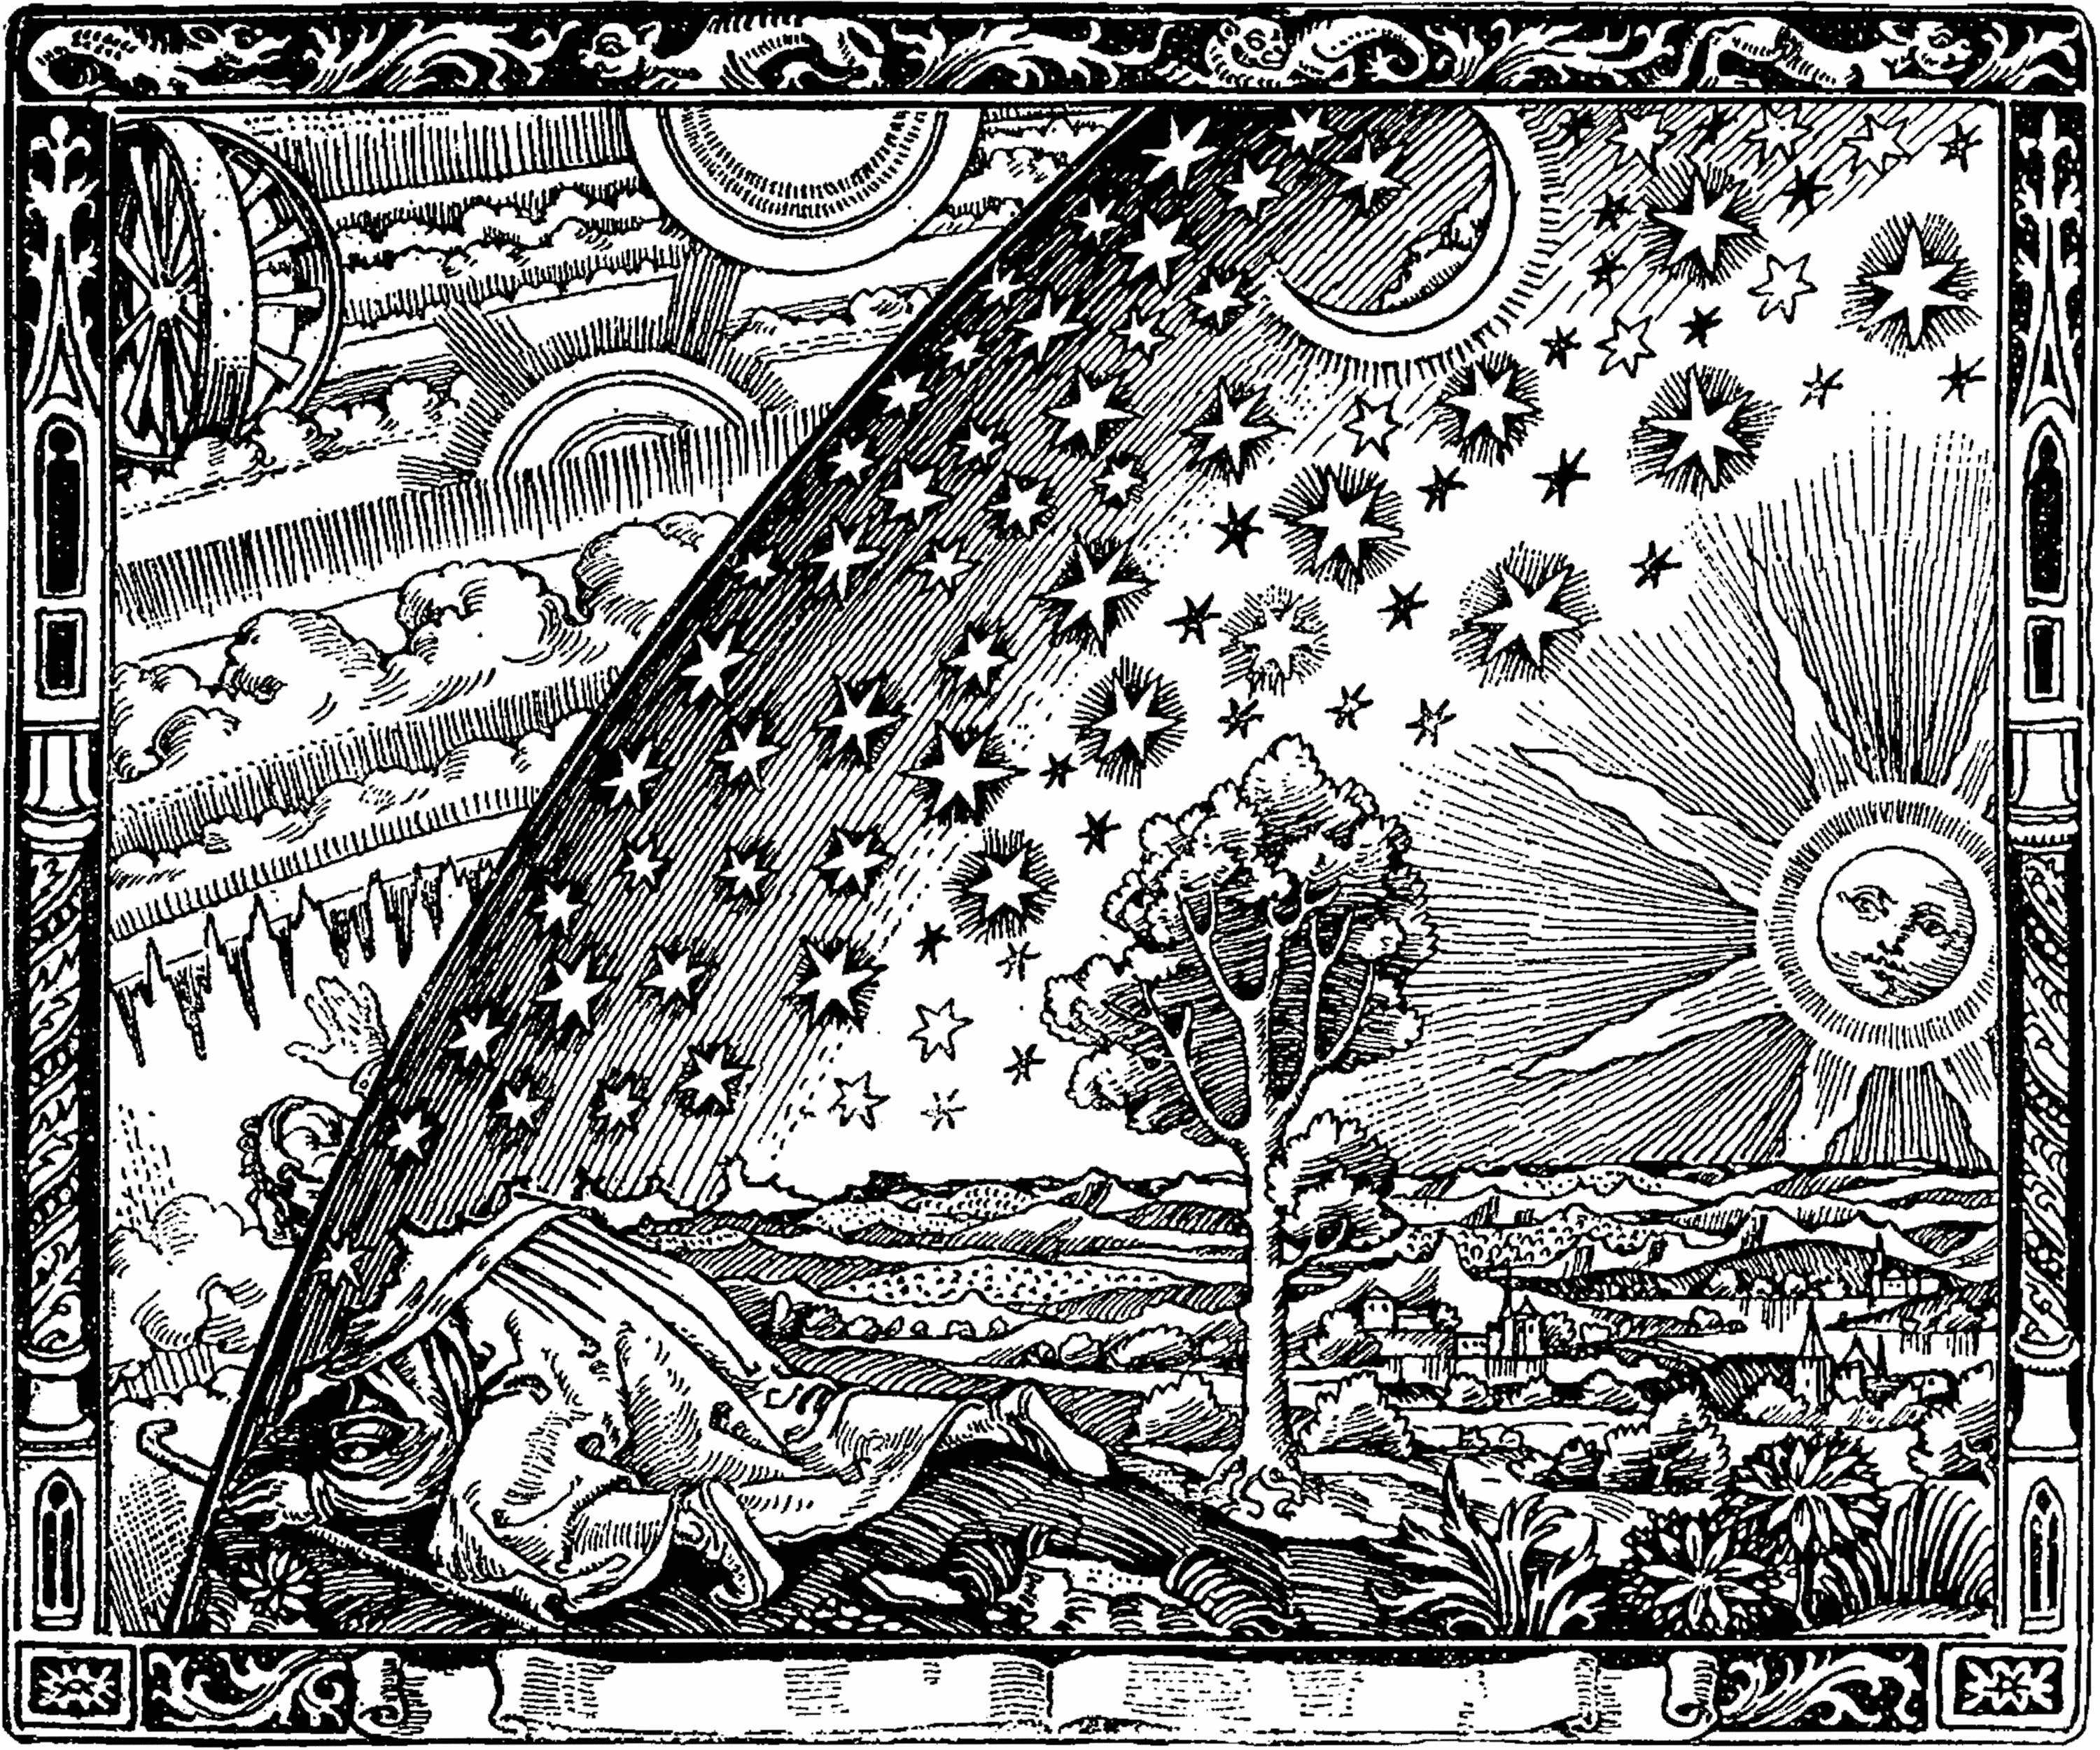
\includegraphics[width=\textwidth]{flammarion.jpg}
\end{figure}

\begin{center}
\textsc{Sint-Pieterscollege Leuven}
\end{center}

\vfill

%\clearpage
%\newpage
\tableofcontents
%\documentclass[12pt,numbers,noauthor,nooutcomes,wordchoicegiven]{xourse}
\documentclass{xourse}

\addPrintStyle{.}

\pdfOnly{
    \renewcommand{\xmcursusnaam}{{\textsc{Natuurkunde}}}
}

\logo{xmPictures/nomlogo.png}

\begin{document}
%	\setcounter{tocdepth}{2}
    \xmtitle{Inleiding}{}  
 


\part{Inleiding}

\activitychapter{../6dejaar/inleiding.tex}



\end{document}
%!TEX root = ../cursustekst_fys6.tex

\null\thispagestyle{empty}

\vfill

\begin{center}
\textsc{DEEL I}
\end{center}
\begin{center}
\textsc{\LARGE KINEMATICA}
\end{center}

\vfill

\begin{figure}[h]
\centering
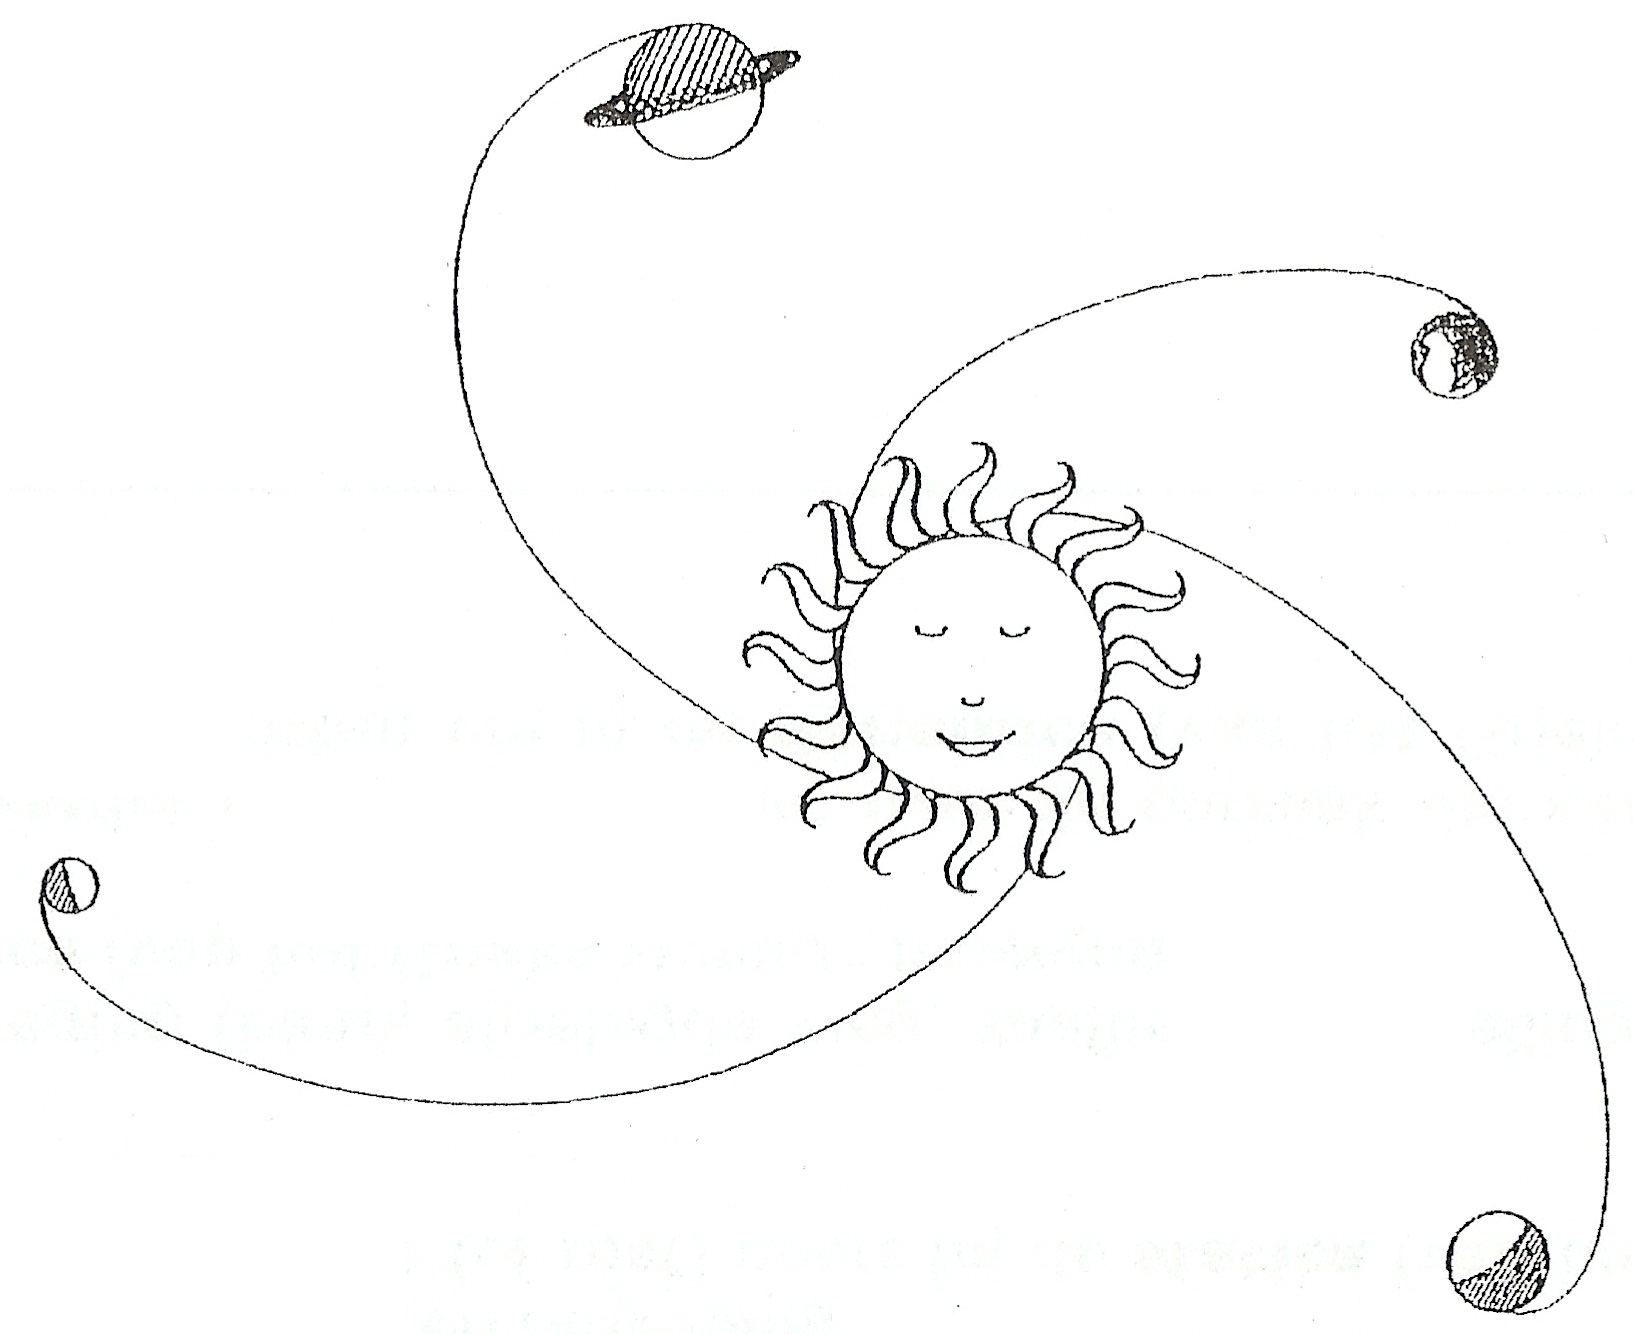
\includegraphics[width=0.7\textwidth]{zon_kinematica}
\end{figure}

\vfill

\clearpage
\newpage

% !TEX root = ../fys_cursus.tex



\chapter{Eendimensionale bewegingen}

Beweging beschrijven is niet zo simpel als het in eerste instantie lijkt. Zo is bijvoorbeeld de beweging van een wolk eerder complex. Wat reken je al dan niet tot de wolk? Ook de bewegingen van de afzonderlijke moleculen in kaart brengen is een onmogelijke opgave omdat het aantal moleculen eerder groot is. Om toch vooruitgang te kunnen boeken, beginnen we met voorwerpen die we als een punt kunnen voorstellen. We maken dan abstractie van de ruimtelijke vorm van het object dat we beschrijven en doen alsof we het kunnen reduceren tot \'e\'en enkele plaats in de ruimte. Zo zouden we het vliegen van een vlieg doorheen de kamer kunnen bekijken als een stipje. Het bewegen van de vleugels of de ori\"entatie van de kop van de vlieg laten we dan buiten beschouwing. Ook deze beschrijving kunnen we inperken; we gaan in eerste instantie enkel bewegingen beschrijven die voor te stellen zijn op een rechte lijn. Dit noemen we eendimensionale bewegingen. Als we de beschrijving hiervan eenmaal kennen, kunnen we later dit met behulp van vectoren gemakkelijk uitbreiden naar een beschrijving van bewegingen in twee- of drie dimensies.

Om het ons gemakkelijk te maken, zullen we in dit hoofdstuk enkel werken met de getalcomponenten van de vectoren. Dat gaat omdat we steeds in \'e\'en dimensie werken en de eenheidsvector dan steeds gelijk blijft. Als we $v_x$ kennen, vinden we direct de vectorcomponent volgens de $x$-as met $\vec{v}_x=v_x\cdot\vec{e}_x$. Bovendien kunnen we de index $x$ ook weglaten. We weten dat het steeds over de $x$-as gaat.

\section{Enkele begrippen}
\subsection{Positie en plaatsfunctie}

Het beschrijven van de beweging van een puntmassa kunnen we doen door de positie in de ruimte te geven in functie van de tijd. We kunnen m.a.w. een functie gebruiken die de plaats in functie van de tijd geeft. We noemen deze functie de \emph{plaatsfunctie} $x(t)$. $x$ staat voor de positie op een co\"ordinaatas\footnote{Een co\"ordinaatas is een as van een cartesiaans assenstelsel, met een oorsprong en een ori\"entatie.} en $t$ is de variabele die symbool staat voor de tijd\footnote{In de fysica gebruiken we de wiskunde als `taal' om de wetmatigheden van de natuur in uit te drukken. Wiskundige variabelen en objecten zoals functies krijgen nu een fysische betekenis. $x(t)$ is dus niets anders dan een functie $f(x)$ of $y(x)$ zoals je die in wiskunde kent. Alleen nemen wij nu niet voor de onafhankelijke variabele het symbool $x$ maar het symbool $t$ omdat deze symbool moet staan voor de tijd. En voor het symbool $f$ gebruiken wij nu het symbool $x$ omdat de beeldwaarden van de functie nu als betekenis een positie op een co\"ordinaatas hebben.}. Een notatie voor een bepaalde posities \footnote{Natuurlijk kan de index 1 ook vervangen worden door andere indices. Voorbeelden zijn $x_0=x(t_0)$ en $x_2=x(t_2)$.} op de co\"ordinaatas op een bepaald tijdstip $t_1$, is:
\begin{eqnarray*}
x_1=x(t_1)
\end{eqnarray*}
Zo zie je in figuur (\ref{grafplaatsfunctie}) een auto op verschillende tijdstippen $t_0,t_1, t_2,\ldots$ weer\-ge\-ge\-ven op verschillende posities. Je ziet ook een grafiek van de bijbehorende plaatsfunctie.

\begin{figure}[h]
\hfill
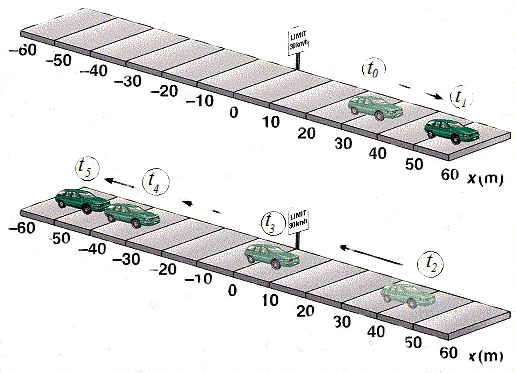
\includegraphics[width=0.45\textwidth]{Serway2p1(1)}
\hfill
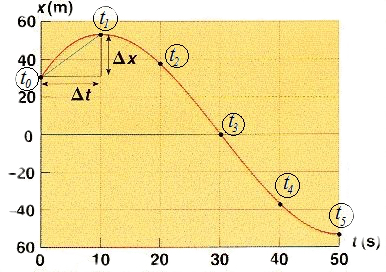
\includegraphics[width=0.45\textwidth]{Serway2p1(2)}
\hfill
\caption{Verschillende posities en de grafiek van de plaatsfunctie}
\label{grafplaatsfunctie}
\end{figure}

Het verschil tussen twee co\"ordinaten noemen we de \emph{verplaatsing}:
\[
\Delta x = x_2-x_1
\]
Zo is de verplaatsing van de auto in de figuur tussen de tijdstippen $t_0$ en $t_1$ gelijk aan $\Delta x = x_1-x_0=50\rm\,m-30\rm\,m=20\rm\,m$ en is de verplaatsing tussen de tijdstippen $t_2$ en $t_4$ gelijk aan $\Delta x=x_4-x_2=-40\rm\,m-40\rm\,m=-80\rm\,m$. Deze laatste verplaatsing is negatief, wat aangeeft dat de auto netto naar achteren is bewogen -- tegengesteld aan de zin van de gekozen as.
\newline
Let op, de verplaatsing hoeft niet noodzakelijk gelijk te zijn aan de \emph{afgelegde weg} tussen de twee bijbehorende tijdstippen. Als je op caf\'e na naar het toilet te zijn geweest terug op je oorspronkelijke plaats op het terras gaat zitten, is je (netto) verplaatsing nul maar heb je wel degelijk afstand afgelegd.

\subsection{Gemiddelde snelheid}

De gemiddelde snelheid $\overline{v}$ \footnote{Als symbool voor de gemiddelde snelheid wordt ook $<v>$ gebruikt.} van een voorwerp tussen twee tijdstippen defini\"eren we als de verplaatsing over het benodigde tijdsinterval.
\begin{eqnarray*}
\overline{v}=\frac{\Delta x}{\Delta t}=\frac{x_2-x_1}{t_2-t_1}
\end{eqnarray*}
De eenheid van snelheid is bijgevolg meter per seconde $[v]=\rm\,m/s$. Als voorbeeld is de gemiddelde snelheid van de auto in figuur (\ref{grafplaatsfunctie}) tussen de tijdstippen $t_1$ en $t_2$ gelijk aan $\overline{v}=\frac{x_2-x_1}{t_2-t_1}=\frac{40\rm\,m-50\rm\,m}{20\rm\,s-10\rm\,s}=-1\rm\,m/s$. Dat de snelheid negatief is, betekent natuurlijk dat de auto achteruit rijdt.

\subsection{Gemiddelde versnelling}

Zoals we bij snelheid kijken hoe de positie verandert gedurende de tijd, kunnen we ons ook afvragen hoe de snelheid verandert gedurende de tijd. Dit idee ken je al, we noemen het versnellen of vertragen.

De gemiddelde versnelling tussen twee tijdstippen defini\"eren we als de verandering van de snelheid in het bijbehorende tijdsinterval.
\begin{eqnarray*}
\overline{a}=\frac{\Delta v}{\Delta t}=\frac{v_2-v_1}{t_2-t_1}
\end{eqnarray*}
De eenheid van versnelling is bijgevolg meter per seconde, per seconde -- wat meter per seconde in het kwadraat geeft $[a]=\rm\,m/s^2$.

\subsection{Ogenblikkelijke snelheid}

Zoals we een voorwerp op een bepaald tijdstip een positie toekennen, willen we het voorwerp ook een snelheid op een bepaald tijdstip toekennen. Dat is echter moeilijker dan je denkt. Want wanneer we het over snelheid hebben, moeten we spreken over het aantal meter dat in een bepaald tijds\-in\-ter\-val wordt afgelegd. Het probleem is dat op \'e\'en bepaald moment, \'e\'en ogenblik, er helemaal geen tijdsverloop is en we bijgevolg ook geen verplaatsing kunnen hebben\ldots! Er is immers geen tijd verstreken om afstand te kunnen afleggen.`Ja, maar', ga je zeggen, `de snelheidsmeter van mijn fiets zegt toch hoe hard ik ga?!' Dat \emph{lijkt} inderdaad een ogenblikkelijke snelheid te zijn maar in werkelijkheid is dat steeds de gem\'iddelde snelheid over het \mbox{tijds}\-in\-ter\-val dat het sensortje op je wiel nodig heeft om \'e\'en omwenteling te maken. Je snelheidsmeter berekent dus de gemiddelde snelheid door je wielomtrek\footnote{Die je hebt moeten ingeven\ldots} te delen door de tijd van \'e\'en omwenteling. Als jij plots remt gaat je snelheid afnemen maar je metertje gaat dit niet ogenblikkelijk kunnen aangeven. Het moet wachten totdat het sensortje weer rond is geweest om de tijd te kennen en zo de snelheidsverandering te kunnen registreren.
\begin{figure}[h]
\centering
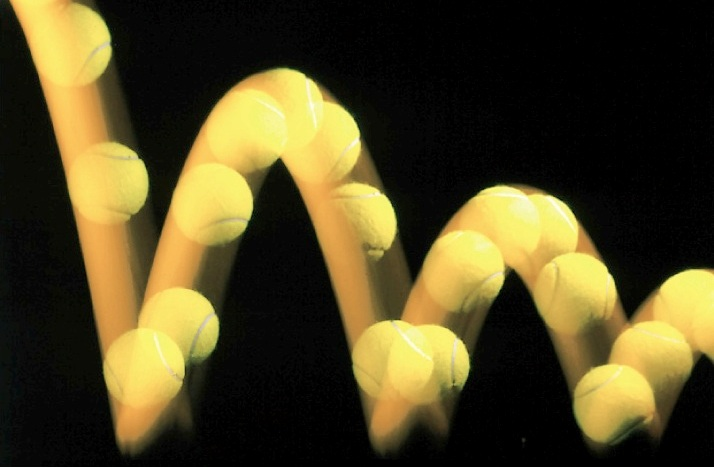
\includegraphics[width=0.8\textwidth]{stuiterendetennisbal}
\caption{Stuiterende tennisbal}\label{stuiterendetennisbal}
\end{figure}
Hoe lossen we dit probleem nu op? Als we naar de stroboscopische foto (\ref{stuiterendetennisbal}) van de stuiterende tennisbal kij\-ken, zien we dat de bal bovenaan trager beweegt dan wanneer hij de grond nadert. Bovenaan liggen de beelden immers dichter bij elkaar zodat de tennisbal minder afstand aflegt in de tijdsspanne tussen twee opeenvolgende opnames. 
De kwantitatieve\footnote{Kwantitatief wil zeggen dat het over een hoeveelheid of een grootte gaat.} informatie die we op deze manier uit de beelden kunnen destilleren, levert ons echter opnieuw gemiddelde snelheid en niet zomaar de ogenblikkelijke snelheid. De tennisbal verandert immers nog van snelheid tussen twee opeenvolgende opnames. Door nu echter de frequentie\footnote{Frequentie is een grootheid die aangeeft hoeveel cyclussen er per seconde worden doorlopen. Hier gaat het dus over het aantal beelden dat per seconde wordt gemaakt. De eenheid van frequentie is $\rm\,s^{-1}$ oftewel Hz (de Hertz).} waarmee de foto's worden genomen op te drijven, krijgen we een accurater beeld van de snelheid die de tennisbal op een gegeven moment heeft. De tijdsintervallen zijn nu immers korter zodat de bal minder van snelheid kan veranderen gedurende de intervallen en zodoende de gemiddelde snelheid een indicatie wordt van de ogenblikkelijke snelheid. De ogenblikkelijke snelheid wordt dus beter en beter benaderd door het tijdsinterval kleiner en kleiner en kleiner en kleiner\ldots te nemen. Echter, hoe kort het tijdsinterval ook is, de snelheid zal veranderen gedurende dat hele kleine tijdsinterval. Daarom, je raadde het misschien al lang, defini\"eren we de ogenblikkelijke snelheid als de \emph{limiet} van de gemiddelde snelheid over een tijdsinterval waarbij we dat interval naar nul laten gaan. Of m.a.w. wordt de ogenblikkelijke snelheid gedefinieerd \footnote{Dat betekent dus dat als iemand je vraagt wat snelheid is, je moet antwoorden dat het de afgeleide\ldots} als de afgeleide\footnote{De afgeleide is in deze context van het zoeken naar snelheid door Isaak Newton (1643-1727) en Gottfried Wilhelm von Leibniz (1646-1716) onafhankelijk van elkaar ontwikkeld.} van de plaatsfunctie:
\begin{eqnarray*}
v=\lim_{\Delta t\to 0}\frac{\Delta x}{\Delta t}=\lim_{t\to t_0}\frac{x(t)-x(t_0)}{t-t_0}=\frac{dx}{dt}
\end{eqnarray*}
We noteren dit ook zoals in de wiskunde met een accent $v(t)=x'(t)$ of $v=x'$. $v(t)$ is opnieuw een functie die op elk moment de snelheid geeft. 

Grafisch weet je dat je de afgeleide kan terugvinden als de richtingsco\"effici\"ent van de raaklijn. In een $x-t$ grafiek (de grafiek van de functie $x(t)$, $x$ in functie van $t$) vind je dus de snelheid als de richtingsco\"effici\"ent van een raaklijn in het beschouwde punt. 

Opmerking: Het woord 'ogenblikkelijk' mag je ook weglaten. Wanneer we het over snelheid hebben, bedoelen we vanaf nu steeds ogenblikkelijke snelheid.

\subsection{Ogenblikkelijke versnelling}

Voor een ogenblikkelijke verandering van de snelheid maken we eenzelfde redenering als voor de ogenblikkelijke verandering van de positie. De ogenblikkelijke versnelling wordt dus m.a.w. gewoonweg de afgeleide van de snelheid:
\begin{eqnarray*}
a=\lim_{t\to t_0}\frac{v(t)-v(t_0)}{t-t_0}&=&\frac{dv}{dt}=\frac{d^2x}{dt^2}
\end{eqnarray*}
Ook hier hanteren we eveneens een notatie m.b.v. accenten $a(t)=v'(t)=x''(t)$ en bedoelen we met versnelling, ogenblikkelijke versnelling.

\section{ERB}

De \emph{eenparig rechtlijnige beweging} (afgekort ERB) is een specifieke beweging. De snelheid van de beweging is eenparig of gelijkmatig verdeeld wat betekent dat de snelheid steeds gelijk blijft. M.a.w. is de snelheid constant of is de versnelling nul. Omdat de snelheid niet verandert is de ogenblikkelijke snelheid gelijk aan de gemiddelde snelheid en kunnen we gemakkelijk een functie vinden voor de positie in functie van de tijd:
\begin{eqnarray*}
v=\frac{\Delta x}{\Delta t}&\Leftrightarrow&\Delta x=v\Delta t\\
&\Leftrightarrow&x-x_0=v(t-t_0)\\
&\Leftrightarrow&x=x_0+v(t-t_0)
\end{eqnarray*}
Samengevat:

\kader{
%\vspace{3mm}
De plaatsfunctie $x(t)$ van een ERB met snelheid $v$ is gegeven door:
\begin{eqnarray}\label{x(t)ERB}
x(t)&=&x_0+v(t-t_0)
\end{eqnarray}
waarbij $x_0=x(t_0)$ de co\"ordinaat op het tijdstip $t_0$ is. Indien $t_0=0$ dan vereenvoudigt de plaatsfunctie (\ref{x(t)ERB}) tot
\begin{eqnarray}\label{x(t)ERB0}
x(t)&=&x_0+vt
\end{eqnarray}
%\vspace{0mm}
}

Aangezien de snelheid van een ERB constant is, is de beginsnelheid $v_0=v(t_0)$ gelijk aan de snelheid $v$, $v_0=v$. De snelheidsfunctie is natuurlijk $v(t)=v$ en de versnellingsfunctie is $a(t)=0$.
\begin{figure}[h]
\centering
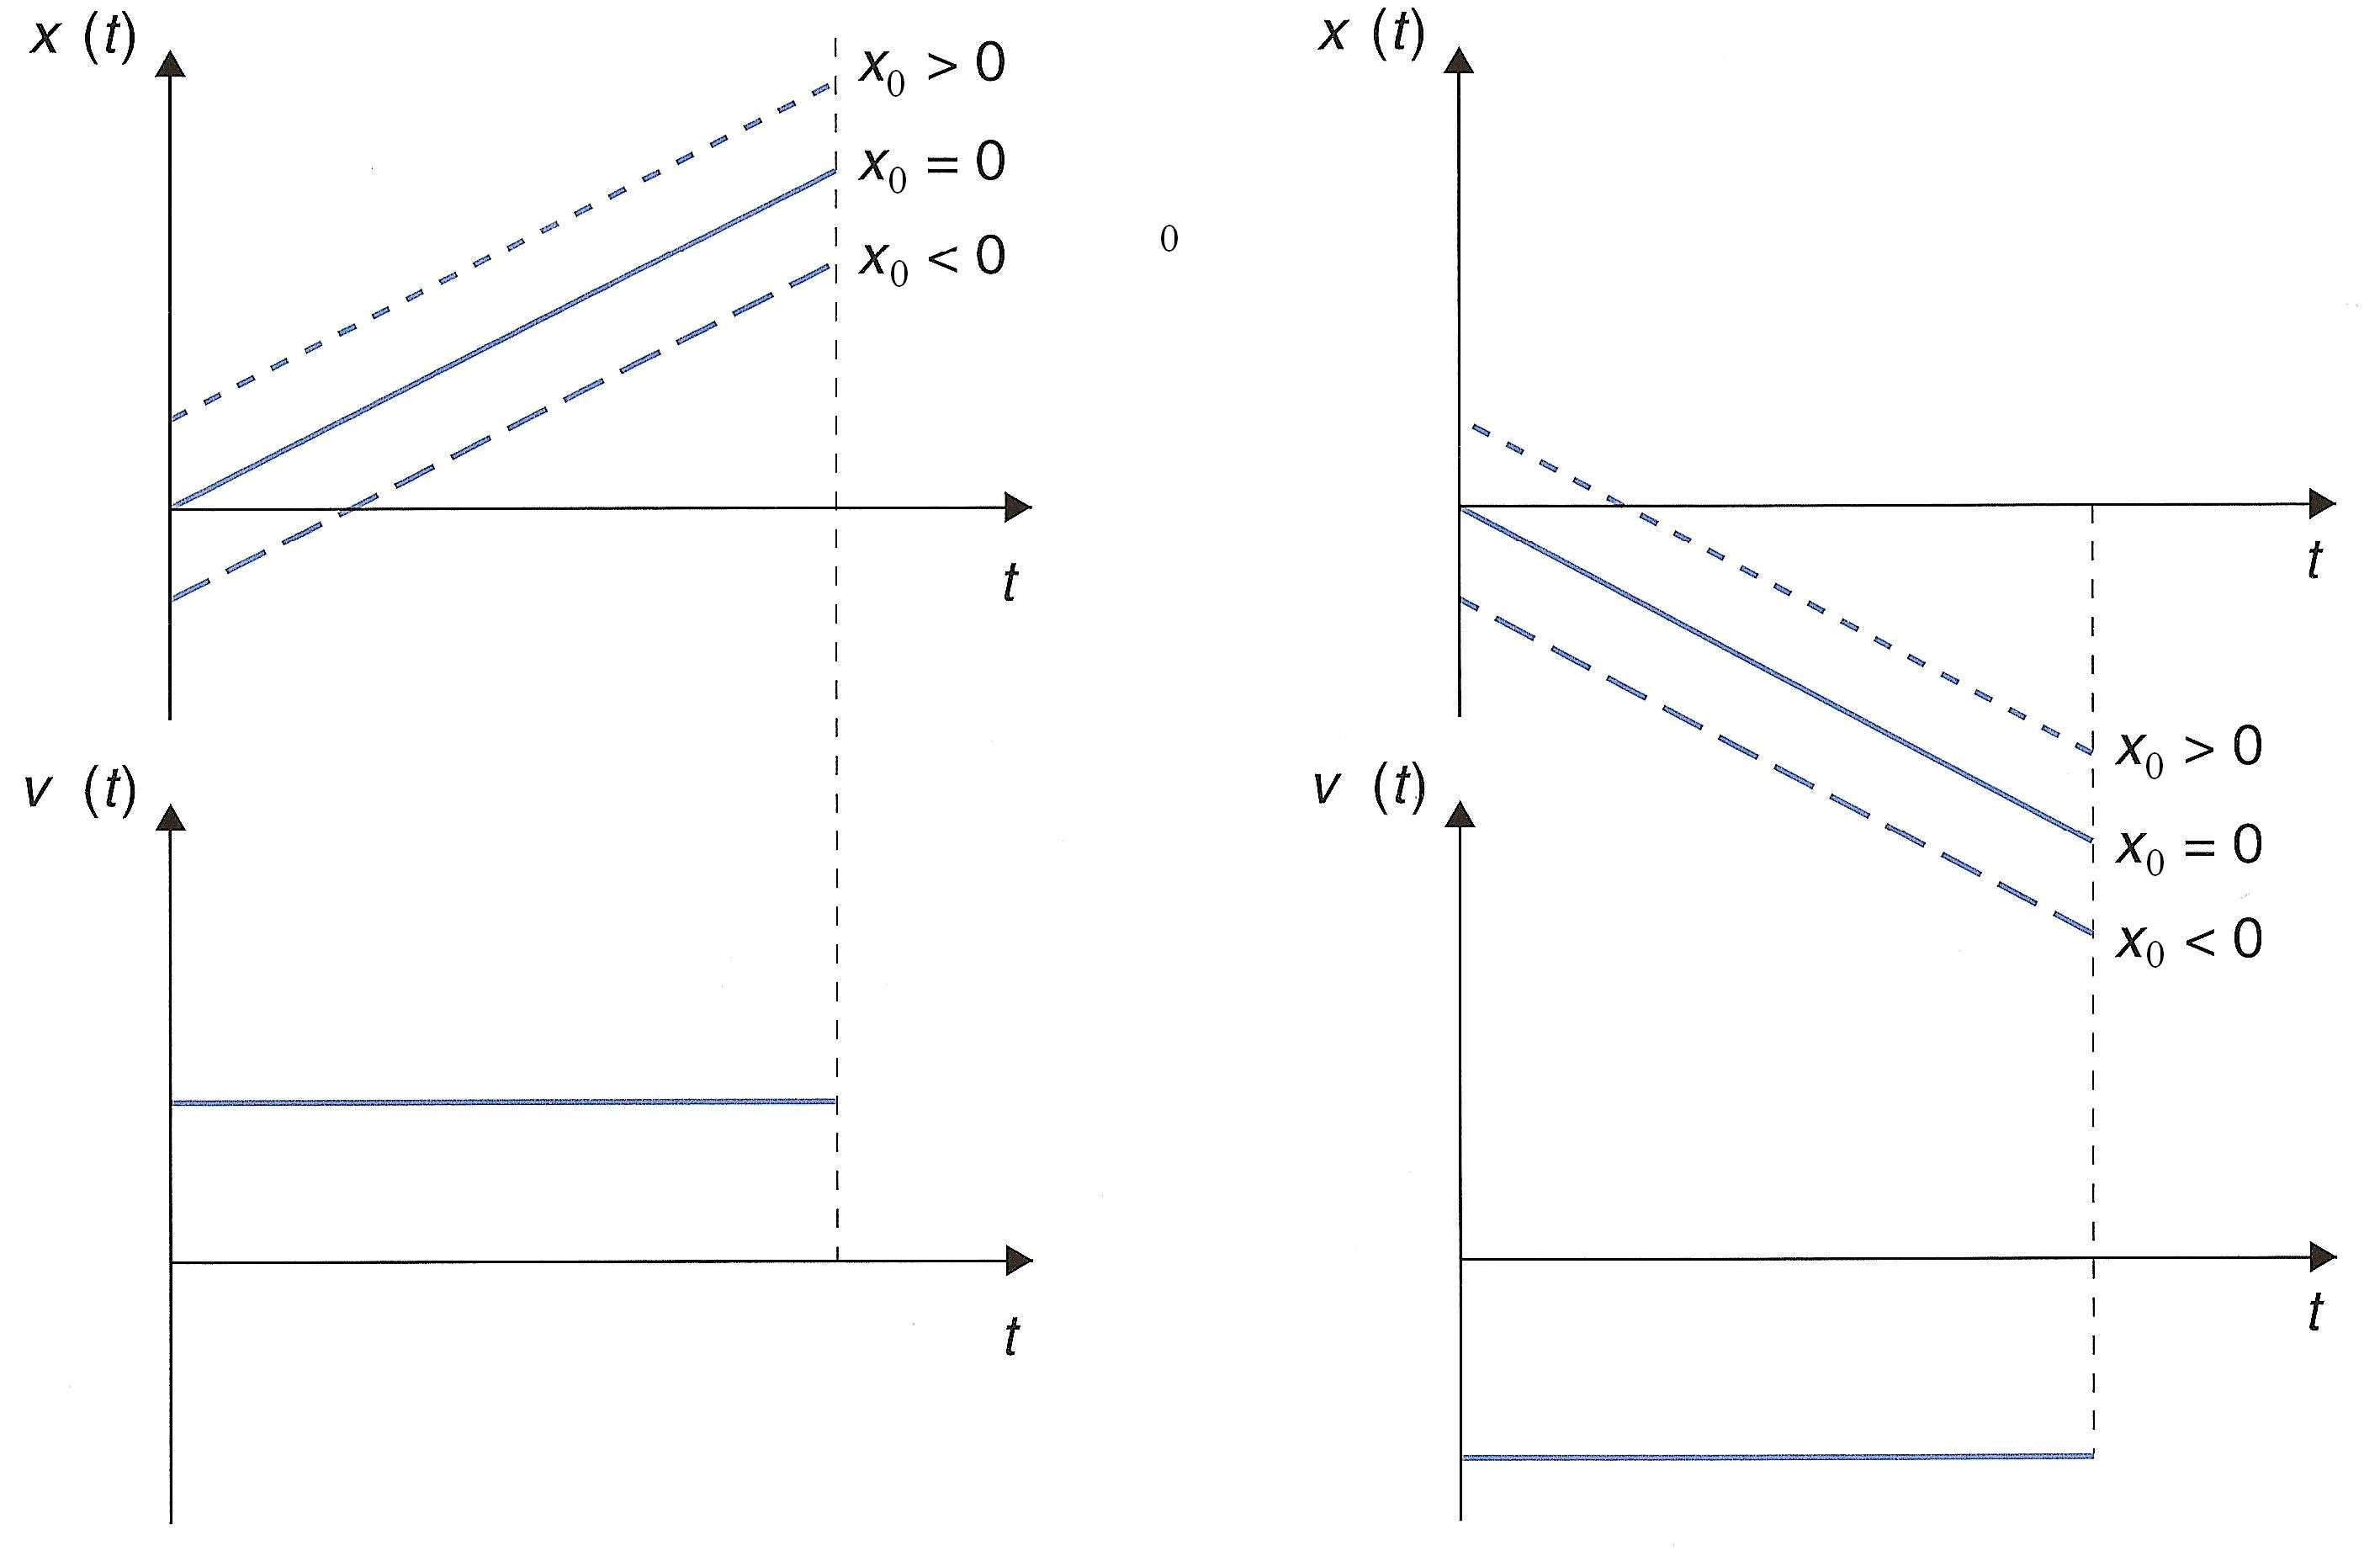
\includegraphics[width=.7\textwidth]{ERB_grafieken}
\caption{Grafieken van een ERB}
\end{figure}









\cleardoublepage
\setcounter{page}{1}
\setcounter{footnote}{0}
\setcounter{figure}{0}
\setcounter{equation}{0}
% 2021-2022: Aangepaste en verbeterde versie om als afzonderlijke bij lage aan de lln te kunnen geven.

\section{EVRB}

\section*{C Eenparig veranderlijke rechtlijnige beweging}

Een beweging waarvan de versnelling constant is, noemen we een \textit{eenparig veranderlijke rechtlijnige be\-we\-ging}, afgekort EVRB. Eenparig betekent gelijkmatig; de snelheidsverandering is steeds gelijk. In symbolen geldt dus dat $a(t)=a$ waarbij het maatgetal van $a$ een re\"eel getal is. We werken voor dit model de plaatsfunctie en de snelheidsfunctie uit. M.a.w. willen we het verloop van de plaats en de snelheid in functie van de tijd kennen. 

Aangezien de versnelling constant is en de versnelling de afgeleide van de snelheid, moet de snelheid in functie van de tijd een lineaire functie (in de tijd) zijn.\footnote{Strikt genomen zien we hier iets over het hoofd. A priori zou het immers kunnen dat er nog andere functies dan lineaire functies zijn waarvoor de afgeleide een constante functie is. Dat is echter niet het geval. Het bewijs hiervan zie je later dit jaar in het vak wiskunde. Je bewijst dat alle mogelijke functies die in aanmerking komen slechts op een constante na aan elkaar gelijk zijn.} Nu dat we het snelheidsverloop kennen, kunnen we het verloop van de plaats afleiden. Aangezien de snelheid een lineaire functie is en de snelheid de afgeleide van de positie is, moet de positie een kwadratische functie (in de tijd) zijn. De afgeleide van een kwadratische functie is immers een lineaire functie.\footnote{Hier geldt een gelijkaardige opmerking als die in de vorige voetnoot.}

Dat de positie in functie van de tijd een tweedegraadsveeltermfunctie is, geeft in symbolen:\footnote{we gebruiken de constanten $p$, $q$ en $r$ i.p.v. $a$, $b$ en $c$ om verwarring met de betekenis van $a$ te voorkomen.}
\begin{eqnarray}
x(t)=pt^2+qt+r\label{pqr}
\end{eqnarray}
Nu willen we de constanten $p$, $q$ en $r$ fysisch kunnen duiden en eventueel andere symbolen geven, zodat hun betekenis sneller af te lezen is. Dat doen we door te eisen dat de afgeleide met de snelheid overeenkomt en de tweede afgeleide met de versnelling. Ook gebruiken we de beginvoorwaarden. Dus:
\begin{align}
v(t)&=\frac{dx}{dt}=2pt+q\label{2pq}\\
a(t)&=\frac{d^2x}{dt^2}=2p\nonumber
\end{align}
Omdat de versnelling constant is, halen we uit de laatste regel dat $a(t)=a=2p\Leftrightarrow p=\frac{a}{2}$. Als we met $v_0$ de snelheid op tijdstip $t=0$ voorstellen ($v_0=v(0)$) en $t=0$ invullen in (\ref{2pq}), dan vinden we dat $q=v_0$. De constante $q$ stelt dus de beginsnelheid voor. Als we vervolgens met $x_0$ de positie op tijdstip $t=0$ voorstellen en $t=0$ invullen in (\ref{pqr}), dan vinden we dat $r=x_0$. De constante $r$ stelt dus de beginpositie voor.

Samengevat levert dat:

\kader{
%\phantom{}
\vspace{1ex}
De plaatsfunctie $x(t)$ en de snelheidsfunctie $v(t)$ van een EVRB met versnelling $a$ worden gegeven door:
\begin{eqnarray}
x(t)&=&x_0+v_0t+\frac{1}{2}at^2\label{x(t)0}\\
v(t)&=&v_0+at\label{v(t)0}
\end{eqnarray}
Hierin is $x_0$ de \textit{beginpositie} en $v_0$ de \textit{beginsnelheid}. Ze worden bepaald door de \textit{beginvoorwaarden} of \textit{randvoorwaarden}.
\vspace{1ex}
%\phantom{.}
}

Indien we de beschrijving van de beweging niet op $t=0$ willen laten starten maar op een gegeven tijdstip $t_0$, dan moeten we in de beschrijving $t$ vervangen door $\Delta t= t-t_0$, de verstreken tijd vanaf het begintijdstip $t_0$. De functies (\ref{x(t)0}) en (\ref{v(t)0}) worden dan een klein beetje ingewikkelder:
\begin{eqnarray}
x(t)&=&x_0+v_0(t-t_0)+\frac{1}{2}a(t-t_0)^2\label{x(t)}\\
v(t)&=&v_0+a(t-t_0)\label{v(t)}
\end{eqnarray}

Met de functies (\ref{x(t)}) en (\ref{v(t)}) kunnen we de volgende formule voor de gemiddelde snelheid van een EVRB aantonen:%\footnote{Het formuletje is handig te gebruiken in veel vraagstukken door gebruik te maken van $\Delta x=\overline{v}\Delta t$.} 
\footnote{De afleiding van de gemiddelde snelheid is als volgt:
\begin{eqnarray*}
\overline{v}=\frac{\Delta x}{\Delta t}=\frac{x-x_0}{t-t_0}=\frac{v_0(t-t_0)+\frac{1}{2}a(t-t_0)^2}{(t-t_0)}=\frac{2v_0+a(t-t_0)}{2}=\frac{v_0+v}{2}.
\end{eqnarray*}}
\begin{eqnarray*}
  \overline{v}=\frac{v_0+v}{2}
\end{eqnarray*}
Blijkbaar houdt het eenparig toenemen van de snelheid in dat we het rekenkundig gemiddelde kunnen gebruiken voor de gemiddelde snelheid.

\newpage

\begin{figure}[h]
\centering
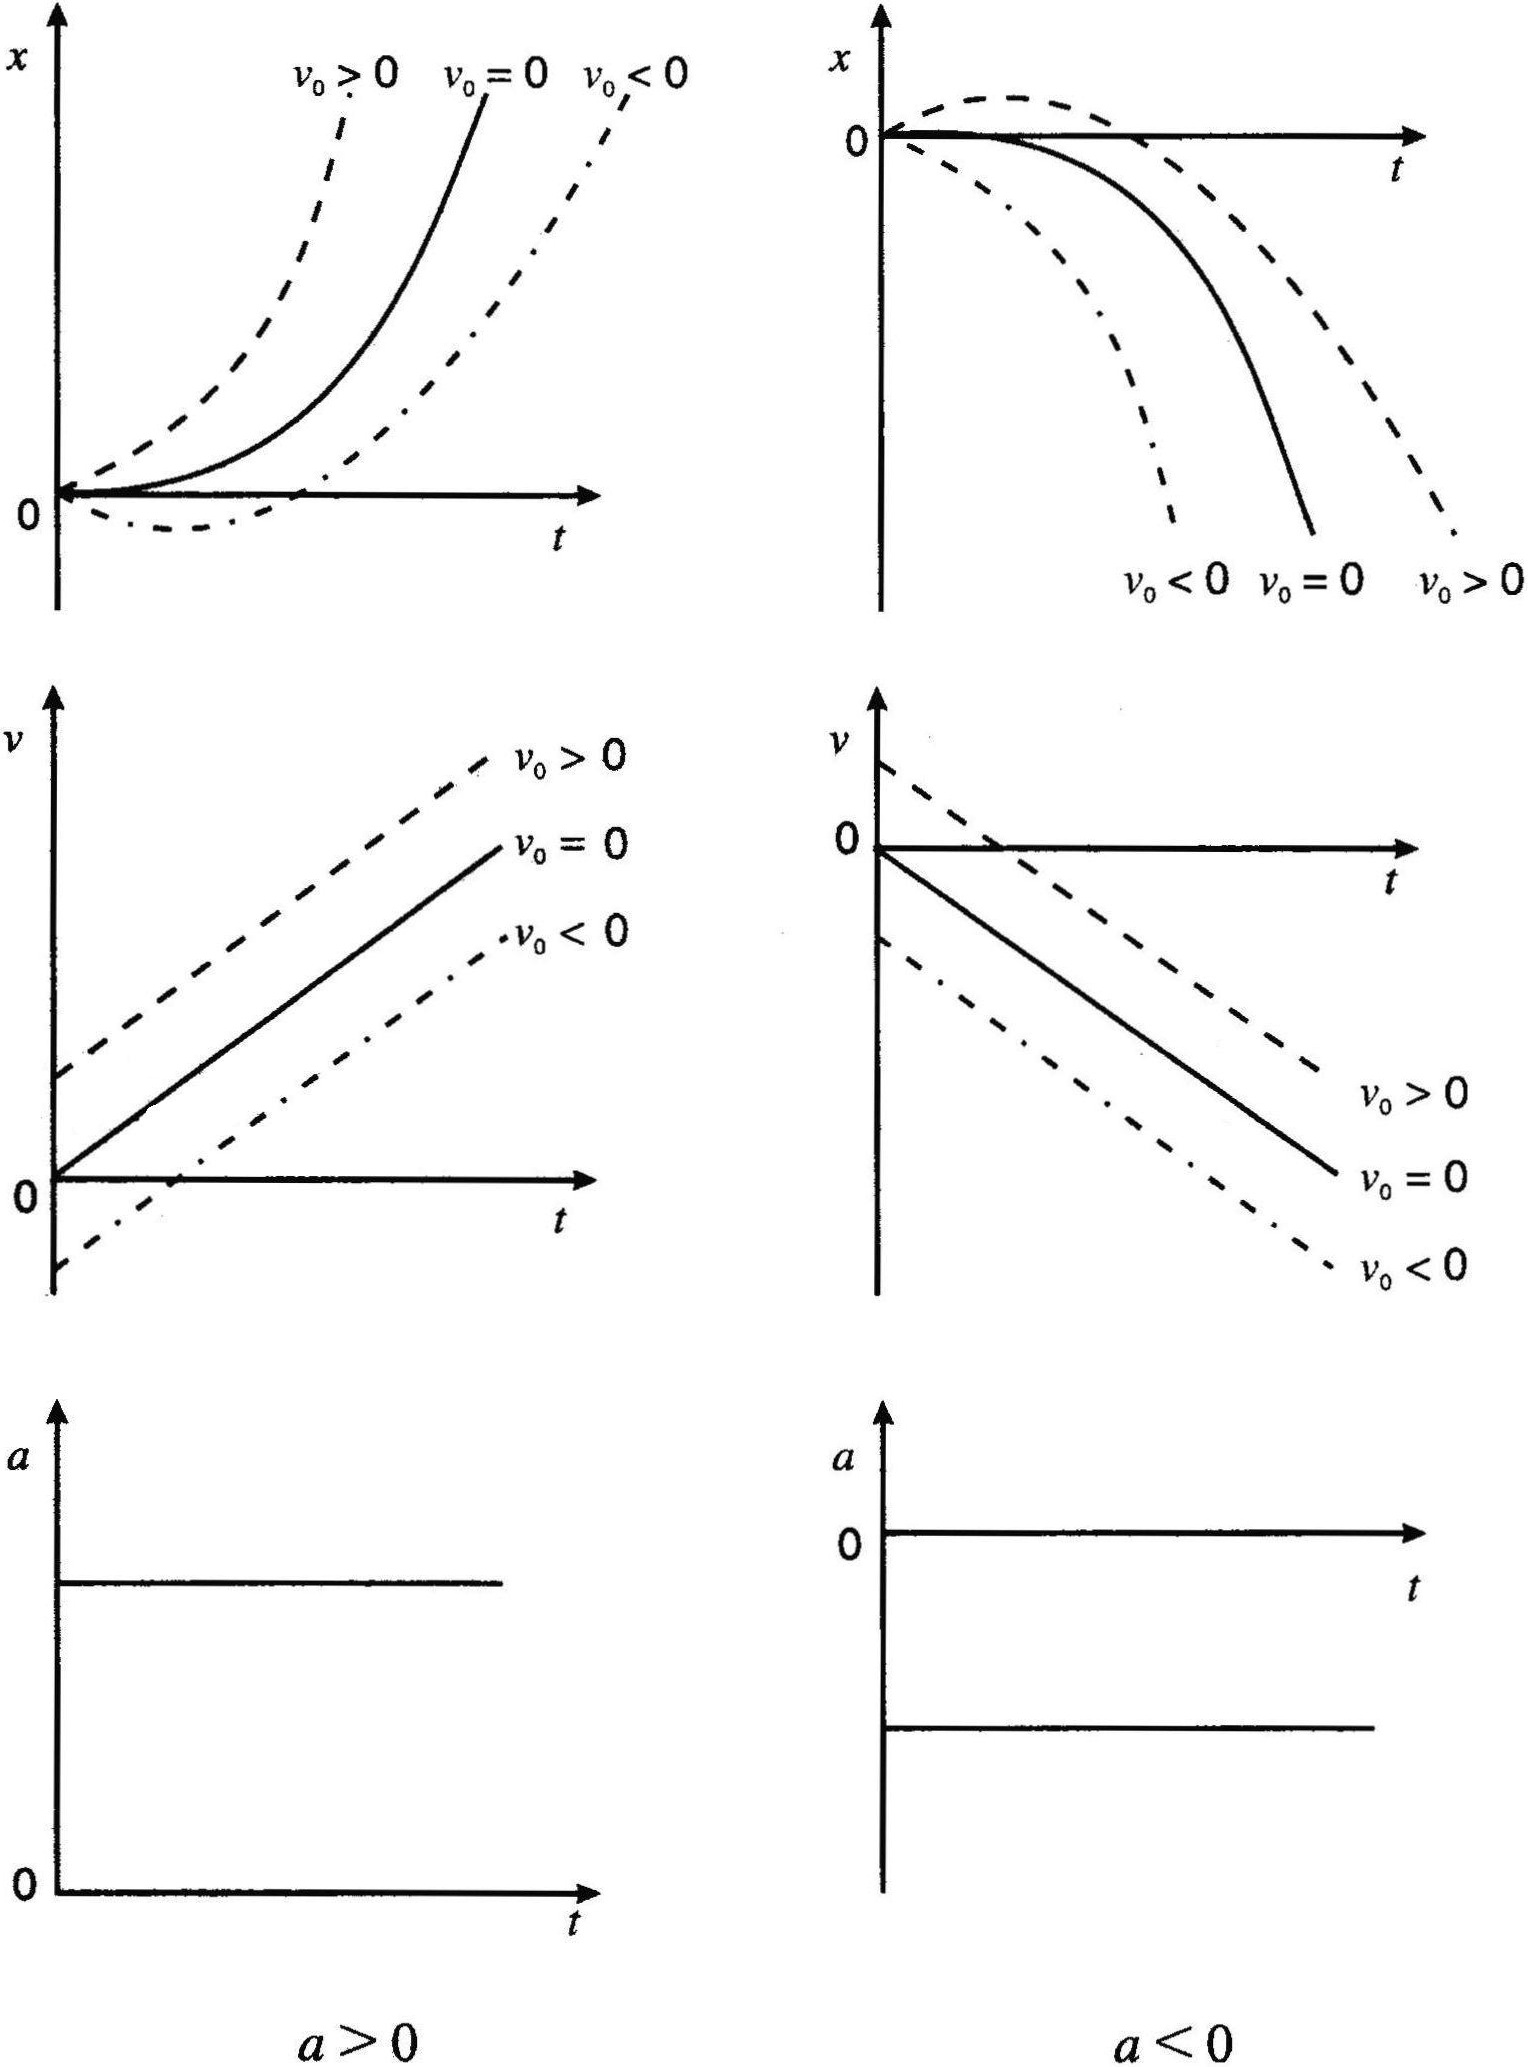
\includegraphics[width=\textwidth]{EVRB_grafieken}
%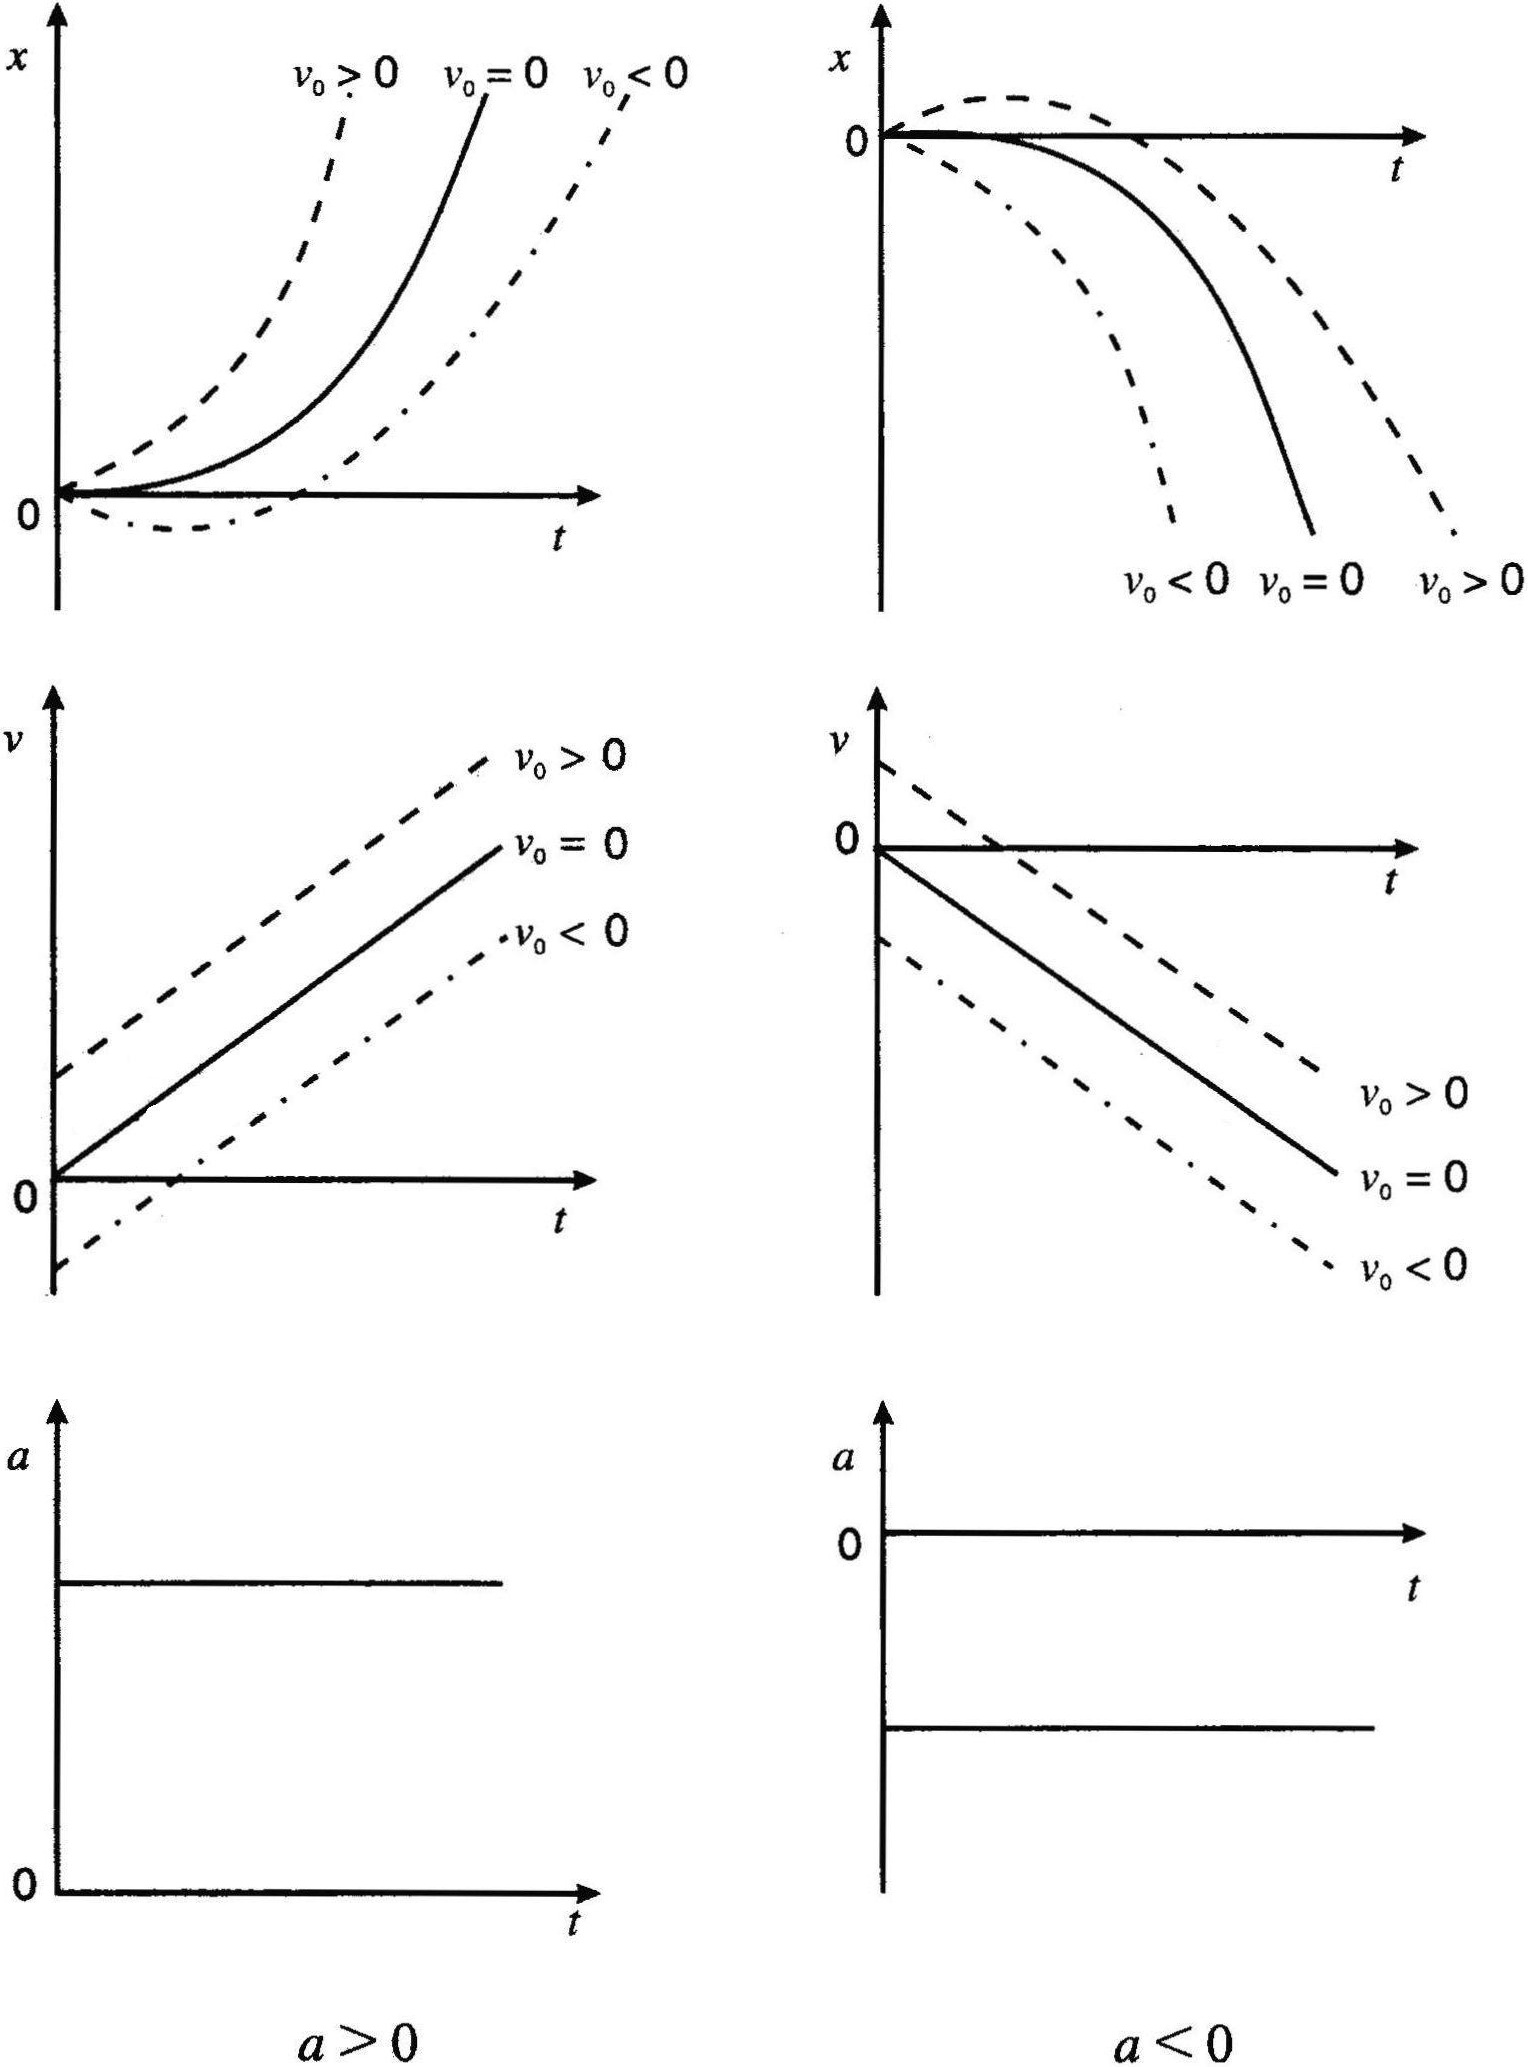
\includegraphics[height=\textheight]{EVRB_grafieken}
\caption{Grafieken van een EVRB}
\end{figure}

\clearpage
\newpage
\thispagestyle{empty}

\section*{Voorbeeldoefening}

\begin{enumerate}

\item[\textbf{Opgave}]\textsf{Een auto die $\SI{60}{km/h}$ rijdt, raakt een boom; de voorkant van de auto wordt in elkaar gedrukt en de bestuurder komt na $\SI{70}{cm}$ tot stilstand. Welke gemiddelde vertraging onderging de bestuurder tijdens de botsing? Druk je antwoord uit in $g$, waarbij $g=\SI{9,81}{m/s^2}$.
\item[\textit{Gegeven}]$v_0=\SI{16,7}{m/s}$\newline$x=\SI{0,70}{m}$
\item[\textit{Gevraagd}]$a$
\item[\textit{Oplossing}] Om de (constante) vertraging te vinden, hebben we de snelheidsverandering en de benodigde tijd nodig. De verandering in snelheid kennen we; de eindsnelheid van de auto moet nul worden maar de duur is niet onmiddellijk gegeven. Omdat de eindsnelheid nul is, kunnen we wel uit de snelheidsvergelijking van een eenparig veranderlijke beweging een \emph{uitdrukking} vinden voor die tijd die we vervolgens kunnen substitueren in de plaatsvergelijking. De enige onbekende is dan de gezochte versnelling.\footnote{M.b.v. de formule $\overline{v}=\frac{v_0+v}{2}$ voor de gemiddelde snelheid en de definitie voor de gemiddelde snelheid $\overline{v}=\frac{\Delta x}{\Delta t}$ is het antwoord sneller te vinden. Ga maar na \ldots}
\newline
\newline
Uit $v(t)=0$ of $0=v_0+at$ halen we een uitdrukking voor de tijd die nodig is om tot stilstand te komen:
\begin{align*}
t&=-\frac{v_0}{a}
\end{align*}
Substitutie van deze tijd in de plaatsfunctie levert:
\begin{align*}
x&=v_0t+\frac{1}{2}at^2\\
&=v_0\left(-\frac{v_0}{a}\right)+\frac{1}{2}a\left(-\frac{v_0}{a}\right)^2\\
%&=&-\frac{v_0^2}{a}+\frac{v_0^2}{2a}\\
&=-\frac{v_0^2}{2a}\\
\end{align*}
De versnelling is dan gelijk aan:
\begin{align*}
a&=-\frac{v_0^2}{2x}
\end{align*}
Invullen van de gegevens levert $a=\SI{-198}{m/s^2}$, wat gelijk is aan $20g$.
}
\end{enumerate}

\newpage










\section{Verticale worp}

Onze perceptie van vallende voorwerpen is dat zwaardere lichamen sneller vallen dan lichtere. Een veertje en een hamer komen in de regel niet tegelij\-ker\-tijd op de grond terecht. Wanneer we echter voorwerpen in vacu\"um\footnote{In vacu\"um ondervinden voorwerpen geen luchtweerstand.} laten vallen, blijkt de massa geen rol te spelen bij de constante versnelling die de voorwerpen krijgen -- alle voorwerpen vallen met dezelfde versnelling. De verklaring hiervoor hoort thuis in de dynamica. In de kinematica houden we ons enkel bezig met de beschrijving van de beweging. Aangezien de valversnelling constant is, hebben we simpelweg met een EVRB te maken.
\begin{figure}[h]
\centering
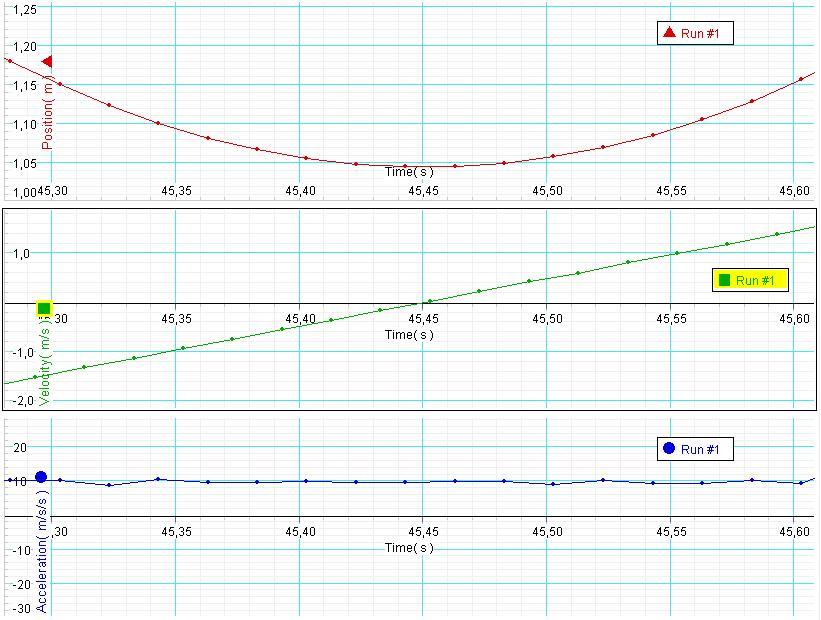
\includegraphics[width=0.85\textwidth]{valbeweging_pasco2}
\caption{Experimenteel bekomen grafieken van een verticale worp waarbij de as naar beneden is geori\"enteerd.}
\end{figure}
Strikt genomen verschilt de valversnelling van plaats tot plaats op de aarde, maar voor het gemak nemen wij in vraagstukken de waarde
\[g=9,81\rm\,m/s^2.\]
Omdat de verticale worp een EVRB is, kunnen we de formules (\ref{x(t)0}) en (\ref{v(t)0}) gebruiken om een valbeweging te beschrijven. Voor de versnelling $a$ nemen we dan $a=g$ of $a=-g$ al naargelang de ori\"entatie van de co\"ordinaatas.

\clearpage
\newpage


\begin{enumerate}
\item[\textbf{Opgave}]\textsf{Van de boord van een schip valt een loden bol in het water. De \mbox{boord} bevindt zich $4,0\rm\,m$ boven het wateroppervlak. De loden bol zinkt vervolgens met de snelheid waarmee hij het water raakte. Er zijn $6,0\rm\,s$ tussen het tijdstip waarop de bol valt en ze de bodem van het water bereikt.
\begin{enumerate}
\item Hoe diep is het water?
\item Wat is de gemiddelde snelheid van de bol over het hele traject?
\end{enumerate}
\item[\textit{gegeven}]$x_1=4,0\rm\,m$\newline$t_2=6,0\rm\,s$
\item[\textit{gevraagd}]$x_2-x_1$, $\overline{v}_{02}$
\item[\textit{oplossing}]De beweging is opgebouwd uit twee verschillende soorten bewegingen. Het eerste stuk is een vrije val, wat een EVRB is. In het tweede stuk (onder water) is de snelheid constant en is er dus geen versnelling. In geen geval kunnen we dus de formules voor een EVRB op het geheel toepassen. Die zijn immers afgeleid voor een beweging waar de versnelling (altijd, gedurende de hele beweging) constant is.
\begin{figure}[h]
\centering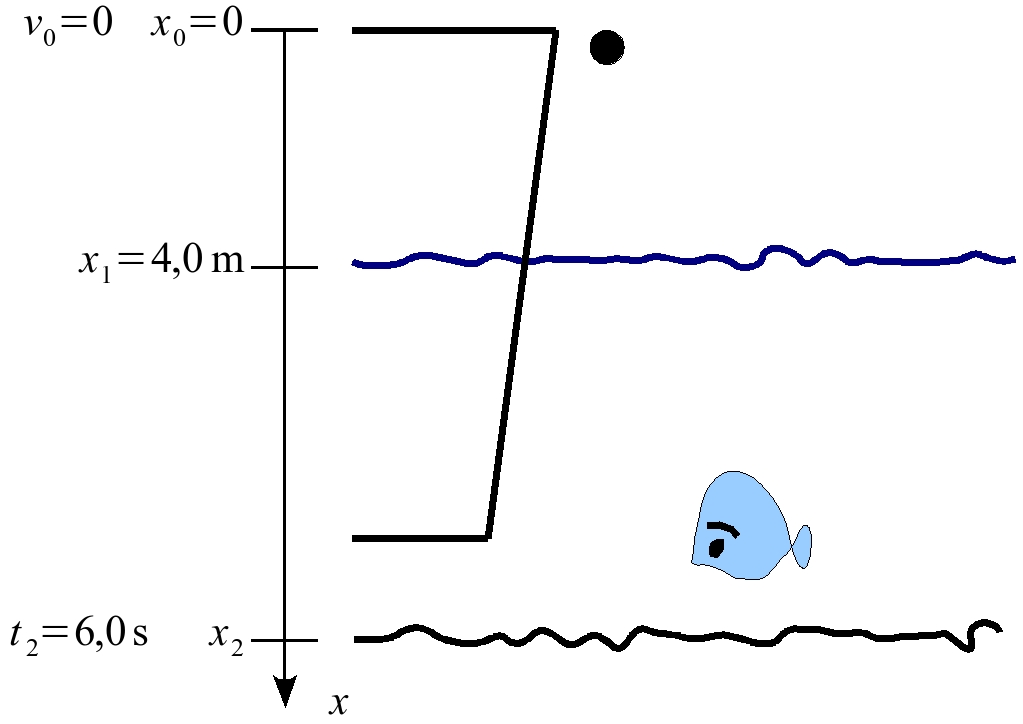
\includegraphics[width=0.4\textwidth]{boordschip}
\end{figure}
Omdat we weten hoe ver de bol moet vallen voordat hij het wateroppervlak bereikt, kunnen we zowel de tijd die de bol hiervoor nodig heeft als de snelheid waarmee de bol het wateroppervlak raakt, bepalen. We kiezen een as naar beneden zodat -- omdat de snelheid in deze richting toeneemt -- de versnelling positief is en gelijk aan de valversnelling $g$ (toch voor het eerste stuk). De beginsnelheid van de bol is nul omdat hij vanuit rust wordt losgelaten. Voor de tijd vinden we:
\begin{eqnarray}
x_1=\frac{1}{2}gt^2\quad\Rightarrow\quad t_1&=&\sqrt{\frac{2x_1}{g}}\label{tijd_boordschip}
\end{eqnarray}
Met de tijd\footnote{We zouden de tijd met het gevonden formuletje kunnen uitrekenen en met het getalletje dat we vinden verder rekenen. Maar met het formuletje verder werken -- algebra\"isch of symbolisch -- is toch o zo veel knapper en van toepassing voor \'alle boten en niet enkel voor een boot waarvoor het dek zich $4,0$ meter boven het wateroppervlak bevindt. Bovendien is het ``echte'' fysica omdat je een ``model'' uitwerkt en niet een rekensommetje oplost...} kunnen we de snelheid op het wateroppervlak vinden.
\begin{eqnarray}
v_1=gt_1\nonumber=g\sqrt{\frac{2x_1}{g}}\nonumber=\sqrt{2gx_1}\label{snelheid_boordschip}
\end{eqnarray}
Onder water, in het tweede stuk, beweegt de kogel met deze snelheid gedurende de resterende tijd: $6,0$ seconden min de tijd $t_1$ (\ref{tijd_boordschip}) die de kogel nodig had om te vallen. De afstand die de bol onder water aflegt, vinden we met de eenvoudige formuletjes van een ERB\footnote{Opmerking, een ERB is een speciaal geval van een EVRB. Een ERB heeft als constante versnelling $a=0$.}. We substitueren ook vergelijkingen (\ref{tijd_boordschip}) en (\ref{snelheid_boordschip}).
\begin{eqnarray*}
\Delta x&=&\overline{v}\cdot\Delta t\\
&\Downarrow&\\
x_2-x_1&=&v_1(t_2-t_1)\\
&=&\sqrt{2gx_1}(t_2-\sqrt{\frac{2x_1}{g}})\\
&=&\sqrt{2gx_1}t_2-2x_1\\
&=&45\rm\,m
\end{eqnarray*}
De gemiddelde snelheid vinden we door de totale afgelegde weg te delen door de totale benodigde tijd. Andere formuletjes zoals $\overline{v}=\frac{v_1+v_2}{2}$ zijn niet van toepassing omdat het helemaal niet over \'e\'en EVRB gaat waar dit formuletje geldt omdat de snelheid mooi lineair toeneemt. Hier gebeurt dat enkel in het eerste stuk en worden de verschillende snelheden niet even lang aangehouden zodat ze een verschillend aandeel hebben in de totale benodigde tijd.
\begin{eqnarray*}
\overline{v}_{02}=\frac{\Delta x}{\Delta t}=\frac{x_2}{t_2}&=&\frac{\sqrt{2gx_1}t_2-x_1}{t_2}\\
&=&\sqrt{2gx_1}-\frac{x_1}{t_2}\\
&=&8,2\rm\,m/s
\end{eqnarray*}}
\end{enumerate}

\cleardoublepage
\newpage
%!TEX root = ../cursus_fys6.tex
\chapter{Tweedimensionale bewegingen}

Als we in een vlak bewegen, hebben we te maken met een tweedimensionale beweging. 
Om ze te beschrijven voeren we nu een referentiestelsel met twee assen in. In de regel kiezen we een cartesiaans assenstelsel.  Door de co\"ordinaten $(x,y)$ van een punt dat het bewegende object voorstelt te geven, kunnen we de positie beschrijven. We kunnen echter ook een vector gebruiken.
\begin{figure}[h]
\centering
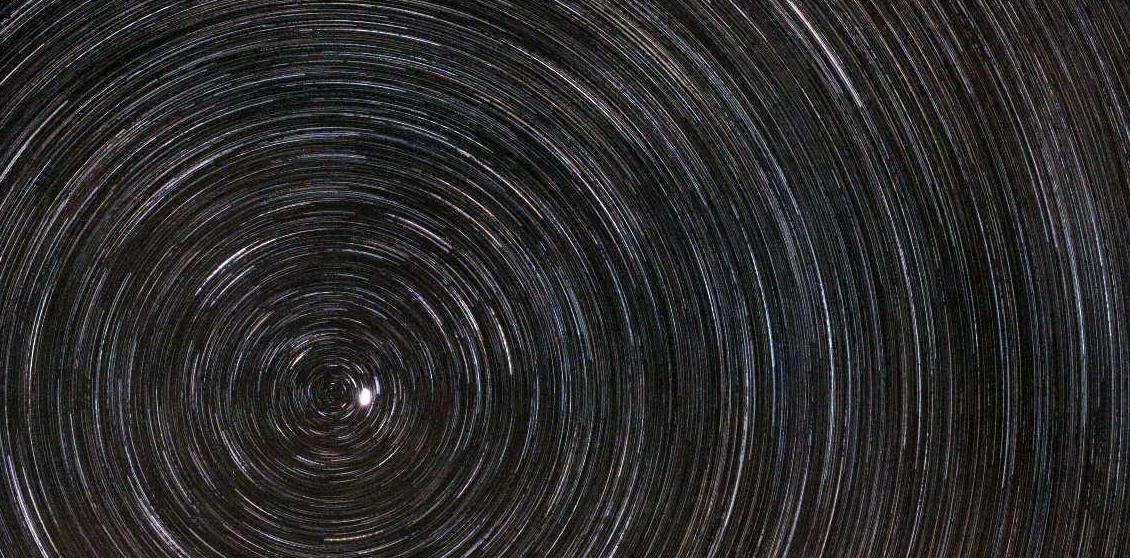
\includegraphics[width=.7\textwidth]{sterrentrajecten}
\caption{Sterrentrajecten aan de hemel}
\end{figure}
Omdat we om de snelheid van het object te kunnen beschrijven niet voldoende hebben aan alleen maar de grootte maar ook nood hebben aan een richting, maken we nu expliciet gebruik van vectoren en hun geschikte eigenschappen. Naast een nieuwe as voor de extra dimensie is het gebruik van vectoren de enige aanpassing die we aan ons formalisme van de kinematica moeten doen om bewegingen in twee dimensies te kunnen beschrijven.

\section{Onafhankelijkheidsbeginsel}

Stel je voor dat het heel mooi weer is. Zo van dat weer waar de hemel hemelsblauw is, er geen wolken aan de lucht zijn, de zon aan de hemel schittert en je niets liever doet dan een frisse neus halen. In zo'n weer zouden we diep in en uit ademen. Oh ja, detail, stel je ook voor dat er \emph{geen}\footnote{Begrijpelijk zou je kunnen opwerpen dat het nogal moeilijk is om frisse lucht die er niet is, in te ademen.} lucht is. Stel je bovendien voor dat je in het kraaiennest van een piratenschip zit. Het schip vaart met een gestadige, grote en constante snelheid over het zee-oppervlak dat geen enkele rimpeling vertoont. Golven zijn er niet\footnote{Ook hier zou je kunnen opperen dat een zee zonder golven niet echt een zee is.}. Stel je ook voor dat je een nogal zware kogel naar je uitkijkpost hebt meegenomen\footnote{Tja, in een gedachte-experiment zoals dit is veel mogelijk.}. Als je nu deze kogel laat vallen, met zicht op het achtersteven van het schip, dan \ldots dan valt hij natuurlijk regelrecht naar beneden op het hoofd van de kapitein die aan de voet van de mast staat en waarvoor me het arsenaal bijvoeglijke naamwoorden om zijn onuitstaanbaarheid te kunnen uitdrukken, even ontbreekt. Stel je nu ook voor dat zogezegd door de snelheid van het schip de kogel \emph{achter} het schip zou terechtkomen\footnote{Jawel, er zijn er onder ons die zich dat voorstellen} \ldots, dan zouden in een snel rijdende trein de valiezen die je op het rek legt zich met een enorme snelheid naar de achterkant van de wagon begeven, de kaarten die je wilt afleggen eveneens dezelfde plaats opzoeken i.p.v. netjes op de  aflegstapel te blijven liggen en dan zou de dame van de koffiebar enig kuiswerk hebben met de koffie die een ware ravage zou aanrichten \ldots 
\begin{figure}[h]
\centering
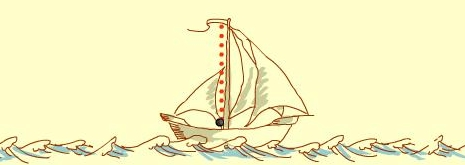
\includegraphics[height=2.3cm]{galileo_projectiles1} 
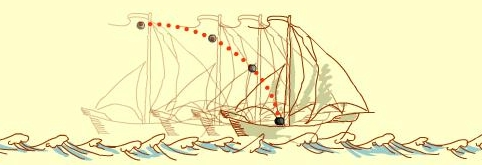
\includegraphics[height=2.3cm]{galileo_projectiles2} 
\caption{Dezelfde beweging van een kogel gezien door een waarnemer op het schip en een waarnemer buiten het schip.}
\end{figure}
Conclusie? Wel, de conclusie is enerzijds dat door de traagheid de kogel tijdens de val zijn snelheid vooruit, volgens de beweging van het schip, behoudt en recht op de kapitein terechtkomt en anderzijds dat de tijd die de kogel nodig heeft om in het luchtledige op de grond terecht te komen, onafhankelijk is van de snelheid die de kogel al dan niet meekrijgt in horizontale richting. De beweging van de kogel is immers voor iemand op het schip een verticale valbeweging en voor een buitenstaander een horizontale worp. Maar in beide gevallen gaat het om dezelfde beweging en dus ook over dezelfde benodigde tijd.\footnote{Mooie animatie: \url{http://www.pbs.org/wgbh/nova/galileo/expe_flash_2.html}}

\section{Enkele begrippen}

\subsection{Plaats, verplaatsing, afgelegde weg}

Om aan een vectori\"ele snelheid te komen, voeren we een plaatsvector $\vec{r}$ in. Deze kan van de tijd afhangen en kunnen we met behulp van de eenheidsvectoren $\vec{e}_x$ en $\vec{e}_y$ schrijven als
\begin{equation*}
 \vec{r}=x\cdot\vec{e}_x+y\cdot\vec{e}_y.
\end{equation*}
De tijdsafhankelijkheid kunnen we expliciet weergeven door $x(t)$ en $y(t)$ te gebruiken i.p.v. $x$ en $y$. De functies $x(t)$ en $y(t)$ noemen we de \emph{co\"ordinaat\-functies}. Door de plaats met een vector te beschrijven, kunnen we het begrip verplaatsing $\Delta x$ ook gemakkelijk en analoog uitbreiden naar twee dimensies. De verplaatsing
\begin{equation*}
\Delta\vec{r}=\vec{r}_2-\vec{r}_1
\end{equation*}
is nu immers ook een vector die naast de afstand in vogelvlucht tussen twee punten, ook ge\"ori\"enteerd is. Het is natuurlijk belangrijk in welke richting die afstand wordt afgelegd.
\begin{figure}[h]
\centering
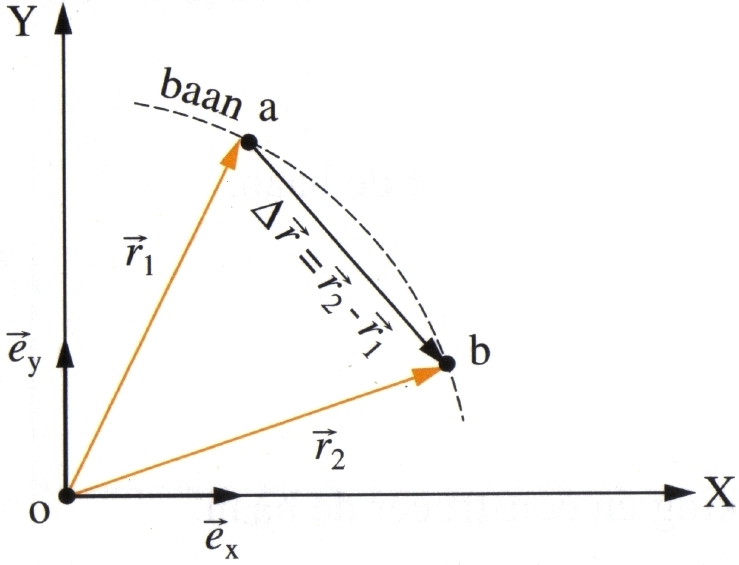
\includegraphics[width=0.4\textwidth]{plaatsvector}
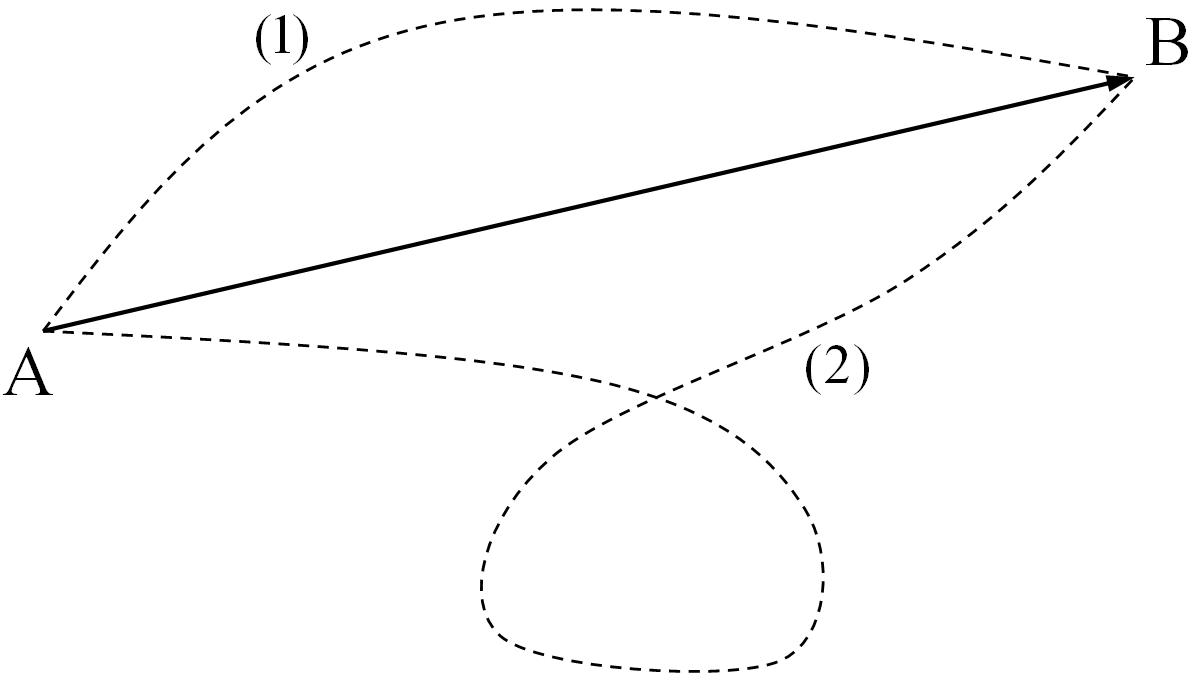
\includegraphics[width=0.4\textwidth]{afgelegdeweg_verplaatsing}
\caption{Het verschil tussen afgelegde weg en verplaatsing}
\end{figure}
Merk op dat de begrippen verplaatsing en afgelegde weg niet hetzelfde zijn. De afgelegde weg hangt af van de gevolgde baan en is de totale afgelegde afstand terwijl de verplaatsing enkel van begin- en eindpunt afhangt en een vectorgrootheid is.

Naast de co\"ordinaatfuncties $x(t)$ en $y(t)$ is er ook de vergelijking van de baan $y(x)$. We bekomen deze door de tijd uit de co\"ordinaatfuncties te elimineren\footnote{Dit komt neer op de inverse $t(x)$ van $x(t)$ te vinden en deze te substitueren in $y(t)$. Dus $y(x)=y(t(x))$.}. De grafiek van deze baanvergelijking geeft ons het beeld van de baan maar zegt niets over de snelheid waarmee het object over deze baan beweegt. Daarvoor hebben we de afhankelijkheid van de tijd nodig.

\subsection{Snelheid}

%\begin{wrapfigure}[9]{R}{0.35\textwidth}
%\centering
%\includegraphics[width=0.34\textwidth]{snelheidsvector}
%\end{wrapfigure}
Analoog aan de snelheid in \'e\'en dimensie, kunnen we in meerdere dimensies de snelheid defini\"eren als de afgeleide -- nu van de plaatsvector. De snelheid is dan opnieuw een vector:\footnote{De definitie van een afgeleide van een vector is evenzeer met een limiet. We maken gebruik van de uitdrukkingen $\vec{r}(t+\Delta t)=x(t+\Delta t)\vec{e}_x+y(t+\Delta t)\vec{e}_y$ en $\vec{r}(t)=x(t)\vec{e}_x+y(t)\vec{e}_y$.\begin{eqnarray*}
\vec{v}=\frac{d\vec{r}}{dt}&=&\lim_{\Delta t\to 0}\frac{\vec{r}(t+\Delta t)-\vec{r}(t)}{\Delta t}\\
&=&\lim_{\Delta t\to 0}\frac{[x(t+\Delta t)\vec{e}_x+y(t+\Delta t)\vec{e}_y]-[x(t)\vec{e}_x+y(t)\vec{e}_y]}{\Delta t}\\
&=&\lim_{\Delta t\to 0}\frac{[x(t+\Delta t)-x(t)]\vec{e}_x+[y(t+\Delta t)-y(t)]\vec{e}_y}{\Delta t}\\
&=&\lim_{\Delta t\to 0}\left(\frac{x(t+\Delta t)-x(t)}{\Delta t}\right)\vec{e}_x+\lim_{\Delta t\to 0}\left(\frac{y(t+\Delta t)-y(t)}{\Delta t}\right)\vec{e}_y\\
&=&\frac{dx}{dt}\vec{e}_x+\frac{dy}{dt}\vec{e}_y%\\&=&v_x\vec{e}_x+v_y\vec{e}_y
\end{eqnarray*}}
\begin{eqnarray*}
\vec{v}=\frac{d\vec{r}}{dt}=\frac{d}{dt}\left(x\cdot\vec{e}_x+y\cdot\vec{e}_y\right)=\frac{dx}{dt}\vec{e}_x+\frac{dy}{dt}\vec{e}_y%=v_x\vec{e}_x+v_y\vec{e}_y
\end{eqnarray*}
De eenheidsvectoren $\vec{e}_x$ en $\vec{e}_y$ veranderen niet in de tijd zodat we die buiten de afgeleide hebben kunnen brengen. We zien dat de snelheidsvector dus te ontbinden is in componenten waarbij de componenten gewoonweg de snelheden van de afzonderlijke co\"ordinaten zijn. 
\begin{eqnarray*}
\vec{v}=v_x\vec{e}_x+v_y\vec{e}_y\quad\mathrm{met}\quad v_x=\frac{dx}{dt},\,v_y=\frac{dy}{dt}
\end{eqnarray*}

%\begin{figure}[h]
%\centering
%%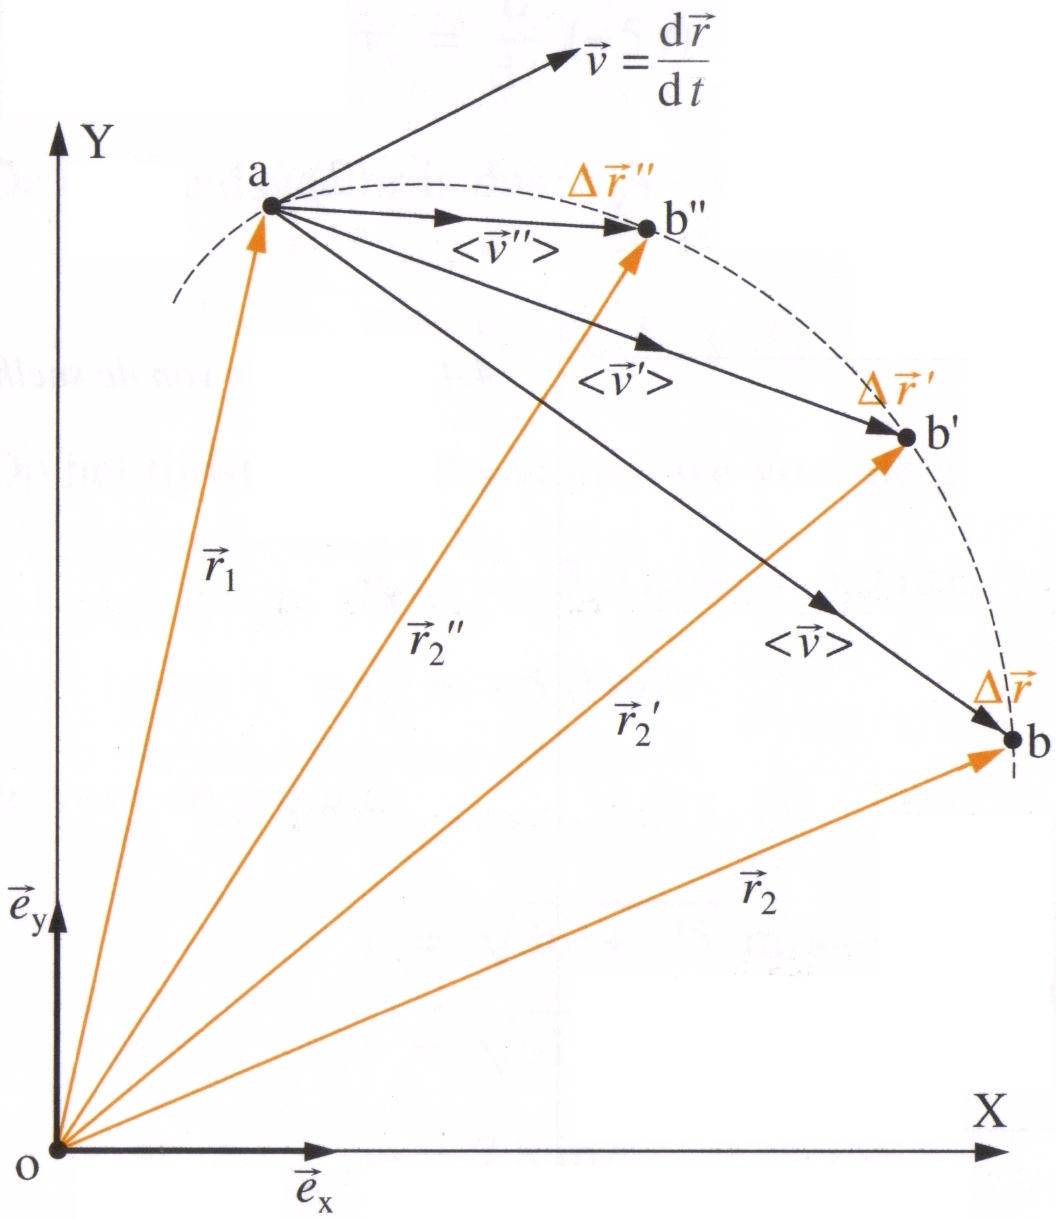
\includegraphics[width=0.38\textwidth]{gem_snelheidsvector}
%%\hspace{1cm}
%\includegraphics[width=0.4\textwidth]{snelheidsvector}
%\caption{De snelheidsvector is te ontbinden in componenten}
%\end{figure}
%\newline

\newpage

\begin{eigenschap}
De snelheidsvector is rakend aan de baan.
\end{eigenschap}
%\begin{figure}[h]
%\centering
%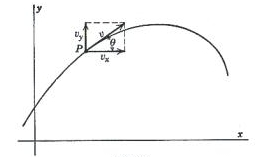
\includegraphics[width=0.4\textwidth]{snelheidrakend}
%\caption{De snelheid raakt aan de baan}
%\end{figure}
\begin{proof}
We kunnen dit bewijzen met de kettingregel, toegepast op de functie $y(t)=y(x(t))$.
\begin{eqnarray*}
 \frac{dy}{dt}=\frac{dy}{dx}\frac{dx}{dt}\Leftrightarrow\frac{dy}{dx}=\frac{\frac{dy}{dt}}{\frac{dx}{dt}}=\frac{v_y}{v_x}
\end{eqnarray*}
Inderdaad, $\frac{dy}{dx}$ is de helling van de baan en deze valt samen met de helling die de snelheidsvector maakt $\frac{v_y}{v_x}$.
\end{proof}

\subsection{Versnelling}

Ook de versnelling definieren we analoog; als afgeleide van de snelheid.
\begin{eqnarray*}
\vec{a}=\frac{d\vec{v}}{dt}=\frac{dv_x}{dt}\vec{e}_x+\frac{dv_y}{dt}\vec{e}_y=a_x\vec{e}_x+a_y\vec{e}_y
\end{eqnarray*}
Merk op dat er een versnelling kan zijn wanneer de snelheidsvector van grootte verandert maar \'o\'ok wanneer de snelheidsvector van richting verandert! Als de snelheidsvector immers van richting verandert, veranderen zijn co\"ordinaten $v_x$ en/of $v_y$. Merk bovendien op dat de versnelling niet noodzakelijk samen hoeft te vallen met de baan \ldots
\begin{figure}[h]
\centering
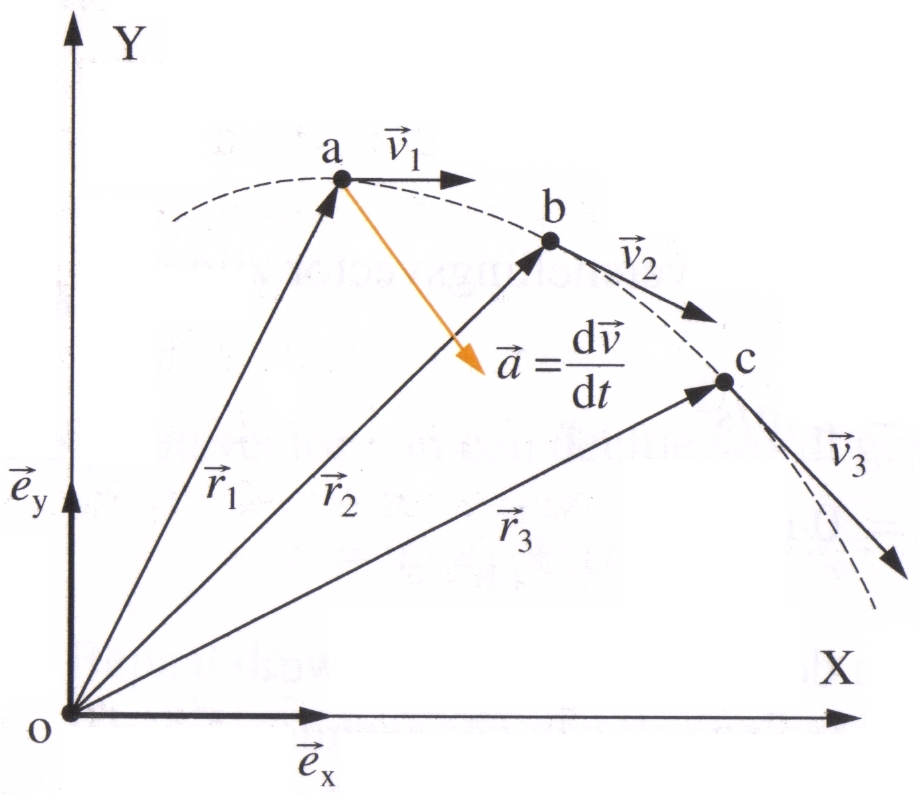
\includegraphics[width=0.4\textwidth]{versnellingsvector}
\caption{De versnelling raakt niet noodzakelijk aan de baan}
\end{figure}

\newpage

%oefening baanvergelijking, enz.

\begin{enumerate}
\item[\textbf{Opdracht}]\textsf{De positie van een deeltje als functie van de tijd wordt beschreven door
\begin{displaymath}
\vec{r}=bt\vec{e}_x+(c-dt^2)\vec{e}_y
\end{displaymath}
met $b=2,00\rm\,m/s$, $c=5,00\rm\,m$ en $d=1,00\rm\,m/s^2$.
\begin{enumerate}
\item Druk $y$ uit in functie van $x$. Hoe ziet de baan eruit?
\item Bepaal de snelheidsvector.
\item Op welk tijdstip ($t>0$) staat de snelheid loodrecht op de plaatsvector?
\end{enumerate}
\item[\textit{oplossing}]
\begin{enumerate}
\item We moeten dus de baanvergelijking geven. Dit doen we door de tijd uit te drukken i.f.v. de positie $x$ en dit te substitueren in de co\"ordinaatvergelijking $y(t)$.
\begin{eqnarray*}
x&=&bt\Leftrightarrow t=\frac{x}{b}\\
&\Downarrow&\\
y&=&c-dt^2=c-\frac{d}{b^2}x^2
\end{eqnarray*}
Dit is een bergparabool met top $(0,c)=(0,5,00\rm\,m)$
\item De componenten van de snelheid zijn:
\begin{eqnarray*}
v_x&=&\frac{dx}{dt}=b\\
v_y&=&\frac{dy}{dt}=-2dt
\end{eqnarray*}
zodat de snelheid(svector) wordt gegeven door
\begin{eqnarray*}
\vec{v}&=&v_x\vec{e}_x+v_y\vec{e}_y\\
&=&b\vec{e}_x-2dt\vec{e}_y
\end{eqnarray*}
\item De rechte die de richting van de snelheid weergeeft, staat loodrecht op de rechte die de richting van de positievector weergeeft wanneer het product van de richtingsco\"effici\"enten gelijk is aan $-1$:
\begin{eqnarray*}
rc_{r}\cdot rc_{v}&=&-1\\
&\Updownarrow&\\
\frac{y}{x}\cdot\frac{v_y}{v_x}&=&-1\\
&\Downarrow&\\
\frac{c-dt^2}{bt}\cdot\frac{-2dt}{b}&=&-1\\
&\Downarrow&(t>0)\\
t&=&\sqrt{\frac{2cd-b^2}{2d^2}}\\
&=&1,73\rm\,s
\end{eqnarray*}
\end{enumerate}}
\end{enumerate}

\newpage

\section{De eenparige cirkelbeweging}

De cirkelbeweging is op het eerste zicht misschien een zeer eenvoudige beweging maar wel alom tegenwoordig. Denk maar aan een tolbeweging, een kermisattractie zoals een carrousel, wielen, planeetbanen of aan het nemen van een bocht met de auto of de fiets. Vandaar dat het een toch een erg belangrijke beweging is. Wij bestuderen een eenparige cirkelbeweging (ECB). Dat betekent dat de baan van het object een cirkel is en dat de grootte van de snelheid waarmee de baan wordt doorlopen, constant is.

\subsection{Enkele begrippen}

Om een cirkelbeweging te beschrijven, hebben we enkele begrippen nodig die je eventueel nog onbekend zijn. Zo is er de \emph{frequentie}. Het is algemeen het aantal trillingen of cyclussen van een periodieke beweging die per seconde worden doorlopen. Specifiek voor de cirkelbeweging is de frequentie dan het aantal keren dat de cirkel doorlopen wordt per tijdseenheid. De frequentie krijgt het symbool $f$ en heeft als eenheid de Hertz, $[f]=\rm Hz=s^{-1}$. Het begrip \emph{periode} gebruiken we voor de tijdsduur die nodig is voor het doorlopen van \'e\'en cyclus. Het symbool is $T$ en de eenheid seconde, $[T]=s$. Het aantal cyclussen dat in de periode wordt doorlopen is \'e\'en zodat de volgende relatie tussen de frequentie en de periode bestaat.
\begin{equation*}
f=\frac{1}{T}
\end{equation*}
Als laatste hebben we nog het begrip \emph{hoeksnelheid}. 
\begin{figure}[h]
\centering 
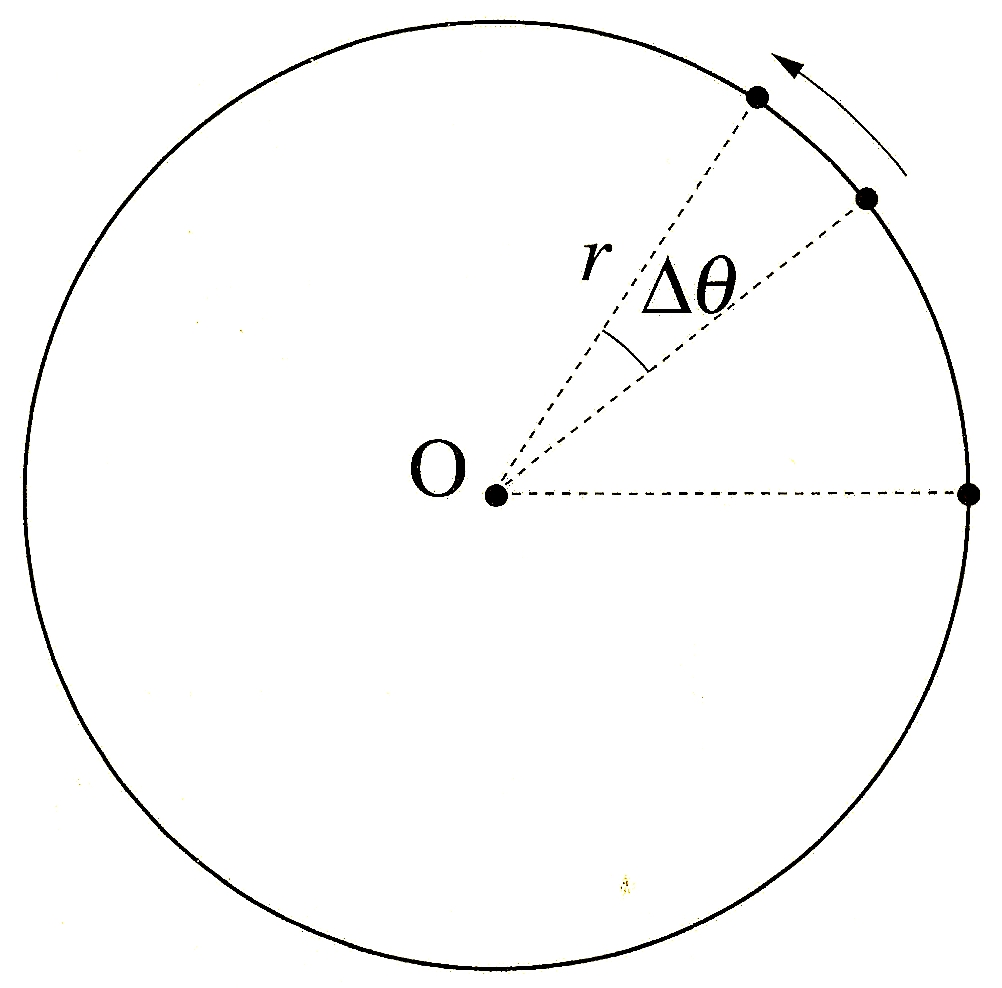
\includegraphics[width=0.35\textwidth]{ecb_hoeksnelheid}
\caption{De hoeksnelheid}
 % ecb_hoeksnelheid.jpg: 1002x988 pixel, 72dpi, 35.35x34.85 cm, bb=0 0 1002 988
\end{figure}
Verschillende punten op je fietswiel hebben verschillende snelheden als hun afstand tot het centrum verschilt. Het ventieldopje moet immers in eenzelfde tijd meer afstand afleggen dat het sensortje van je snelheidsmeter. Toch bestaat het wiel uit \'e\'en geheel. Als je naar de omwentelingshoek kijkt die een straal vanuit het centrum door een punt op het wile maakt, dan is die voor alle punten gelijk. Hoe sneller het wiel draait, hoe groter ook de omwentelingshoek is die een straal gemaakt heeft. Daarom defini\"eren we de hoeksnelheid $\omega$ als de verandering van de omwentelingshoek tot de benodigde tijd.\footnote{De letter $\omega$ is de kleine letter van $\Omega$ en de laatste letter in het Griekse alfabet. Spreek $\omega$ uit als omega. Een $\omega$ is geen w, zoals ook een w geen $\omega$ is. O wee ($\omega$?) als je je op het examen in juni vergist \ldots}
\begin{equation*}
\omega=\frac{\Delta\theta}{\Delta t}
\end{equation*}
De eeneid is radialen per seconde, $[\omega]=\rm rad/s$. Aangezien een volledige omwentelingshoek $2\pi$ bedraagt en de tijd nodig om rond te gaan de periode is, geldt
\begin{equation}
\omega=\frac{2\pi}{T}=2\pi f\label{hoeksnelheid}
\end{equation}

\subsection{Kinematica van de cirkelbeweging}

We beschouwen een punt dat een cirkelbeweging maakt met straal $r$. We voeren een assenstelsel in met de oorsprong in het middelpunt van de cirkel. 
\begin{figure}[h]
\centering
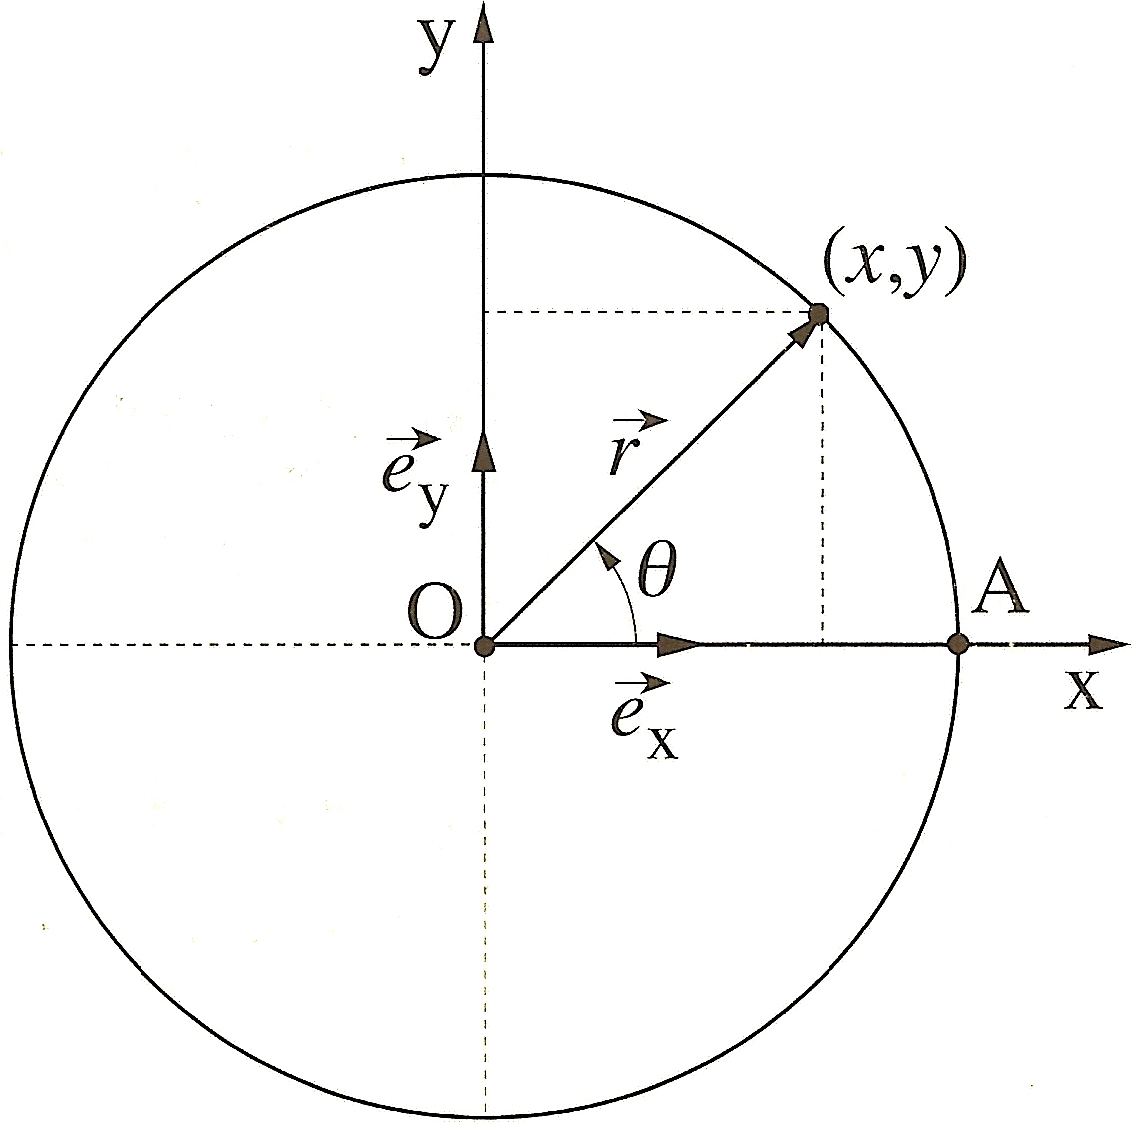
\includegraphics[width=0.4\textwidth]{ecb_positie}
\caption{Co\"ordinaten}
\end{figure}
Als we de omwentelingshoek $\theta$ meten vanaf de positieve $x$-as en en het tijdstip $t_0=0$ nemen, kunnen we de doorlopen omwentelingshoek als volgt in functie van de tijd schrijven.
\begin{equation*}
\omega=\frac{\Delta\theta}{\Delta t}=\frac{\theta-\theta_0}{t-t_0}=\frac{\theta}{t}\quad\Rightarrow\quad\theta=\omega t
\end{equation*}
De co\"ordinaatfuncties vinden we dan als projecties op de $x$- en $y$-as.
\begin{eqnarray*}
x(t)&=&r\cos\omega t\\
y(t)&=&r\sin\omega t
\end{eqnarray*}
We krijgen dan voor de plaatsvector, de snelheid en de versnelling:
\begin{eqnarray}
\vec{r}&=&r\cos\omega t\cdot\vec{e}_x+r\sin\omega t\cdot\vec{e}_y\nonumber\\
&\Downarrow&
\left\{\begin{array}{l}
v_x=\frac{dx}{dt}=-\omega r\sin\omega t\\
v_y=\frac{dy}{dt}=\omega r\cos\omega t
\end{array}
\right.\nonumber\\
\vec{v}&=&-\omega r\sin\omega t\cdot\vec{e}_x+\omega r\cos\omega t\cdot\vec{e}_y\nonumber\\
&\Downarrow&
\left\{\begin{array}{l}
a_x=\frac{dv_x}{dt}=-\omega^2 r\cos\omega t\\
a_y=\frac{dv_y}{dt}=-\omega^2 r\sin\omega t
\end{array}
\right.\nonumber\\
\vec{a}&=&-\omega^2 r\cos\omega t\cdot\vec{e}_x-\omega^2 r\sin\omega t\cdot\vec{e}_y\nonumber\\
&=&-\omega^2(r\cos\omega t\cdot\vec{e}_x+r\sin\omega t\cdot\vec{e}_y)\nonumber\\
&\Updownarrow&\nonumber\\
\vec{a}&=&-\omega^2\vec{r}\label{versnelling}
\end{eqnarray}
Deze laatste gelijkheid is erg belangrijk. We vinden dat de versnelling steeds naar het middelpunt van de cirkel is ge\"ori\"enteerd \ldots! We noemen het bijgevolg een centripetale\footnote{Dit is niet hetzelfde als centrifugaal.} of middelpuntzoekende versnelling. 
\begin{figure}[h]
\centering
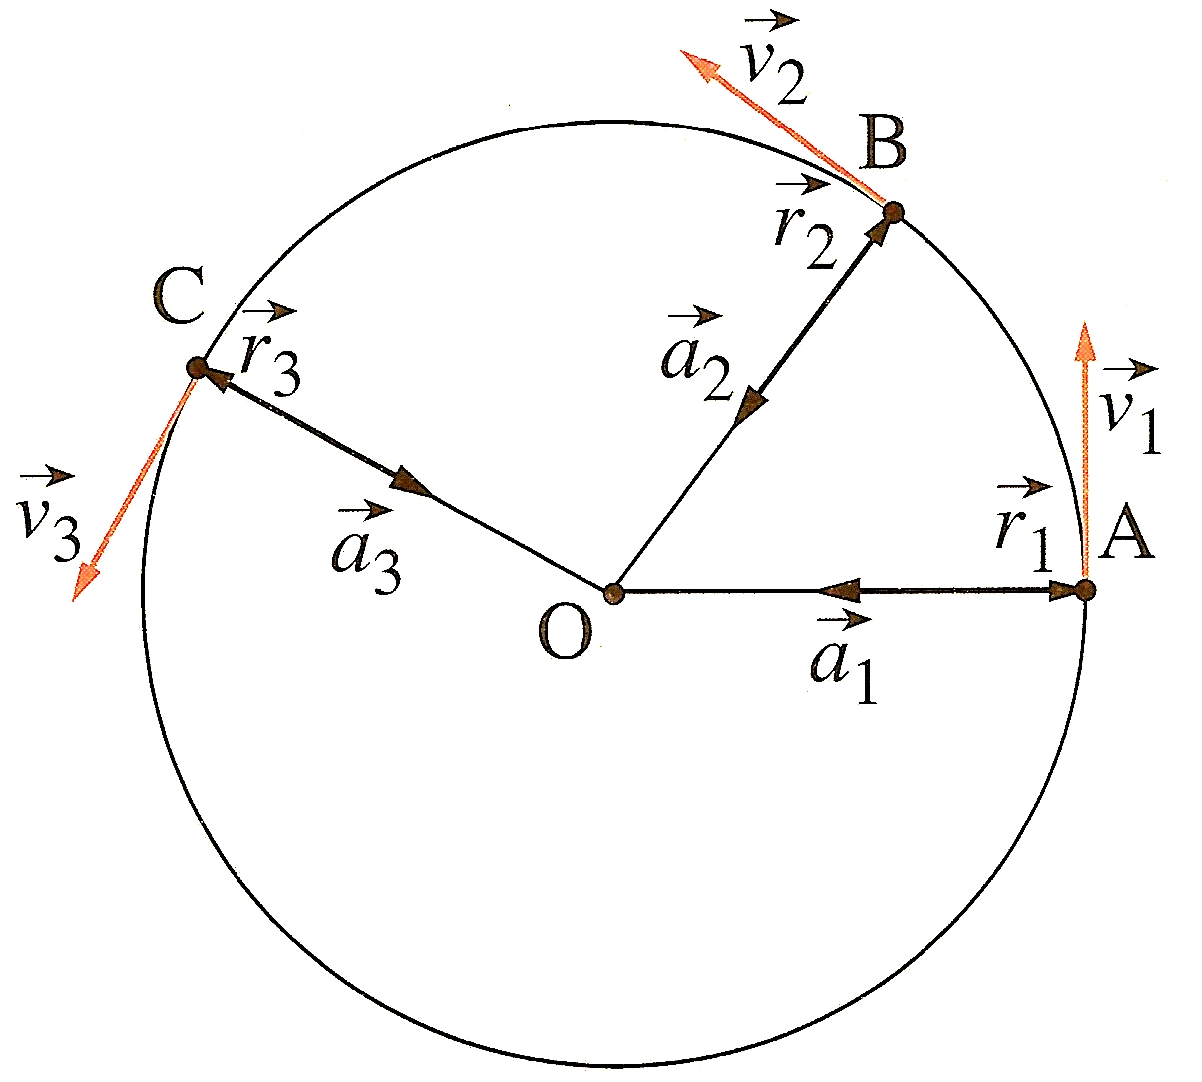
\includegraphics[width=0.4\textwidth]{ecb_versnelling}
\caption{De middelpuntzoekende versnelling}
\end{figure}
Je zou dit resultaat opmerkelijk kunnen noemen aangezien de snelheid een constante grootte heeft.
\begin{eqnarray}
v=\parallel\vec{v}\parallel&=&\sqrt{v_x^2+v_y^2}\nonumber\\
&=&\sqrt{(-\omega r\sin\omega t)^2+(\omega r\cos\omega t)^2}\nonumber\\
&=&\sqrt{r^2\omega^2(\sin^2\omega t+\cos^2\omega t)}\nonumber\\
&\Updownarrow&\nonumber\\
v&=&r\omega\label{snelheid}
\end{eqnarray}
Echter verandert de richting van de snelheid en aangezien de versnelling de verandering van de snelheid is, moet er een versnelling zijn. Deze is naar het centrum ge\"ori\"enteerd omdat een fractie van een seconde later het object -- in vergelijking met de baan die het zou afleggen moest het volgens de snelheid die het op een bepaald moment heeft, voortbewegen -- iets dichter naar het centrum moet zijn gekomen. De snelheidsvector is in grootte niet veranderd maar wel gedraaid, in de richting van het centrum. Moest bovendien de versnelling niet loodrecht op de snelheid staan, dan zou de versnelling een component volgens de snelheid hebben wat zou betekenen dat de snelheid in die richting zou moeten toenemen.
\begin{figure}[h]
\centering
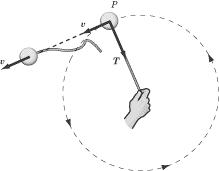
\includegraphics[width=0.4\textwidth]{ballnostring}
\caption{Moest er geen versnelling naar het centrum zijn -- bv. in het geval dat een touwtje met een ronddraaiend object aan, knapt -- dan zou de snelheid niet veranderen en het object op een rechte baan in het verlengde van de snelheid met een constante snelheid voortbewegen.}
\end{figure}

Uit (\ref{hoeksnelheid}), (\ref{versnelling}) en (\ref{snelheid}) vinden we nog:
\begin{equation}
a=r\omega^2=v\omega=\frac{v^2}{r}
\end{equation}
Merk op dat de snelheid een kwadratische invloed op de grootte van de versnelling heeft.

\newpage


\section{De horizontale worp}

We bekijken een voorbeeld van een tweedimensionale beweging. Wanneer een object horizontaal met een bepaalde beginsnelheid wordt gecatapulteerd, noemen we die beweging een horizontale worp. Wij beschouwen de worp in het luchtledige.
\begin{figure}[h]
\centering
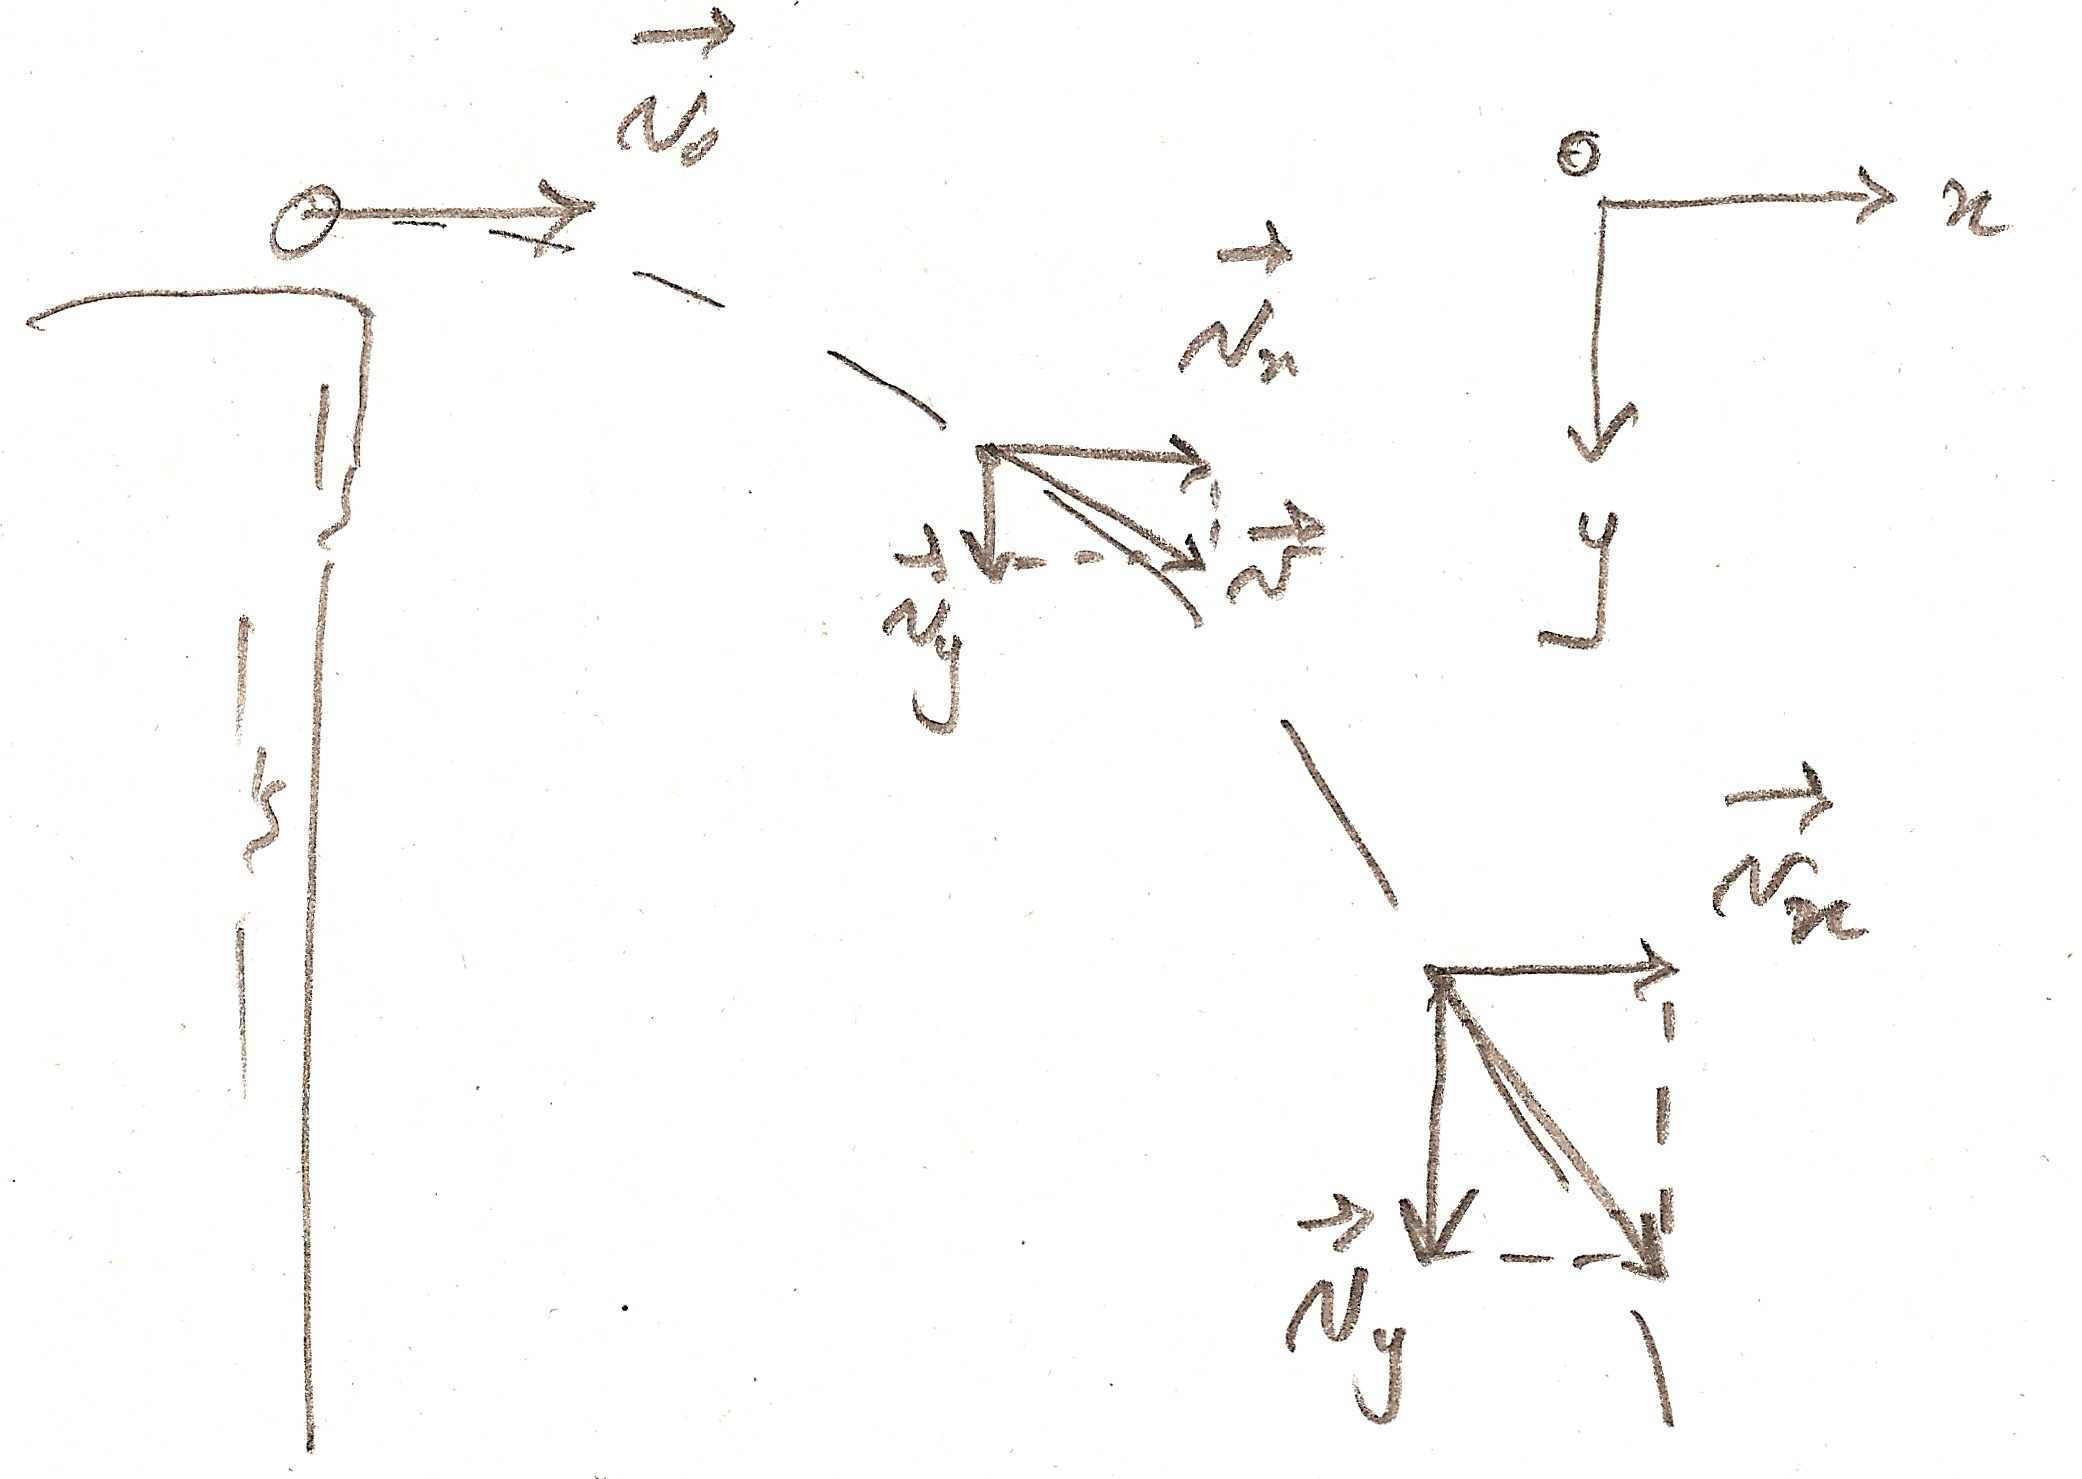
\includegraphics[width=0.6\textwidth]{horizontaleworp_tekening}
\caption{De snelheid in horizontale richting verandert niet, die in de verticale richting neemt lineair toe in de tijd}
\end{figure}
\newline
In de beschrijving kunnen we de $x$-as horizontaal en de $y$-as verticaal naar beneden nemen. Omdat er volgens de $x$-as geen versnelling is het lichaam volgens de $y$-as valt met de valversnelling $g$, kunnen we de formules voor een ERB en een EVRB (Zie (\ref{x(t)0}) en (\ref{v(t)0})) op de afzonderlijke assen toepassen en zo de volledige beweging beschrijven.%\footnote{Strikt genomen zoeken we hier nog niet naar een verklaring (die voor de horizontale beweging in de wet van de traagheid zit) maar beschrijven we enkel de beweging. Waarom de versnelling nul en $g$ is, vragen we ons dus zogezegd nog even niet af.}.
\begin{equation*}
\left\{
\begin{array}{l}
a_x=0\\
a_y=g
\end{array}
\right.
\Rightarrow
\left\{
\begin{array}{l}
v_x=v_0\\
v_y=gt
\end{array}
\right.
\Rightarrow
\left\{
\begin{array}{l}
x=v_0t\\
y=\frac{1}{2}gt^2
\end{array}
\right.
\end{equation*}
De baanvergelijking vinden we zoals eerder vermeld, door $t$ in functie van $x$ te schrijven $x=v_0t\Leftrightarrow t=\frac{x}{v_0}$ en dit in $y(t)$ te substitueren:
\begin{eqnarray*}
%&&x=v_0t\Leftrightarrow t=\frac{x}{v_0}\\
y=\frac{1}{2}gt^2=\frac{1}{2}g\left(\frac{x}{v_0}\right)^2=\frac{g}{2v_0^2}x^2
\end{eqnarray*}
De baan is dus een parabool.

\newpage

%oefening horizontale worp

\begin{enumerate}
\item[\textbf{Opdracht}]\textsf{Een vliegtuig vliegt met een snelheid van $450\rm\,km/h$ op een hoogte van $920\rm\,m$.
\begin{enumerate}
\item Hoever voor het doel moeten de voedselpakketten gelost worden
om op het doel terecht te komen?
\item Hoeveel tijd hebben de pakketten nodig om het doel te bereiken?
\end{enumerate}
\item[\textit{gegeven}]$v_0=125\rm\,m/s$\newline$y=920\rm\,m$
\item[\textit{gevraagd}]$x$, $t$
\item[\textit{oplossing}]De afstand waarover de voedselpakketten in
horizontale richting zijn vooruit gegaan, kunnen we vinden met de
baanvergelijking. We weten namelijk hoever de pakketten naar beneden
zijn gevallen en wat hun beginsnelheid is:
\begin{eqnarray*}
y&=&\frac{g}{2v_0^2}x^2\\
&\Downarrow&\\
x&=&v_0\sqrt{\frac{2y}{g}}=1712\rm\,m
\end{eqnarray*}
De valtijd voor de pakketten vinden we o.a. door naar de verticale
valbeweging te kijken. Deze gebeurt onafhankelijk van wat er in de
horizontale richting gebeurt, zodat:
\begin{eqnarray*}
y&=&\frac{1}{2}gt^2\\
&\Downarrow&\\
t&=&\sqrt{\frac{2y}{g}}=13,7\rm\,s
\end{eqnarray*}}
\end{enumerate}

\cleardoublepage
\newpage
\cleardoublepage
\null\thispagestyle{empty}

\vfill

\begin{center}
\textsc{DEEL II}
\end{center}
\begin{center}
\textsc{\LARGE DYNAMICA}
\end{center}

\vfill

\begin{figure}[h]
\centering
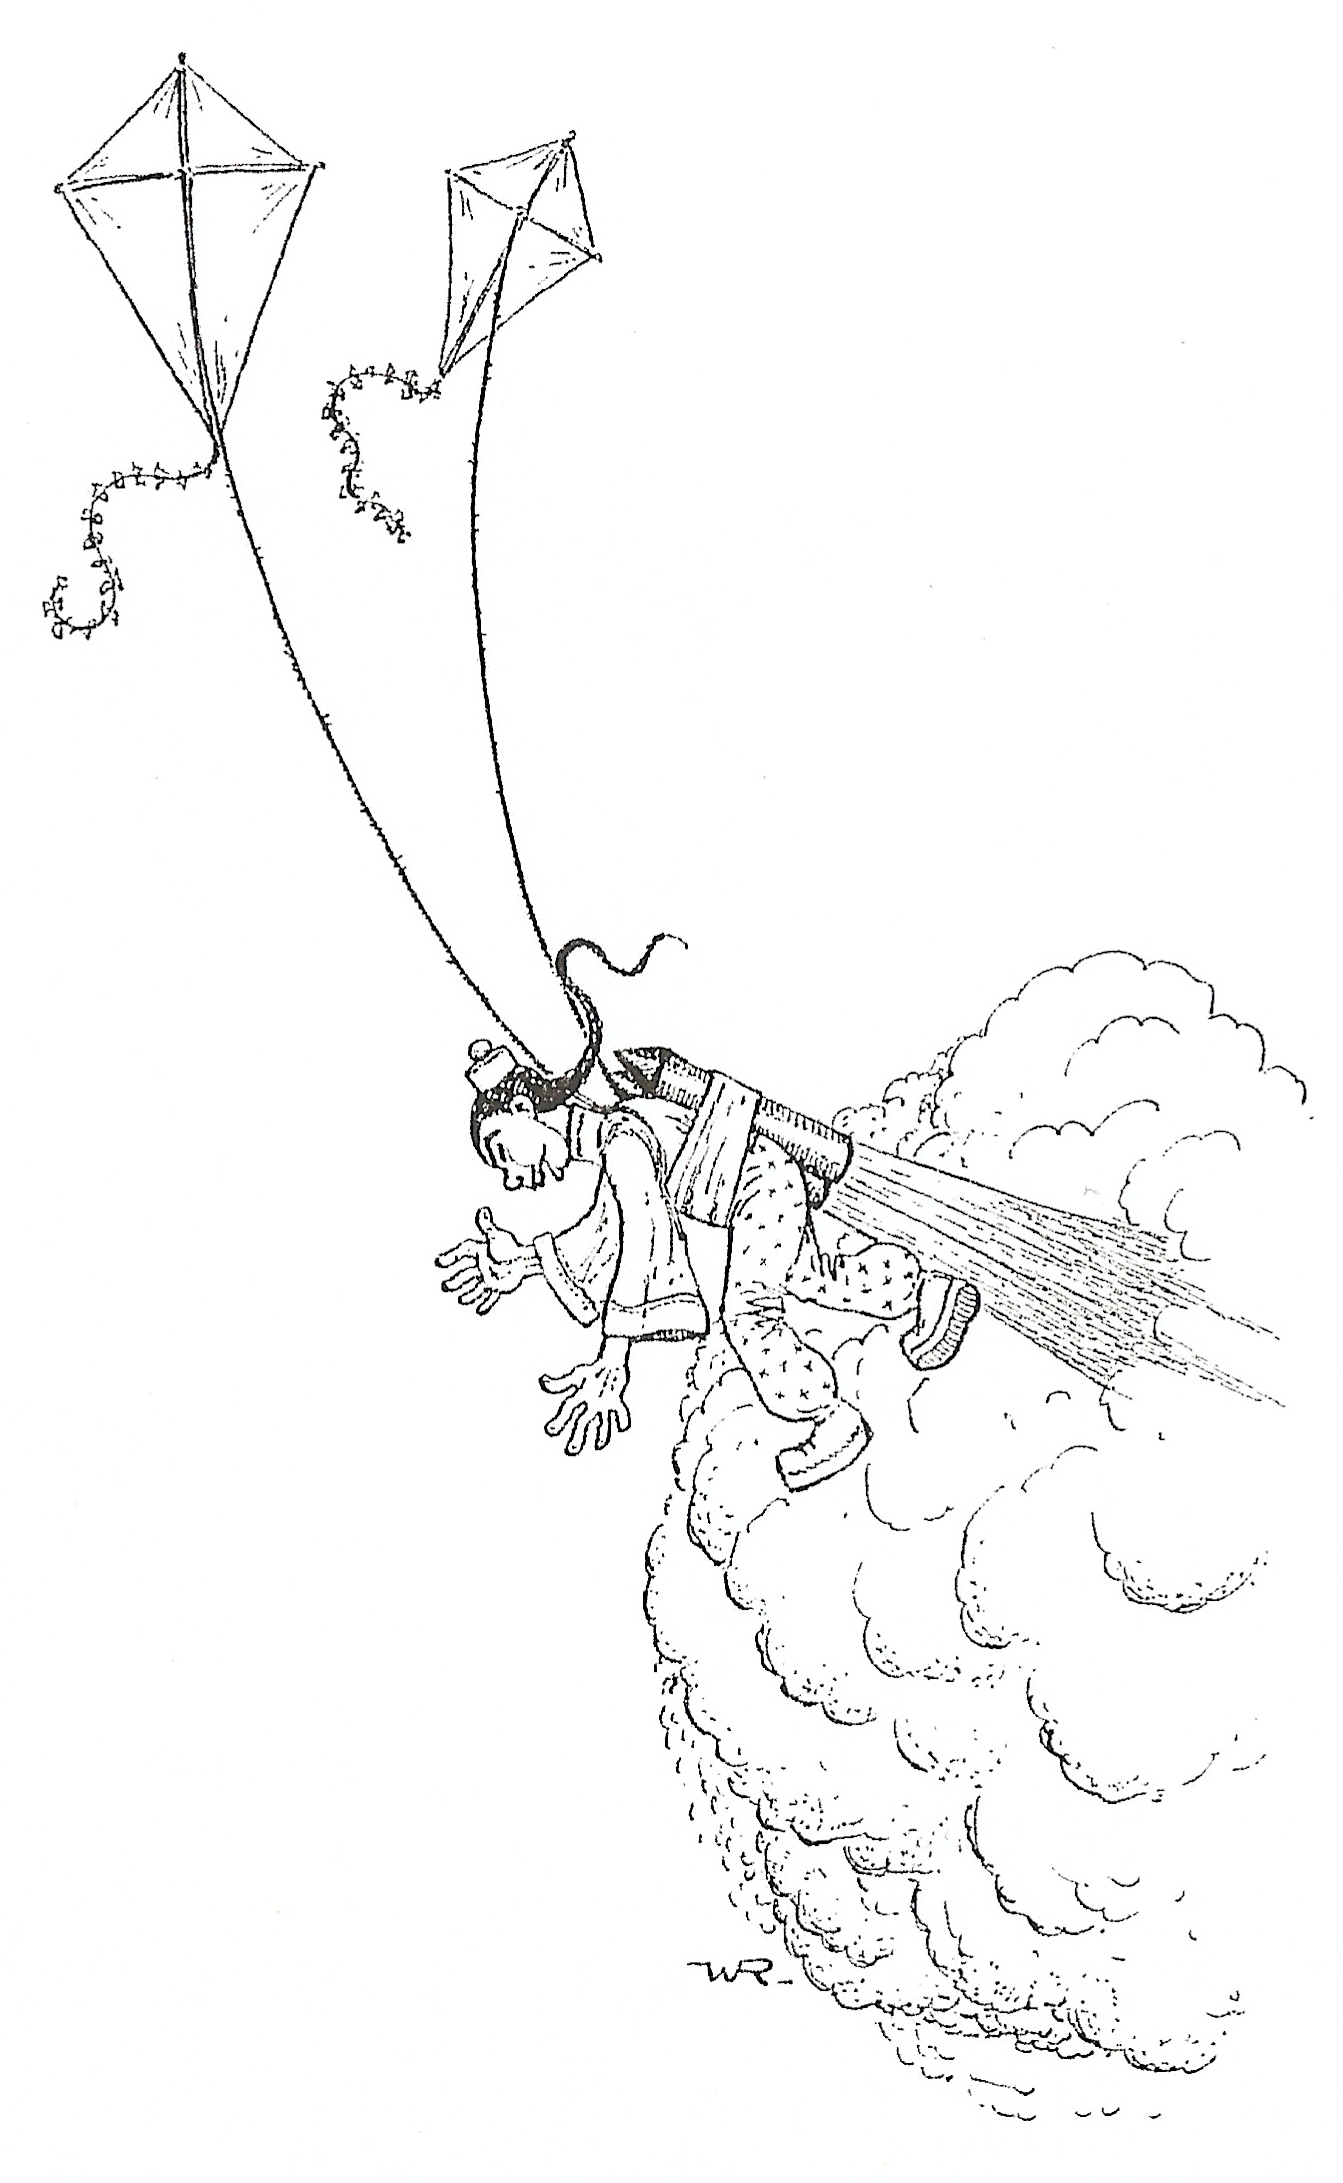
\includegraphics[width=0.65\textwidth]{raket_dynamica}
\end{figure}

%\begin{center}
%\begin{picture}(90,120)(0,0)
%%\put(115,0){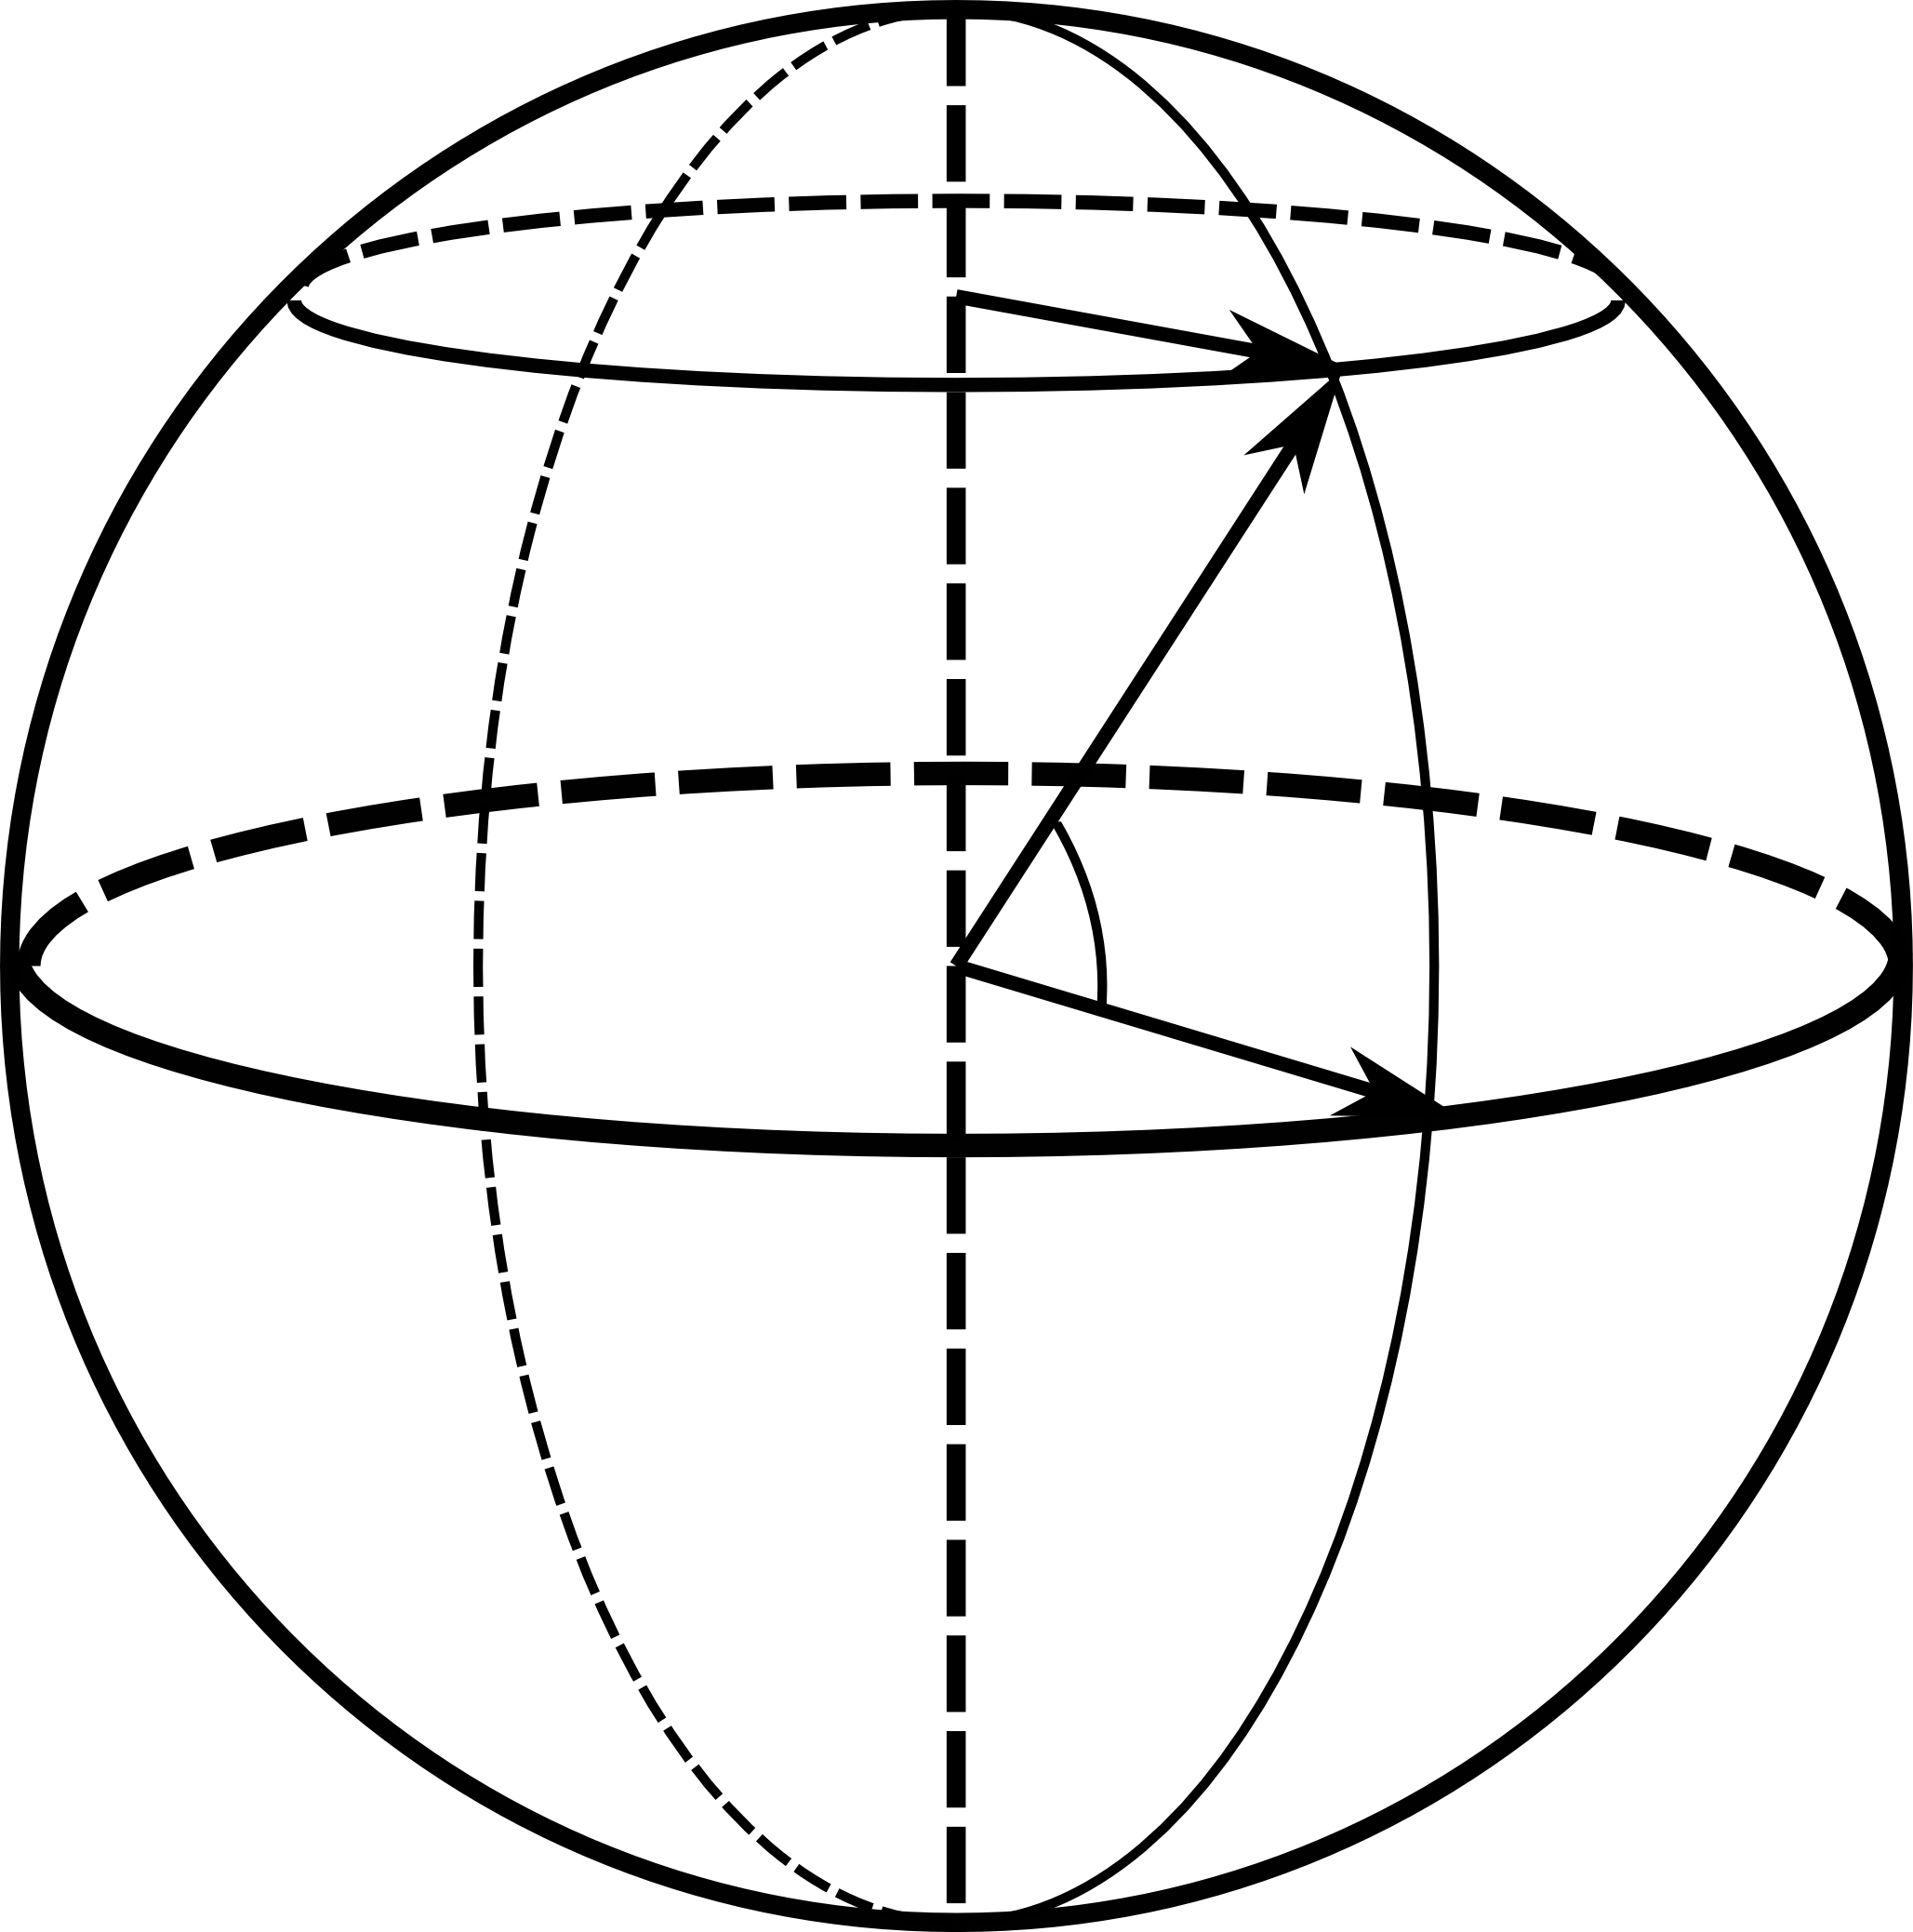
\includegraphics[scale=1.0]{aardehoeksnelheid}}
%\put(10,0){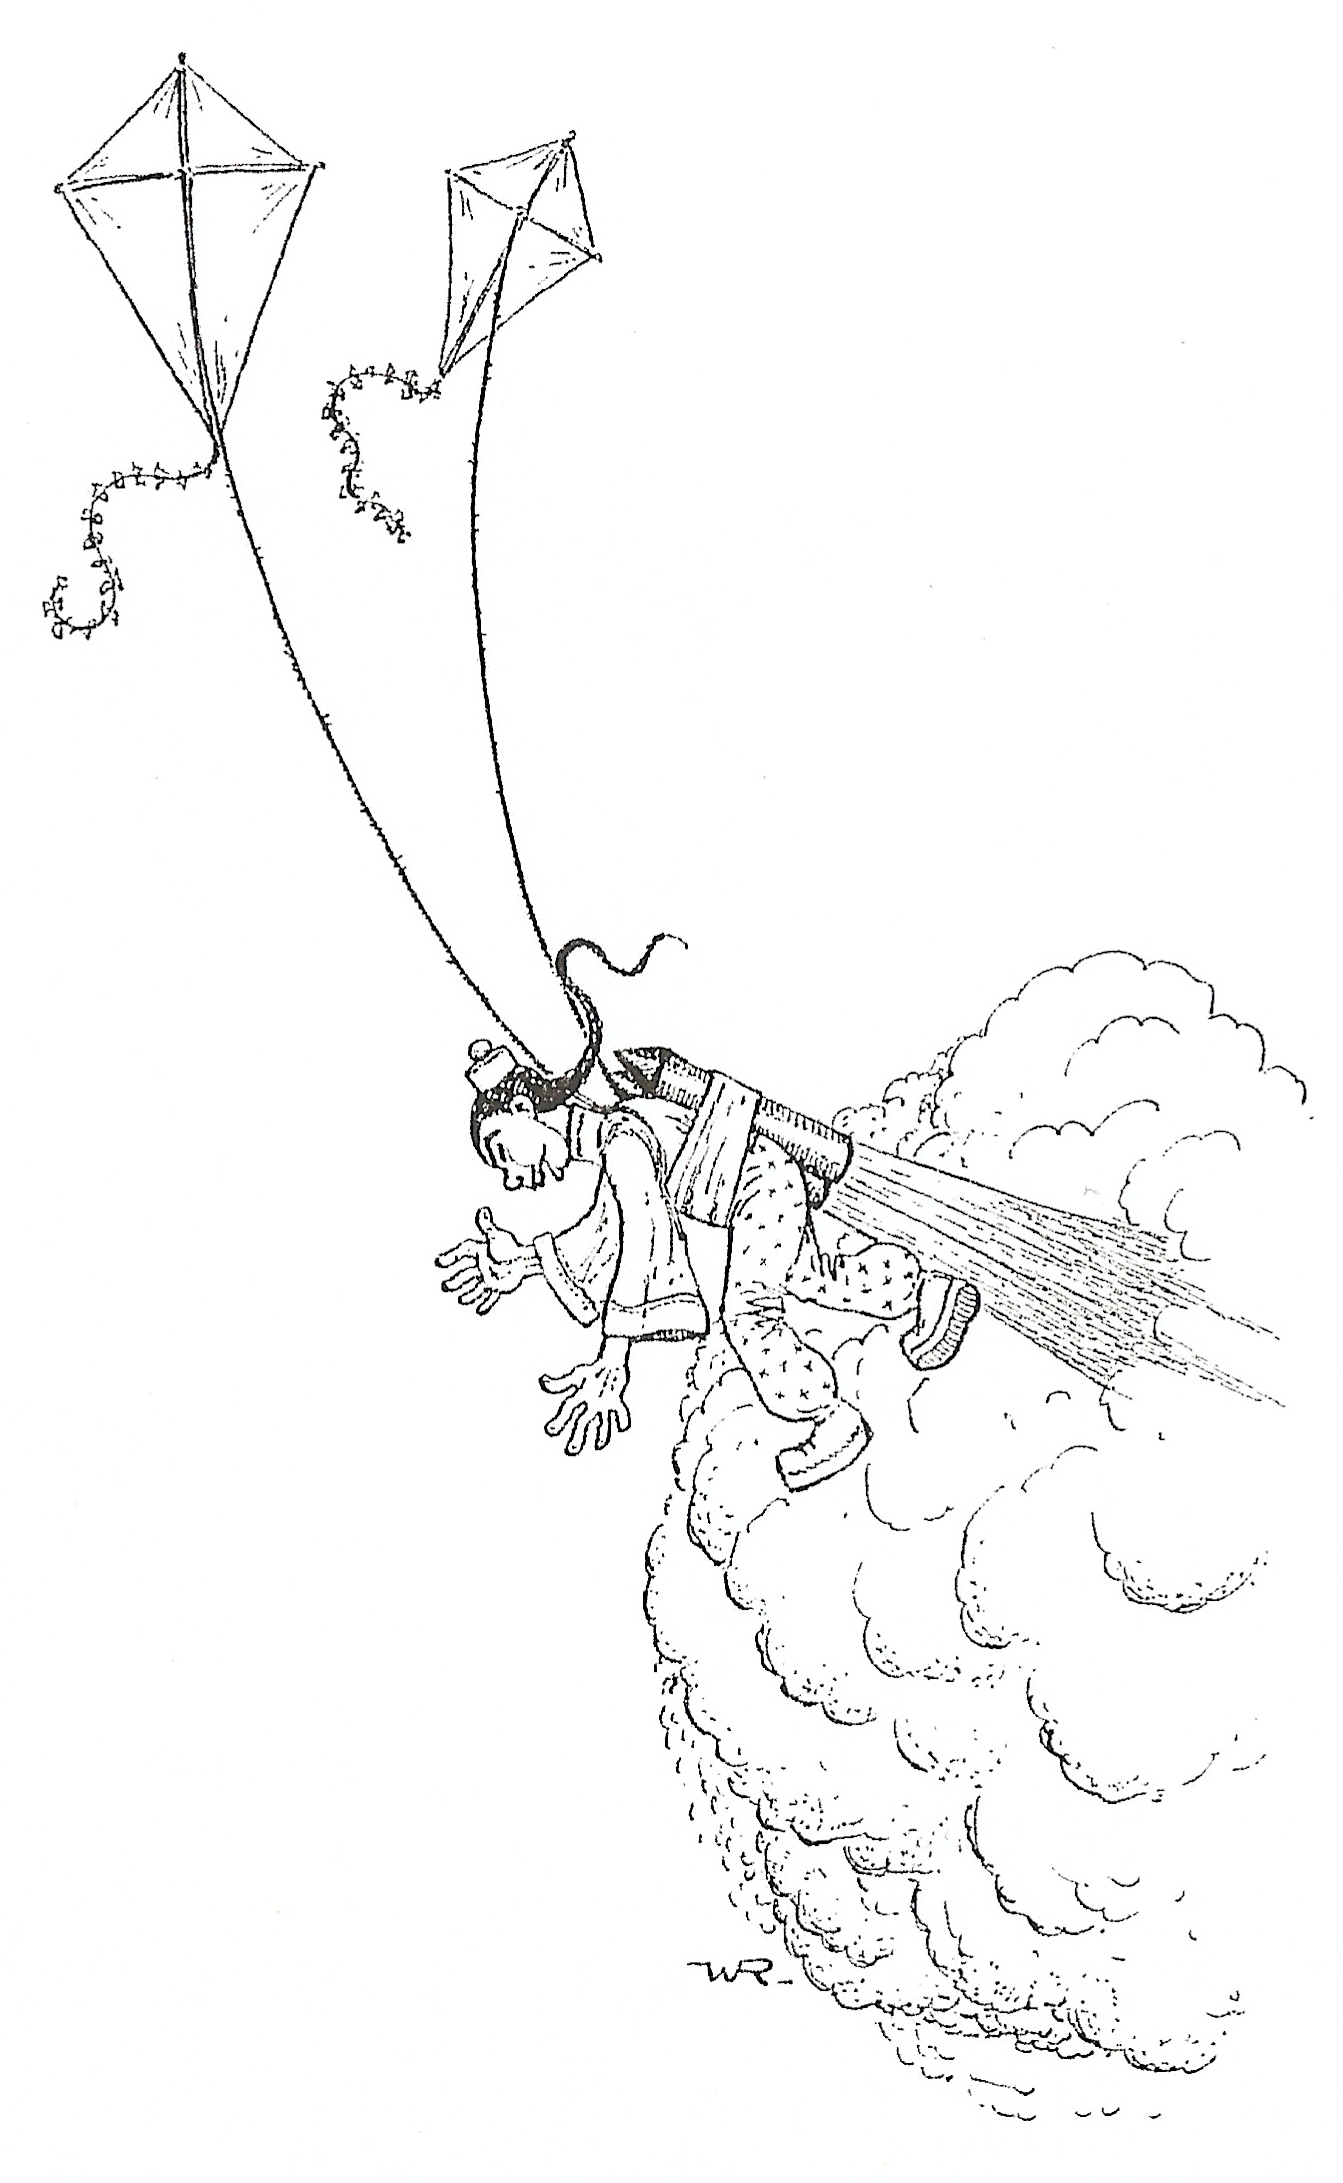
\includegraphics[width=90mm]{raket_dynamica}}
%%\put(45,100){\textsc{DEEL II}}
%\end{picture}
%\end{center}

\vfill

%\clearpage
%\newpage
%\thispagestyle{empty}
%\null
%\newpage


%!TEX root = ../cursus_fys6.tex

\chapter{De beginselen van Newton}
\label{debeginselenvannewton}

Het onderdeel binnen de mechanica dat zich met het verklarende principe bezighoudt, is de dynamica. Tot nu toe hebben we in de kinematica enkel bewegingen beschreven. We willen die bewegingen nu ook fysisch verklaren. De drie beginselen van Newton vormen, samen met enkele krachten, de fundamenten waarop de klassieke mechanica is gebouwd. 

\newpage

\section{De wet van de traagheid}

Op 22 oktober 1895 gebeurde er in het eindstation Gare Montparnasse -- Parijs, een ongeluk. De treinbestuurder was door het station gereden en pas 30 meter voorbij het einde van het spoor tot stilstand gekomen.
\begin{figure}[h]
\begin{center}
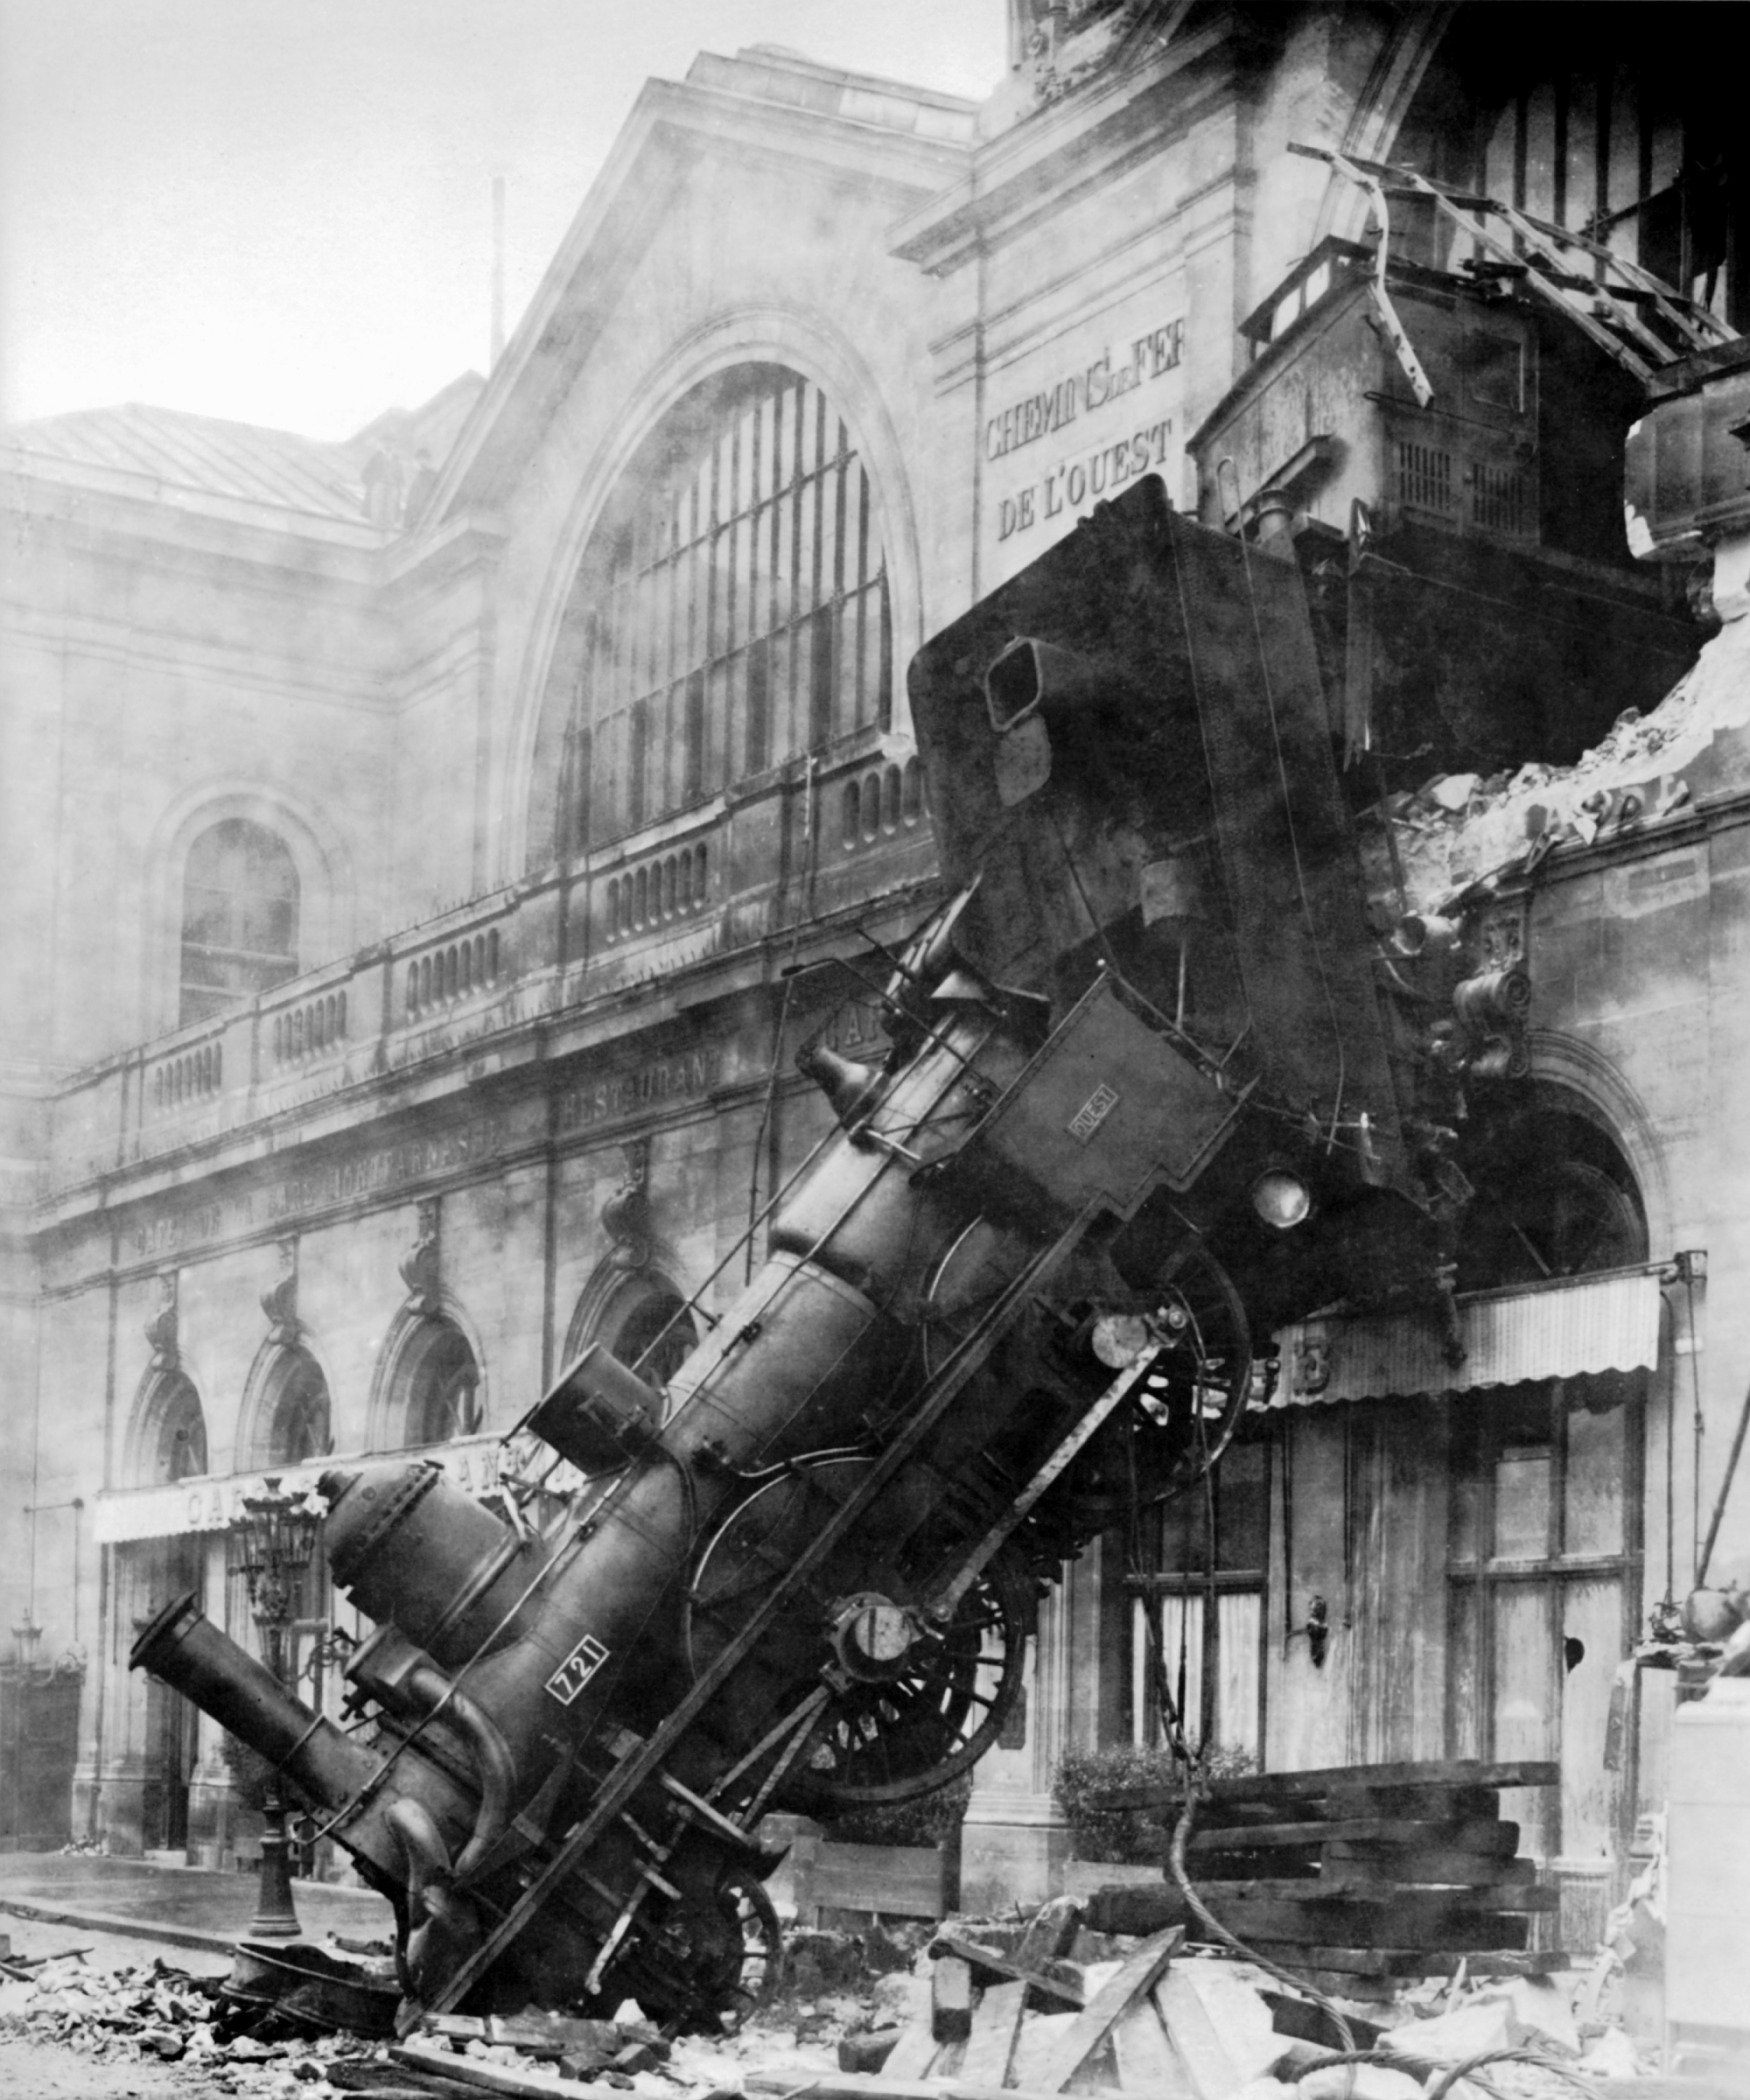
\includegraphics[width=.8\textwidth]{Train_wreck_at_Montparnasse_1895}
\caption{Gare Montparnasse. Parijs 1895}
\end{center}
\end{figure}

De figuur ademt de onvermijdelijke wet van de traagheid uit \ldots
\newline
\kader{
\vspace{1mm}
{\textbf{De wet van de traagheid}}

Een voorwerp behoudt zijn toestand van rust of van eenparige rechtlijnige beweging, tenzij er een resulterende kracht op werkt.
\vspace{3mm}}

Je zal zeggen dat je met die wet al vertrouwd bent. Maar zoals zo vaak, blijken we zonder het te beseffen niet zomaar alle consequenties in rekening te brengen. Onze ervaring uit het dagelijks leven
wil wel eens roet in het eten strooien. Zo zijn we vertrouwd met het feit dat
fietsen toch enige inspanning en dus kracht vergt. Zeker als de wind tegen zit.
We zouden dus kunnen aannemen dat -- willen we bewegen -- we steeds een kracht nodig
hebben en willen we harder bewegen, we een grotere kracht nodig hebben. Die kracht zou dan moeten dienen om om het streven naar de `natuurlijke' toestand van rust, tegen te gaan en de snelheid te onderhouden. Wat denk je, is dit niet in strijd met de wet van de traagheid \ldots?!\footnote{Als je tegen een topsnelheid van $300\rm\,km/h$ in de Thalys richting Parijs zit, voel je de zetel dan harder tegen jou duwen dan dat ze dat doet wanneer je nog stilstaat in Brussel-Zuid \ldots?}

Laten we -- om deze misvatting te bestrijden -- een gedachte-experiment uitvoeren. We doen dus niks concreets -- enkel redeneren. Het is een gedachte-experiment van Galileo Galilei (1564-1642). Om het uit te voeren hebben we een speciale knikkerbaan nodig, eentje zonder wrijving.\footnote{Ik heb horen zeggen dat er lang geleden een klein winkeltje bestond dat dergelijke knikkerbanen verkocht. Doorheen de jaren is het adres echter verloren gegaan. Niemand weet meer waar het zich bevindt \ldots} Laten we ervan uitgaan dat we in het bezit zijn van zo'n uiterst zeldzame baan. Onderstaande figuur toont dan de situatie waarin we een knikker op een bepaalde hoogte aan de linkerkant loslaten. Omdat er geen wrijving is, zal -- omwille van behoud van energie -- de knikker op de andere helling tot eenzelfde hoogte rollen, daar momentaan stilvallen en vervolgens terugrollen.
\begin{figure}[h]
\centering
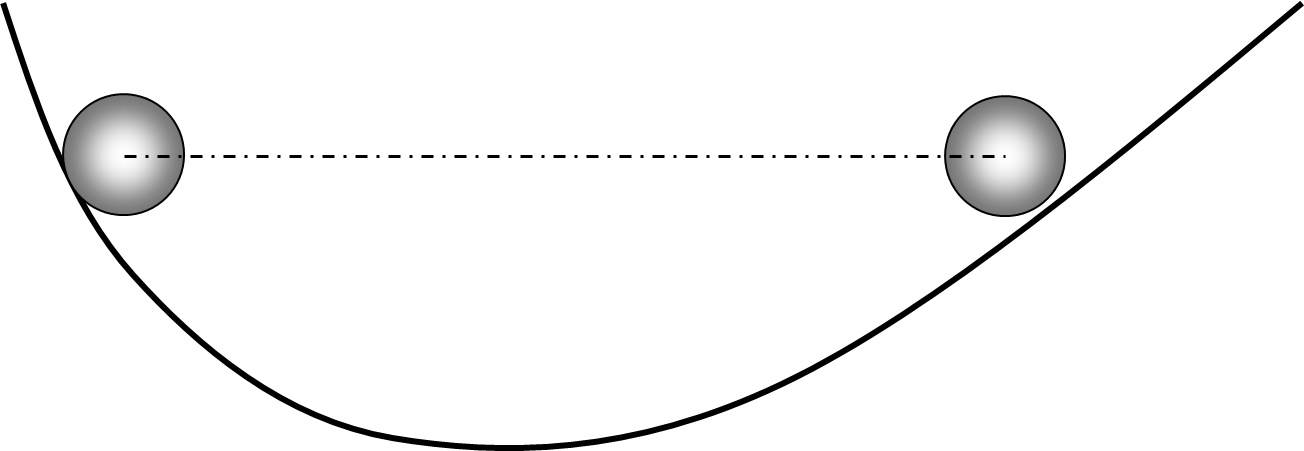
\includegraphics[width=.7\textwidth]{Afbeelding1}
%\caption{Het knikkertje rolt tot op dezelfde hoogte}
\label{Afbeelding1}
\end{figure}

Als we vervolgens de rechterhelling vlakker maken, zoals in onderstaande figuur, zal ons knikkertje ook nu tot dezelfde hoogte rollen. En dit ongeacht de grotere afstand. De energie-inhoud moet immers gelijk blijven.
\begin{figure}[h]
\centering
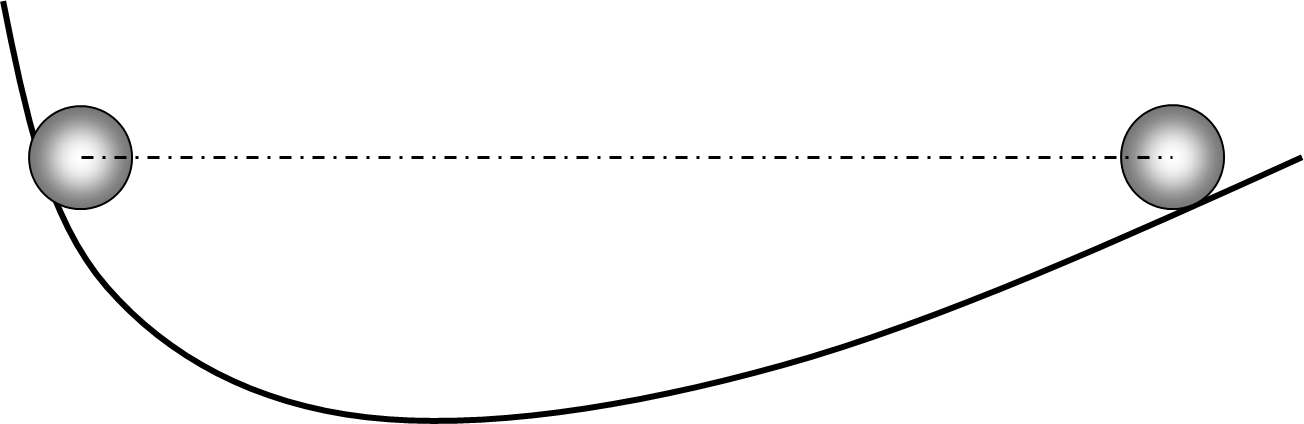
\includegraphics[width=.7\textwidth]{Afbeelding2}
\end{figure}

Als laatste stap in onze redenering, misleiden we ons knikkertje\footnote{Mag dat wel?}. Het knikkertje moet -- zo hebben we het hem verteld -- een tijdje horizontaal rollen om pas dan de rechterhelling te kunnen oprollen. Opnieuw tot dezelfde hoogte. Nu hebben we echter de rechterhelling oneindig ver weg gezet! Ons arm knikkertje zal dus blijven rollen (herinner u, er was geen wrijving) in de veronderstelling de helling ooit te zullen tegenkomen. 
\begin{figure}[h]
\centering
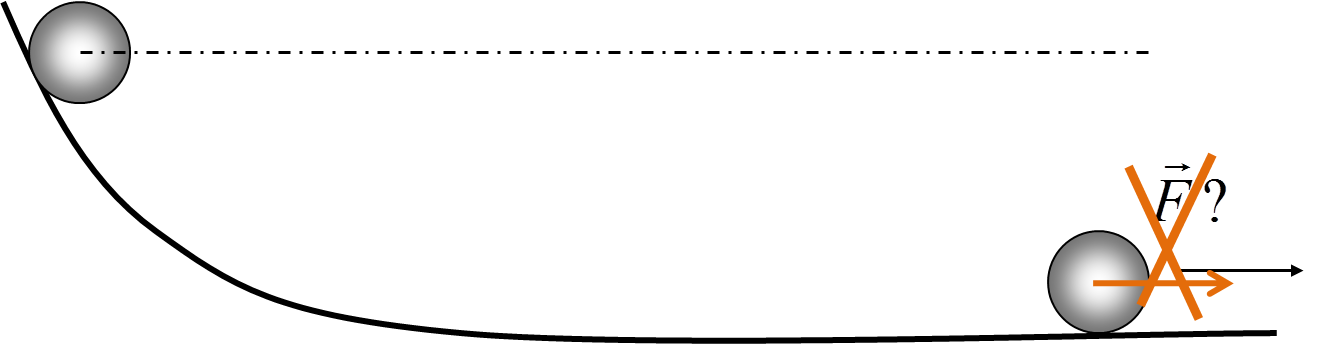
\includegraphics[width=.7\textwidth]{Afbeelding3}
\end{figure}
Gedurende het rollen op het horizontale stuk is de knikker dus niet onderhevig aan een voorwaartse kracht!\footnote{Wie zou immers die kracht uitoefenen \ldots?!} De beweging moet niet worden `onderhouden'. 

Uit ons gedachte-experiment kunnen we concluderen dat er een kracht nodig was om de knikker in beweging te brengen maar dat er \emph{geen} kracht nodig is om de beweging van de knikker op een rechte lijn en met een constante snelheid te onderhouden. Er is dus geen recht evenredig verband tussen kracht en snelheid \footnote{Moest je dat al denken.}. Kracht en snelheid kunnen zelfs tegengesteld zijn -- denk maar aan de wrijvingskracht die de beweging tegenwerkt.

De tendens van lichamen om zich te verzetten tegen de verandering van beweging, noemen we \textit{inertie} of \textit{traagheid}. Hoe groter de massa, hoe meer een voorwerp zich verzet.

\begin{figure}[h]
\centering

\includegraphics[width=0.8\textwidth]{Garfield_firstlaw}
\end{figure}

\voorbeeld{}{\textsf{
Wanneer je met de fiets fietst, rechtdoor en met een constante snelheid, is de kracht die je voorwaarts uitoefent dan groter, kleiner of gelijk aan de weerstandskracht die achterwaarts is gericht? Is met andere woorden de resulterende kracht op jouw fiets naar voren gericht, nul of naar achteren gericht? 
\newline
\newline Het antwoord is dat de resulterende kracht is nul is! Moest er immers een resulterende kracht zijn, dan zou volgens de wet van de traagheid de toestand van eenparige rechtlijnige beweging niet kunnen worden behouden. 
Eenmaal in beweging, is er geen kracht meer nodig om de beweging te onderhouden. Je moet blijven trappen om een even grote kracht als de weerstandskracht te kunnen genereren. Natuurlijk, om in beweging te komen, heb je wel een netto kracht naar voor toe nodig. Bij het remmen is de resulterende kracht dan weer naar achteren gericht.
}}

%\vfill


%\newpage

\section{Het tweede beginsel van Newton}

De eerste wet vertelt ons niet volledig wat er gebeurt wanneer op een lichaam een kracht werkt. Ze vertelt ons niet wat de relatie tussen kracht en beweging is. Uit onze dagelijkse ervaring zou je kunnen concluderen dat de snelheid van een voorwerp recht evenredig is met de erop uitgeoefende kracht. Hoe harder je immers op de pedalen duwt, hoe harder je gaat. De eerste wet vertelde ons echter al dat dit niet opgaat. 

Wat is dan de relatie tussen kracht en beweging? Een bal waar je harder tegen schopt, krijgt een grotere snelheid mee en een pingpongballetje vliegt gemakkelijker weg dan een basketbal of bowlingbal wanneer je er een tik tegen geeft. Als je het nader onderzoekt, door bijvoorbeeld verschillende krachten op een wagentje met eventueel steeds andere massa's te laten inwerken en de bijbehorende versnellingen te meten, merk je dat de versnelling recht evenredig is met de resulterende kracht en dat massa en versnelling omgekeerd evenredig zijn. M.a.w.
\begin{eqnarray*}
a\sim\frac{F}{m}
\end{eqnarray*}
%\begin{eqnarray*}
%\left.
%\begin{array}{l}
%\displaystyle
%a\sim F\\
%\displaystyle
%a\sim\frac{1}{m}
%\end{array}\right\}
%\Rightarrow a\sim\frac{F}{m}
%\end{eqnarray*}
Aangezien we met het fundament van de mechanica te maken hebben, kunnen we de eenheid van kracht zodanig kiezen dat de evenredigheidsconstante simpelweg 1 is. We defini\"eren dus \'e\'en newton als de kracht die een massa van \'e\'en kilogram een versnelling van \'e\'en meter per seconde kwadraat geeft. Samen met de observatie dat de versnelling dezelfde richting en zin als de kracht heeft, krijgen we de tweede wet van Newton.
\newline
\kader{
\vspace{3mm}
{\textbf{De tweede wet van Newton}}
\newline
\newline
De versnelling van een voorwerp is recht evenredig met de erop inwerkende resulterende kracht en omgekeerd evenredig met de massa van het voorwerp.
\begin{eqnarray*}
\vec{F}=m\vec{a}
\end{eqnarray*}
\vspace{0mm}}

Dit is misschien een gemakkelijke formule maar in al haar eenvoud \emph{immens} krachtig. Het is een wetmatigheid die een relatie geeft tussen de oorzaak (de krachten) en het gevolg (de beweging, strikt genomen de versnelling). Deze wetmatigheid is het verklarende principe achter alle mechanische bewegingen. Als we de krachten kennen, kennen we de versnelling van het voorwerp en kunnen we (althans op zijn minst in theorie) de baan van het voorwerp bepalen.


\section{Het derde beginsel van Newton}

Meestal plooien we onze vingers naar onze handpalm toe. De praktijk leert ons dat het andersom toch iets moeilijker gaat. Misschien vandaar. Als je echter met je andere hand wat helpt en duwt -- een kracht uitoefent -- plooien je vingers al iets verder naar achter. Uit zichzelf geraken ze niet zo ver. Als je nu -- ter vergelijking -- met gestrekte vingers tegen de tafel duwt, plooien je vingers eveneens meer naar achteren dan dat ze uit zichzelf zouden kunnen. Je moet concluderen dat naast het feit dat je een kracht op de tafel uitoefent\footnote{Misschien nu met weinig beweging tot gevolg.} de tafel op zijn beurt een kracht op je vingers uitoefent. Zonder extern inwerkende kracht zouden je vingers immers niet zo ver kunnen doorbuigen.
%\begin{figure}[h]
%\begin{center}
%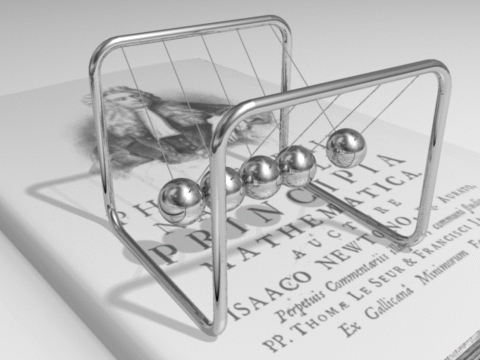
\includegraphics[width=.45\textwidth]{Newtons_cradle_animation_book}
%\caption{Een fascinerend speeltje}
%\end{center}
%\end{figure}
\begin{wrapfigure}{R}{0.5\textwidth}
\centering
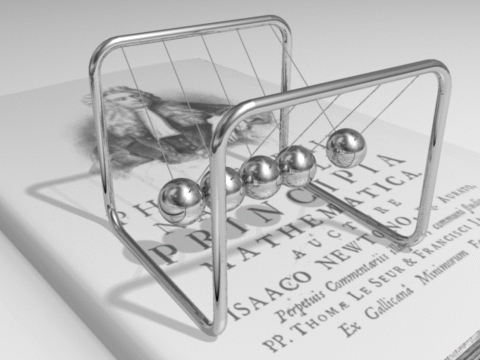
\includegraphics[width=0.44\textwidth]{Newtons_cradle_animation_book}
\caption{Een fascinerend speeltje}
\end{wrapfigure}
Een ander voorbeeld waarin lichamen krachten op mekaar uitoefenen is zo'n decoratief speeltje waar opgehangen metalen bolletjes op een fascinerende manier al botsend heen en weer slingeren. Een bolletje dat met een snelheid aangeslingerd komt, wordt tot stilstand gebracht terwijl een ander bolletje vanuit stilstand tot dezelfde snelheid wordt gelanceerd. Omdat de massa's van de kogeltjes even groot zijn en de versnelling van de ene even groot is als de vertraging van de andere, moeten de kogeltjes op elkaar even grote krachten uitoefenen. De derde wet van Newton -- ook wel de wet van actie en reactie genoemd -- \textit{poneert} dat de krachten die lichamen wederzijds uitoefenen \textit{altijd} even groot zijn.
\newline
\kader{
\vspace{1mm}
{\textbf{De wet van actie en reactie}}
\newline
\newline
Wanneer lichaam A op lichaam B een kracht uitoefent, oefent lichaam B op lichaam A een even grote maar tegengestelde kracht uit.
\begin{eqnarray*}
\vec{F}_{a,b}=-\vec{F}_{b,a}
\end{eqnarray*}
\vspace{0mm}
}

Met deze derde wet kunnen we verschillende verschijnselen verklaren. Zo is de wet van actie en reactie van toepassing op wandelen. Wij kunnen vanuit rust in beweging komen door ons af te zetten. Wij oefenen een kracht op de grond uit waarbij deze laatste op zijn beurt een even grote en tegengestelde kracht op ons uitoefent. Zo krijgen wij een versnelling. Een vliegtuig met straalmotoren of een raket doen hetzelfde. Door het uitoefenen van een kracht op de naar achter uitgeworpen gassen, oefenen de uitgeworpen gassen een kracht uit op het vliegtuig of de raket. Maar dan voorwaarts. (Een vliegtuig of raket duwt zich dus niet af tegen de (eventuele) lucht.)

Het even groot zijn van die krachten is misschien opmerkelijk. Het is toch de appel die naar de aarde valt en niet andersom?! Of, als de kracht die de aarde op de appel uitoefent even groot is als die de appel op de aarde uitoefent, waarom gaan ze dan niet naar mekaar toe? Het antwoord is dat de \emph{uitwerking} van een kracht niet hetzelfde is als de kracht zelf. De massa van de aarde is gigantisch veel groter dan die van de appel zodat die, volgens de tweede wet van Newton, een veel kleinere versnelling krijgt. En het is de versnelling die we zien, niet de kracht.

\newpage

\section{Oplossingsstrategie}

Bij het oplossen van vraagstukken waarin de wetten van Newton worden gebruikt, kan een vast stramien of heuristiek gebruikt worden. Omdat elke opgave anders is, blijft creativiteit noodzakelijk.
\begin{enumerate}
\item Bepaal het systeem dat je wilt beschouwen. Kies een systeem (object, lichaam, massa, geheel van lichamen) waarvan je een onbekende kracht of versnelling wilt berekenen. Kies een samengesteld systeem als je hierover informatie hebt.
\item Maak het systeem vrij. Beschouw het systeem als een vrij lichaam waarop alle uitwendige krachten inwerken. Teken al deze krachten die op het systeem werken. Dus niet de krachten die het systeem op zijn omgeving uitoefent. Die grijpen immers aan op een ander object. Het systeem waarop alle uitwendige krachten zijn getekend, wordt ook wel een krachtendiagram genoemd.
\item Pas de tweede wet van Newton toe op het systeem. Dit betekent dat de som van alle uitwendige krachten gelijk is aan de massa van het beschouwde systeem vermenigvuldigd met zijn versnelling:
\begin{eqnarray*}
\sum_{i=1}^n\vec{F}_i=m\vec{a}
\end{eqnarray*}
\item Kies een referentiestelsel en projecteer de vectorvergelijking. Ontbind de vectorvergelijking a.h.v. de eenheidsvectoren volgens de assen van een goed gekozen referentiestelsel. Op die manier bekom je
twee vergelijkingen die equivalent zijn met de vectorvergelijking:
\begin{eqnarray*}
x-as&:&\sum_{i=1}^nF_{i,x}=ma_x\\
y-as&:&\sum_{i=1}^nF_{i,y}=ma_y
\end{eqnarray*}
Hierin zijn $F_{i,x}$ en $F_{i,y}$ de componenten van de verschillende krachten volgens respectievelijk de $x$-as en de $y$-as.
\item Kies een tweede, derde \ldots systeem en herhaal stap 1 t/m 4. Indien er meer dan \'e\'en onbekende is, moet je nog andere systemen beschouwen. Kies ze zodanig dat je de derde wet van Newton kunt gebruiken tussen de verschillende systemen of dat de versnelling dezelfde is.
\item Los het stelsel vergelijkingen op.
\end{enumerate}

\newpage

\voorbeeld{}{\textsf{
\begin{enumerate}
\item[Opgave] Twee massa's $m_1$ en $m_2$ zijn via een touwtje en een katrol van te verwaarlozen massa met elkaar verbonden zoals in de figuur. Er is geen wrijving aanwezig. De massa's hebben een versnelling zoals aangegeven.
\newline
Bepaal de grootte van de versnelling van beide massa's en de grootte van de spankracht in het touw.
\begin{figure}[h]
\begin{center}
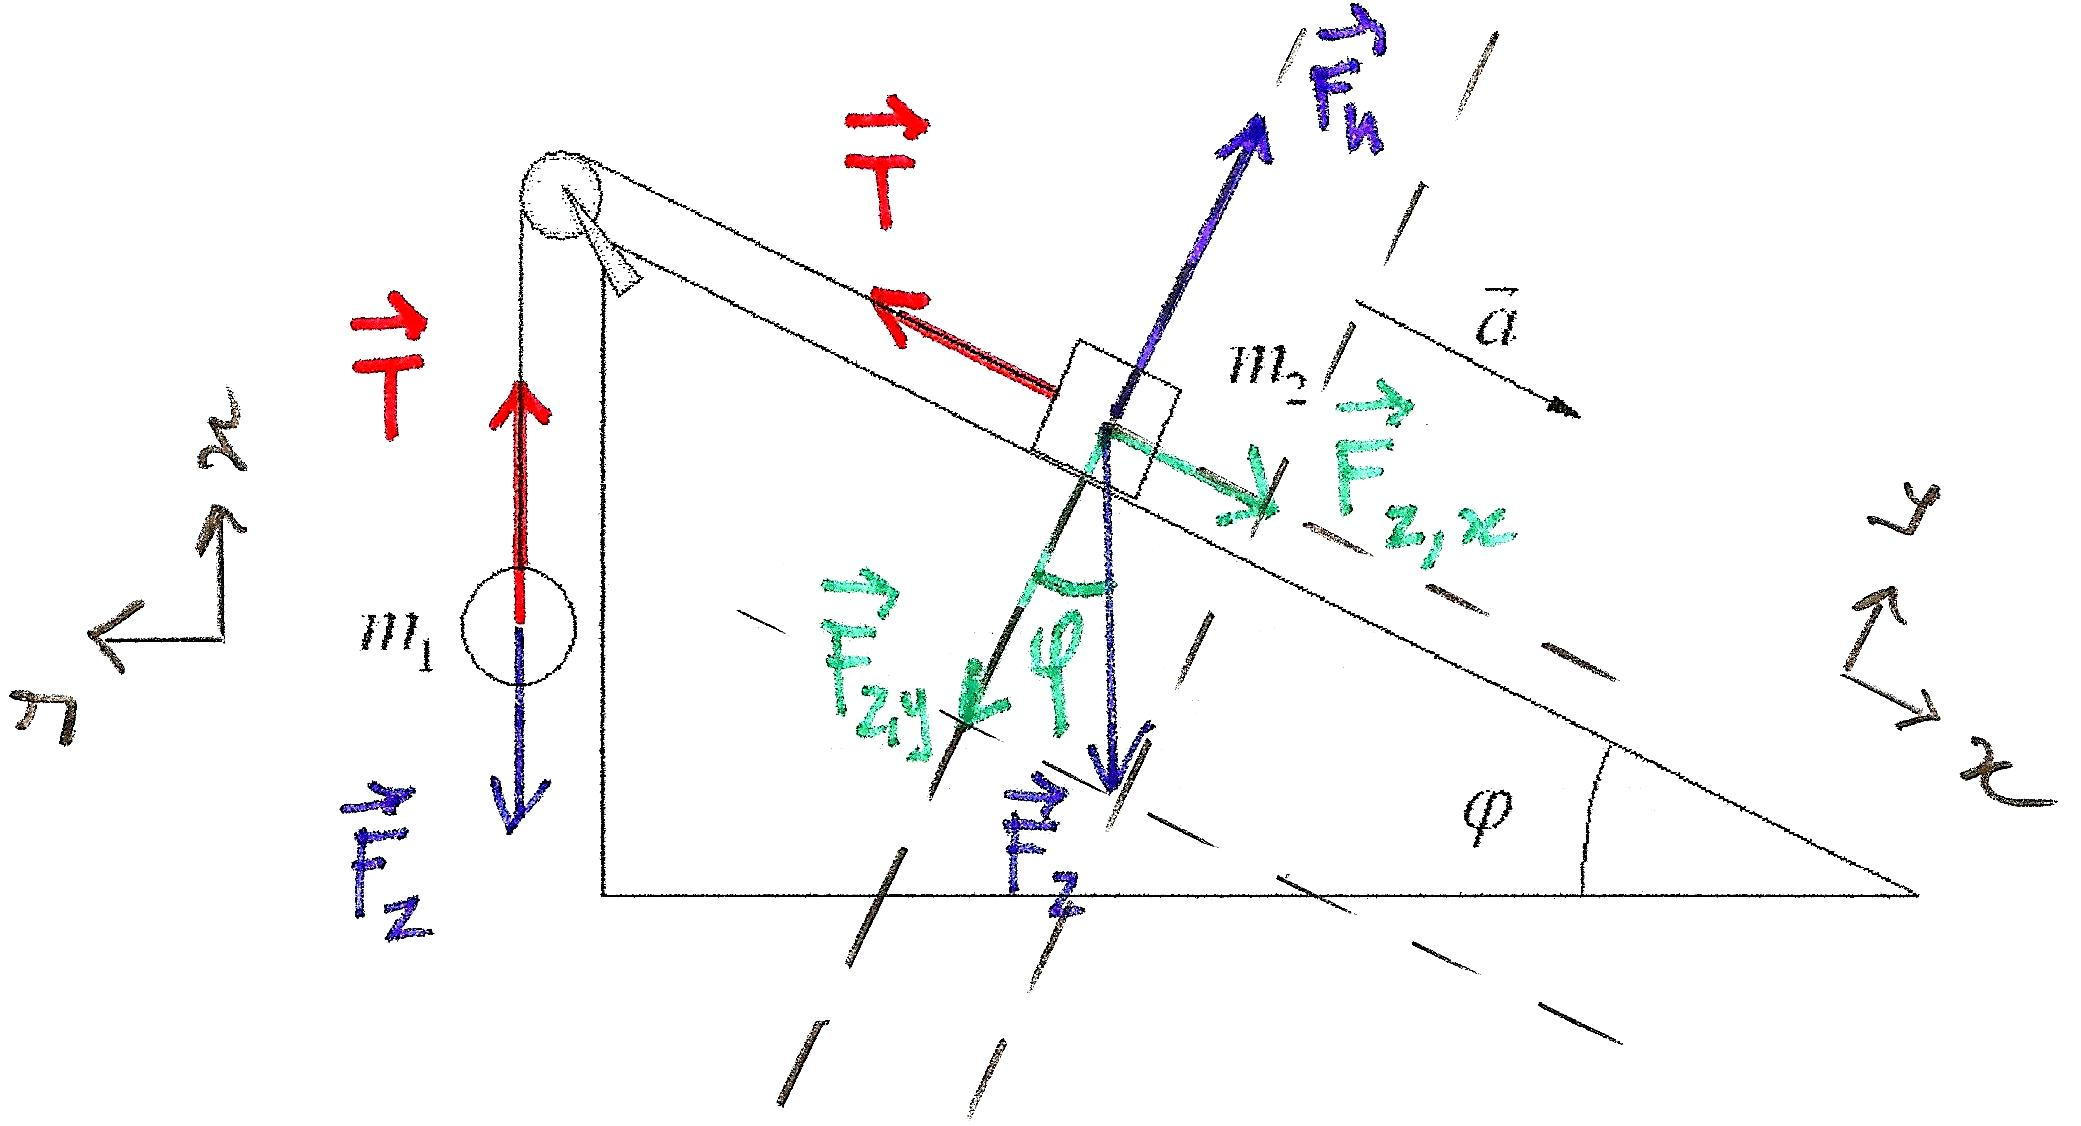
\includegraphics[width=0.45\textwidth, angle=0]{blokken_helling_opl}
\end{center}
\end{figure}
\item[gegeven]$m_1,~m_2,~\varphi$
\item [gevraagd]$a$, $F_s$
\item [oplossing]De tweede wet van Newton toepassen op $m_1$ levert
\begin{eqnarray}
F_s-m_1g&=&m_1a\nonumber\\
&\Updownarrow&\nonumber\\
F_s&=&m_1(a+g)\label{T1}
\end{eqnarray}
De tweede wet van Newton toepassen op $m_2$, met $F_z=mg$, levert
\begin{eqnarray}
F_{z,x}-F_s&=&m_2a\nonumber\\
&\Updownarrow&\nonumber\\
F_s&=&m_2(g\sin{\varphi}-a)\label{T2}
\end{eqnarray}
Uit (\ref{T1}) en (\ref{T2}) volgt
\begin{eqnarray}
%m_1(a+g)&=&m_2(g\sin{\varphi}-a)\nonumber\\
%&\Updownarrow&\nonumber\\
a&=&\frac{m_2\sin{\varphi}-m_1}{m_1+m_2}g\nonumber
\end{eqnarray}
Dit resultaat substitueren in (\ref{T2}) levert, na het uitwerken door op ge\-lij\-ke noemer te zetten:
\begin{eqnarray}
F_s&=&\frac{m_1m_2g(1+\sin{\varphi})}{m_1+m_2}\nonumber
\end{eqnarray}
\end{enumerate}
}}


\newpage


\section*{Dialogo sopra i due massimi sistemi del mondo}

Galileo schreef in 1632 een dialoog waarin hij de juistheid van het copernicaanse wereldbeeld fysisch probeerde te bewijzen door middel van de socratische methode\footnote{Van Dale: waarbij men de denkbeelden uit de geest van de leerling zelf ontwikkelt, terwijl men hem door gepaste vragen allengs zo ver brengt, dat hij het begrip, dat men hem duidelijk wil maken, zelf vindt.}. Een van de tegenargumenten was dat een vallende steen niet volgens een loodlijn op het aardoppervlak zou neerkomen, wanneer de aarde zelf een rotatie uitvoerde.\footnote{De aarde zou immers onder de steen wegdraaien.} Galileo haalde dit argument onderuit door gebruik te maken van het traagheidsbeginsel (anderen hadden dit ook geprobeerd via een 'slepende invloed' van de lucht, maar Galileo zag in dat dat niet voldoende was en erkent de ware fysische grondslag).
De dialoog gaat tussen drie geleerden. Sagredo is de vriend van een niet nader genoemd auteur (Galileo), die zijn gesprekspartners inlicht over diens nieuwe theori\"en. Salviati is de onbevooroordeelde geleerde die vooral zijn gezond verstand gebruikt, en dus de positie van de lezer verbeeldt. Simplicio is de wat simplistische schoolgeleerde (scholasticus), die het standpunt van Aristoteles weergeeft.
%\newline
%\newline
Hier een fragment uit deze dialoog.

\vfill

{\footnotesize

\begin{enumerate}
\item[SALVIATI]U zegt: aangezien bij een stilliggend schip een [vallende] steen aan de voet van de mast neerkomt, bij een bewegend schip daarentegen op enige afstand van de voet, kan men daaruit omgekeerd besluiten dat wanneer de steen aan de voet neervalt, het schip in rust is; en ook, dat wanneer het op enige afstand neerkomt, dat het schip dan beweegt. Aangezien datgene wat voor een schip geldt ook voor de hele Aarde moet gelden, volgt hieruit dat uit het neervallen van de steen aan de voet van de toren noodzakelijk tot de onbeweeglijkheid van de Aarde mag besloten worden. Is dat niet uw bewijs?
\item[SIMPLICIO]Ja, en op een zeer beknopte manier weergegeven, wat erg bijdraagt tot het goede begrip ervan.
\item[SALVIATI]Zeg me nu: als een uit de top van de mast losgelaten steen ook bij een snel bewegend schip precies op die plaats neervalt, waar het ook bij een stilliggend schip zou neerkomen, welke waarde zouden dan deze valexperimenten hebben voor het bepalen van de beweging of rust van het schip?
\item[SIMPLICIO]Helemaal geen waarde. Net zoals men uit de hartslag niet kan besluiten of iemand slaapt of wakker is, aangezien de hartslag op gelijke wijze klopt bij slapenden of wakenden.
\item[SALVIATI]Zeer goed. Hebt u ooit het experiment met het schip uitgevoerd?
\item[SIMPLICIO]Dat heb ik niet gedaan, maar ik denk wel dat de auteurs die ik daarnet genoemd heb, het zeer zorgvuldig hebben gecontroleerd. Bovendien ligt de oorzaak van het onderscheid zo voor de hand, dat hier nauwelijks enige ruimte voor twijfel overblijft.
\item[SALVIATI]Dat bepaalde auteurs het experiment mogelijk vermelden, zonder het zelf te hebben uitgevoerd, daarvan bent u zelf het beste bewijs. Want zonder het experiment te hebben uitgevoerd, noemt u het zeker en vertrouwt u op het woord van anderen. Net zo hebben mogelijk -- nee wel zeker -- ook die auteurs gehandeld, namelijk zich op hun voorgangers beroepen, zonder dat men ooit op een getuigenis is gestoten van iemand die het experiment werkelijk had uitgevoerd. Want iedereen die het uitvoert, zal vinden dat precies het tegenovergestelde plaatsvindt van datgene wat men in de boeken leest. Men zal namelijk tot het inzicht komen, dat de steen steeds op dezelfde plaats van het schip neervalt, of dat nu in rust is of in beweging met een willekeurige snelheid. En vermits de Aarde en het schip dezelfde verschijnselen moeten vertonen, zo mag men uit de loodrechte val van de steen en de inslag aan de voet van de toren niets besluiten over de beweging of de rust van de Aarde.
\item[SIMPLICIO]Als u mij niet het experiment als leidraad had aangewezen, dan zou onze discussie nog niet zo snel afgelopen zijn. Want dit probleem lijkt mij voor de menselijke rede zo moeilijk toegankelijk dat niemand hierin met enige geloofwaardigheid licht kan zien. 
\item[SALVIATI]En toch wil ik precies dat beweren.
\item[SIMPLICIO]U heeft dus niet eens honderd, zelfs niet \'e\'en experiment uitgevoerd en toch bent u reeds zeker van het resultaat? Ik hou vast aan mijn ongeloof en mijn aanvankelijke overtuiging, namelijk dat de voornaamste auteurs die het experiment vermelden, het ook uitgevoerd hebben en met de door hen aangegeven resultaten.
\item[SALVIATI]Ik ben zonder experiment zeker dat het experiment z\'o zal gebeuren zoals ik zeg, want het kan niet anders. Ja, meer nog, ik beweer zelfs dat u ook weet dat het resultaat niet anders kan zijn, al meent u of doet u zich voor het niet te weten. Ik versta echter de techniek om met hersens om te gaan zo meesterlijk, dat ik u zelfs tegen uw zin zal doen bekennen. [ ... ]
\item[SIMPLICIO]Ik zal uw vragen beantwoorden naar best vermogen, want ik ben zeker dat ik niet in moeilijkheden zal komen. Want van dingen waarvan ik weet dat ze niet waar zijn, kan ik toch moeilijk enige kennis hebben, aangezien kennis enkel kan bestaan over ware en niet over onware dingen.
\item[SALVIATI]Ik wil niet dat u mij iets antwoordt waarvan u niet zeker bent. Zeg me dan: als u een vlak oppervlak neemt, zo glad als een spiegel en gemaakt van een hard materiaal zoals staal, dat niet horizontaal is, maar een beetje hellend, en u legt daarop een perfect ronde kogel uit een zware, zeer harde stof, bijvoorbeeld brons, wat zal volgens u deze kogel, volledig aan zichzelf overgelaten, doen ? Meent u niet, net als ik, dat hij gewoon ter plaatse zal blijven liggen?
\item[SIMPLICIO]En het vlak is hellend?
\item[SALVIATI]Inderdaad, die onderstelling heb ik gemaakt. 
\item[SIMPLICIO]Ik geloof helemaal niet dat hij blijft liggen; in tegendeel, ik ben heel zeker dat hij uit zichzelf naar beneden zal rollen.
\item[SALVIATI]Let wel wat u zegt, Signor Simplicio; ik ben er namelijk van overtuigd dat de kogel overal zal blijven liggen, waar u hem ook legt.
\item[SIMPLICIO]Als u zich op zulke opvattingen vertrouwt, dan sta ik er niet meer versteld van dat u tot valse resultaten komt.
\item[SALVIATI]U houdt het dus voor zeker dat de kogel vanzelf naar beneden zal rollen?
\item[SIMPLICIO]Wat een vraag!
\item[SALVIATI]En u betrouwt hierop, niet omdat ik het u geleerd zou hebben -- ik heb immers getracht u het tegendeel te laten beweren -- maar helemaal uit uzelf, door toedoen van gezond verstand?
\item[SIMPLICIO]Nu begrijp ik uw truukje; u hebt slechts zo gepraat om mij uit mijn schelp te lokken, zoals men zegt, niet omdat u zelf daar zo over dacht.
\item[SALVIATI]Inderdaad. Hoe lang en met welke snelheid zal nu die kogel naar beneden rollen? Let op dat ik het hier heb om een volkomen ronde kogel en een perfect glad oppervlak, zodat alle uitwendige en toevallige hindernissen worden uitgesloten. Zelfs vraag ik u ook abstractie te maken van de luchtweerstand en van alle andere weerstanden, voor zover die zouden aanwezig zijn.
\item[SIMPLICIO]Ik heb alles goed verstaan. Op uw vraag antwoord ik: de kogel zal oneindig lang blijven rollen, zo lang het hellend vlak doorloopt, en wel in een eenparig versnelde beweging. Want zoals de natuur van zware lichamen het voorschrijft: vires acquirunt eundo. Daarbij zal de snelheid des te groter zijn, naarmate de helling van het vlak groter is.
\item[SALVIATI]Als men nu echter wil dat de kogel op het zelfde vlak naar boven beweegt, zal hij dat in de werkelijkheid ook doen?
\item[SIMPLICIO]Niet uit zichzelf; wel als men hem met geweld naar boven schuift of stoot.
\item[SALVIATI]En als de kogel nu met een zekere impuls naar boven wordt gestoten, wat zal dan zijn beweging zijn?
\item[SIMPLICIO]De beweging zou steeds langzamer worden, omdat zij tegennatuurlijk is. Verder zal zij langer of korter duren afhankelijk van de kracht van de stoot of de grootte van de helling.
\item[SALVIATI]U hebt nu, zo lijkt mij, het gedrag van een bewegend lichaam op twee verschillende vlakken geschetst. Op het hellend vlak, zegt u, beweegt het zware lichaam zich spontaan naar beneden met een eenparig versnelde beweging en om hem daar in rust te houden, moet men een kracht aanwenden; bij een stijgende helling is daarentegen een kracht nodig om hem vooruit te drijven en ook om hem vast te houden. De meegegeven hoeveelheid beweging, zegt u verder, vermindert in dit geval voortdurend en verdwijnt tenslotte geheel. Verder stelt u nog dat in beide gevallen de helling van het vlak van belang is; namelijk dat enerzijds een grotere helling ook een grotere snelheid met zich mee brengt en anderzijds een bewegend lichaam op een stijgende helling des te langer blijft bewegen naarmate de helling minder steil is. Zeg me nu wat met het lichaam zou gebeuren op een horizontaal oppervlak, dat niet daalt en niet stijgt.
\item[SIMPLICIO]Hier moet ik toch even over het antwoord nadenken. Aangezien er geen neerwaartse helling is, is er ook geen natuurlijke neiging tot bewegen; aangezien er verder ook geen opwaartse helling is, kan er ook geen weerstand tegen de beweging aanwezig zijn. Het lichaam moet dan onverschillig blijven tussen de neiging tot bewegen en de weerstand tegen die beweging. Het moet dan, volgens mij, van nature uit in rust blijven. - Maar hoe vergeetachtig ben ik toch! Nog niet zo lang geleden heeft Signor Sagredo me reeds uitgelegd dat dit precies het geval moet zijn.
\item[SALVIATI]Dat is ook mijn mening, in de onderstelling dat men de kogel rustig neerlegt. Als men hem echter met een impuls in een bepaalde richting wegstoot, wat zal dan gebeuren?
\item[SIMPLICIO]Het lichaam zal dan in die richting bewegen.
\item[SALVIATI]Maar welke beweging, een eenparig versnelde beweging, zoals in het geval van een neerwaartse helling, of een eenparig vertraagde, zoals bij de opwaartse helling?
\item[SIMPLICIO]Ik kan geen oorzaak voor een versnelling of een vertraging ontdekken, aangezien er geen neerwaartse of opwaartse helling is.
\item[SALVIATI]Goed. Als er echter geen oorzaak voor een vertraging is, dan zal er zeker geen oorzaak zijn om het lichaam geheel tot stilstand te brengen. Hoe ver zal het lichaam dan blijven bewegen?
\item[SIMPLICIO]Zolang de uitgebreidheid van het horizontale vlak het toelaat.
\item[SALVIATI]Als dit vlak onbegrensd zou zijn, dan zou de beweging van het lichaam evenzo onbegrensd zijn. Dus eeuwig?
\item[SIMPLICIO]Zo lijkt het me wel, tenminste als het lichaam van een bestendig materiaal is gemaakt.
\item[SALVIATI]Dat nemen we inderdaad aan, zoals we reeds gezegd hebben; alle toevallige en uitwendige hindernissen werden verwijderd en de vergankelijkheid van het voorwerp is ook zo'n toevallige hindernis. Zeg mij nu: wat is volgens u de reden waarom die kogel op een dalende helling spontaan, op een stijgende helling slechts dwangmatig beweegt?
\item[SIMPLICIO]De reden daarvan is dat de natuurlijke neiging van een zwaar lichaam erop gericht is zich naar het middelpunt van de aarde te bewegen, terwijl de opwaartse beweging naar de grenzen van het universum slechts met geweld kan plaats vinden. Het afhellend vlak maakt een nadering van het middelpunt mogelijk, het stijgende vlak echter de verwijdering.
\item[SALVIATI]Een vlak dat dus niet afhelt of stijgt, moet dus in al zijn delen even ver verwijderd zijn van het middelpunt. Bestaan dergelijke vlakken in de wereld?
\item[SIMPLICIO]Zo zijn er heel veel, bijvoorbeeld het aardoppervlak als het tenminste perfect glad zou zijn, en niet ruw en bergachtig, zoals het in werkelijkheid is. Maar neem bijvoorbeeld het wateroppervlak, zolang het water rustig en kalm is.
\item[SALVIATI]Een schip dat op een kalme zee vaart is dus zo een van de lichamen die zich voortbewegen op een horizontaal vlak, zoals we besproken hebben. Het zal dan ook, na wegnemen van alle toevallige en uitwendige hindernissen, voortdurend en onveranderd blijven voortbewegen met zijn eenmaal meegedeelde beginsnelheid.
\item[SIMPLICIO]Zo moet het zijn, lijkt me.
\item[SALVIATI]Nu, wat betreft de steen in de top van de mast. Beweegt die ook niet, gedragen door het schip, op een cirkelvormige baan rondom het middelpunt van de Aarde? Met andere woorden, heeft die steen geen beweging die, afgezien van uitwendige hindernissen, onuitwisbaar blijft voortbestaan? En is die beweging niet net zo snel als die van het schip?
\item[SIMPLICIO]Dat is allemaal juist. En dan?
\item[SALVIATI]Trek nu zelf het besluit uit het voorgaande, aangezien u alle premissen kent.
\item[SIMPLICIO]U bedoelt met het besluit, dat de steen, die beweegt met een onuitwisbare gedwongen beweging, deze beweging niet verliest [tijdens de val], maar het schip blijft volgen en tenslotte op dezelfde plek zal neerkomen als wanneer het schip stil ligt. En ik ook zeg dat dit het geval moet zijn als er geen uitwendige oorzaken zijn die de beweging van de losgelaten steen verstoren.
\end{enumerate}

}

\newpage

Het traagheidsbeginsel had bij Galilei nog geen universele status. Het ging slechts om een eigenschap van bewegingen van zware lichamen op een concentrische baan omheen het middelpunt van de aarde.
\newline
\newline
Hier een fragment uit Descartes' natuurkundeleerboek \textit{Principia Philoso\-phiae} (uitgegeven bij Elzevier te Leiden, 1644).
Descartes was een rationalist, d.w.z. dat hij de fundamentele natuurwetten baseerde op helder en `onbetwijfelbare' idee\"en in zijn geest, of bijvoorbeeld in de afwezigheid van redenen om iets anders aan te nemen. (`Waarom zou God ons misleiden door ons verkeerde idee\"en te laten denken?'). Descartes gaat iets verder dan Galilei, bij hem is het beginsel een algemene natuurwet, die niet enkel beperkt is tot zware voorwerpen onder invloed van de zwaartekracht, maar die inherent is aan het verschijnsel beweging.
\newline
\newline

{\footnotesize

\begin{enumerate}
\item[]\textit{De eerste wet der natuur: dat elk voorwerp blijft in die staat waarin het zich bevindt, zolang niets het verandert.}
Uit het feit dat ook God niet aan verandering onderhevig is, en dat Hij altijd op dezelfde wijze handelt, kunnen we kennis verwerven van bepaalde regels, die ik noem de wetten van de natuur, en die de oorzaken zijn van de verschillende bewegingen die we in alle lichamen waarnemen; belangrijk genoeg dus om hier te vermelden. De eerste is dat elk voorwerp voor zover mogelijk in dezelfde toestand blijft en die toestand slechts verandert door de interactie met andere. Zo zien we elke dag dat een vierkant voorwerp vierkant blijft, indien niets de vorm ervan wijzigt; en dat, als het voorwerp in rust is, het niet uit zichzelf begint te bewegen. Maar eenmaal het begonnen is te bewegen, hebben we ook geen enkele reden om te denken dat het ooit op eigen kracht zal ophouden te bewegen, zolang het niets ontmoet dat zijn beweging tegenhoudt of stopt. Zodat als een lichaam eenmaal begint te bewegen, wij moeten besluiten dat het steeds verder zal blijven bewegen, en dat het nooit uit zichzelf zal stoppen. Omdat we echter op een aarde leven die zodanig is opgebouwd dat alle bewegingen in onze omgeving vrij snel tot stilstand komen, en vaak door oorzaken die we met onze zintuigen niet kunnen waarnemen, oordelen we van jongs af aan dat de bewegingen die zo tot stilstand komen, dat uit zichzelf doen en hebben we nog steeds de neiging dat te geloven van alle bewegingen in de wereld, namelijk dat ze vanzelf tot stilstand komen en naar stilstand neigen, omdat we menen dat daarvan veelvuldige waarnemingen hebben gedaan. Nochtans is dat een verkeerd vooroordeel, dat duidelijk ingaat tegen de wetten van de natuur, want de rust is tegengesteld aan de beweging en niets zal door eigen instinct geneigd zijn tot zijn natuurlijk tegengestelde, of tot de vernietiging van zichzelf. [...]

\item[]\textit{De tweede wet van de natuur: dat elk bewegend lichaam zijn beweging zal trachten voort te
zetten volgens een rechte lijn.} De tweede wet die ik in de natuur opmerk, is dat elk deel van de materie op zich genomen nooit ernaar streeft zijn beweging verder te zetten volgens een gebogen baan, maar volgens een rechte lijn, hoewel vele lichamen kunnen gedwongen zijn af te buigen omdat ze andere lichamen op hun weg ontmoeten. [...] Deze wet, zoals de voorgaande, hangt af van het feit dat God onveranderlijk is, en dat hij de beweging van de materie behoudt door een eenvoudige handeling [namelijk van ogenblik tot ogenblik]. En hoewel de beweging zich niet voltrekt in een [ondeelbaar] ogenblik, toch is het duidelijk dat elk bewegend lichaam een richting aanhoudt volgens een rechte lijn en niet volgens een cirkelvormige. [...]

\item[]\textit{Waarin bestaat de kracht van een lichaam om te handelen of te weerstaan.} De kracht waarmee een lichaam inwerkt op een ander of de inwerking van dat andere lichaam weerstaat, ligt enkel hierin, dat elk ding voor zover mogelijk volhardt in de toestand waarin het zich bevindt, overeenkomstig de eerste wet. Zodat een lichaam dat verbonden is met een ander voorwerp een zekere kracht bezit om te verhinderen dat het ervan gescheiden wordt; en dat, wanneer het ervan gescheiden is, het een zekere kracht bezit om te verhinderen dat het ermee verbonden wordt. Ook, wanneer het in rust is, bezit het kracht om in rust te blijven en om te weerstaan aan alles wat het zou doen veranderen. Net als elk bewegend lichaam een kracht heeft om te blijven bewegen met dezelfde snelheid en in dezelfde richting. Men kan de grootte van deze kracht inschatten door de grootte van het voorwerp waarin ze huist, en van het oppervlak volgens hetwelk een voorwerp van een ander wordt gescheiden, en ook door de snelheid en de manier waarop botsende lichamen elkaar ontmoeten.

\end{enumerate}

}

De vruchtbaarheid van het traagheidsbeginsel komt pas goed tot uiting in het werk van Christiaan Huygens (1629-1695). Voor Huygens is het beginsel een algemeen aanvaard axioma waaruit de relativiteit van inerti\"ele stelsels kan afgeleid worden. Huygens ziet hierin een middel om de wetten van elastische botsing af te leiden, wat rond het midden van de zeventiende eeuw een nog helemaal onopgelost probleem
was. Descartes had met zijn traagheidsbeginsel een aantal botsingswetten geformuleerd die echter duidelijk fout waren, o.a. omdat de verschillende regels bij grensgevallen niet in elkaar overgingen. Huygens werkte op dit probleem vermoedelijk al in 1656, maar publiceerde pas in 1669 een kort verslag van zijn resultaten in de \textit{Philosophical Transactions} -- zonder enig bewijs. Pas na zijn dood werd het hele traktaat in zijn postuum \textit{Opuscula varia} (Leiden, 1703) openbaar gemaakt. Het geldt nog steeds als \'e\'en der mooiste teksten van de vroege fysica. De volgende tekst is de aanvang van het traktaat.
\newline
\newline
{\footnotesize

\begin{enumerate}
\item[Axioma 1] Een eenmaal bewogen lichaam zet, wanneer niets het belet, zijn beweging standvastig
voort met dezelfde snelheid en in rechte lijn.

\item[Axioma 2] Wat ook de oorzaak mag zijn van de botsing van twee harde lichamen, wij nemen de
volgende stelling aan: wanneer twee gelijke lichamen met gelijke snelheden uit tegenovergestelde
richtingen direct op elkaar stoten, wordt elk van beide met dezelfde snelheid als die waarmee het
aankwam, teruggeworpen. De botsing wordt direct genoemd, wanneer op dezelfde rechte die de
zwaartepunten verbindt, zowel de beweging als de botsing plaatsvindt.

\item[Axioma 3] De beweging van lichamen, de gelijkheid of ongelijkheid van snelheden, moet men
relatief opvatten, met betrekking op andere lichamen die men als in rust beschouwt, ook als deze
 misschien met andere een gemeenschappelijke beweging hebben. Wanneer dan twee lichamen op
 elkaar botsen, dragen zij op elkaar, ook als ze samen in nog een andere gemeenschappelijke,
eenparige beweging meegevoerd worden, slechts dezelfde impuls over als in het geval de
gemeenschappelijke beweging niet aanwezig was.
\newline
Zo stellen wij bijvoorbeeld dat wanneer iemand, die op een schip zit dat met een eenparige
snelheid vaart, twee gelijke kogels met gelijke snelheid op elkaar laat botsen -- let wel met
betrekking tot zichzelf en de delen van het schip -- dat beide ook met gelijke snelheid zullen
teruggestoten worden opnieuw met betrekking tot het schip, precies zoals wanneer het schip
stilligt of wanneer hij dezelfde kogels met gelijke snelheid liet botsen op het vasteland.
\end{enumerate}

}

\newpage

De tekst van Huygens werd zoals gezegd pas in 1703 bekend. In 1687 had Isaac Newton (1642-1727) intussen zijn `klassieke' formulering van de traagheidswet gegeven in \textit{Philosophiae Naturalis Principia Mathematica} (De wiskundige beginselen der natuurkunde, 1687). Maar is die formulering wel zo klassiek?
\newline
\newline
\textbf{Tekst 4}
{\footnotesize
\begin{enumerate}
\item[Definitie III] De \textit{vis insita} of inherente kracht van de materie, is het vermogen om te weerstaan, waardoor elk lichaam, voor zover het kan, zijn huidige toestand tracht te behouden, of het nu in rust is, of in uniforme, rechtlijnige beweging.
\newline
Deze kracht is steeds evenredig met het lichaam waartoe ze behoort en verschilt in niets van de
inactiviteit [inertie] van de massa, maar zoals wij die opvatten. Een lichaam zal omwille van de
inertie van de materie, niet gemakkelijk uit zijn rusttoestand worden gebracht. Daarom mag de \textit{vis
insita} ook zeer toepasselijk inertie- [\textit{vis inertiae}] of inactiviteitskracht worden genoemd. Maar een lichaam kan enkel deze kracht uitoefenen wanneer een andere kracht op het lichaam wordt uitgeoefend die tracht haar toestand te veranderen. De werking van de inertiekracht kan zowel weerstand als impuls worden genoemd; `weerstand' als het lichaam dat zijn toestand wil behouden, zich verzet tegen een uitwendige kracht; `impuls' wanneer het lichaam, door weerstand biedt aan de uitwendige kracht van een ander lichaam, tracht de toestand van het andere lichaam te veranderen. Weerstand wordt gewoonlijk gebruikt voor lichamen in rust en impuls voor lichamen in beweging; maar beweging en rust, zoals ze gewoonlijk worden opgevat, zijn slechts relatief onderscheiden. En evenmin zijn die lichamen die gewoonlijk als in rust worden beschouwd, ook werkelijk in rust. [...]

\item[Wet I] Elk lichaam blijft in de toestand van rust of gelijkvormige rechtlijnige beweging, tenzij het gedwongen wordt die toestand te veranderen door krachten die erop worden uitgeoefend.
\newline
Projectielen vervolgen hun beweging, in zover zij niet vertraagd worden door de weerstand van de lucht, of naar beneden gehaald worden door de zwaartekracht. Een tol, waarvan de delen door hun cohesie voortdurend van de rechtlijnige beweging worden afgebogen, zal zijn rotatie niet stopzetten, tenzij door de weerstand van de lucht. De grotere lichamen van planeten en kometen, die minder weerstand ontmoeten in vrije ruimtes, behouden hun bewegingen zowel rechtlijnig als cirkelvormig voor een veel langere tijd.

\end{enumerate}
}


\newpage

\textbf{Vragen}

\begin{enumerate}
\item Simplicio vertegenwoordigt in de tekst het standpunt van de scholastieke geleerden. Duid aan hoe Galilei hen portretteert.
\begin{oplossing}
\newline
Galilei portretteert hen als geleerden die de voor die tijd gangbare wetenschappelijke idee\"en aanhangen. 
\newline
Een van die idee\"en is het bewijs van het niet-roteren van de aarde. Omdat een steen aan de voet van een toren neervalt kan de aarde niet bewegen. Moest de aarde bewegen, dan zou immers tijdens het vallen de aarde onder de steen zijn verschoven en zou de steen op enige afstand van de toren terecht moeten komen. Galilei laat Simplicio deze misvatting bevestigen aan het begin van de dialoog waardoor Simplicio dus een scholastieke geleerde vertolkt.
\newline
Ook het niet uitvoeren van experimenten als toetssteen van wetenschappelijke theorie\"en is eigen aan de tijdsgeest op dat moment. Het louter menselijk redeneren en de autoriteit van voorgangers wordt als nodig en voldoende beschouwd om een ware kijk op de werkelijkheid te kunnen hebben. Galilei laat bovenaan pagina 34 Simplicio dit idee beamen wanneer Salviati het beschrijft.
\newline
Naast de twee hierboven genoemde misvattingen die de scholastieke geleerden volgens Galilei hebben, schetst hij hen wel als redelijke wezens. Zij beschikken over voldoende intellect om de eigenlijke waarheid wel te kennen. Anders zou hij immers niet via de socratische methode en dus ook het redeneren hen tot de juiste conclusie kunnen leiden. Aan het einde van de dialoog is het immers Simplicio die de juiste wetmatigheid (in de ogen van Galilei) geeft.
\end{oplossing}

\item Wat is de rol van het experiment bij Galilei?
\begin{oplossing}
\newline
Het experiment moet volgens Galilei dienen als rechter om te bepalen welke wetmatigheden de eigenlijke zijn. Simplicio zegt immers bovenaan pagina 34 dat zonder het experiment de eigenlijke uitkomst niet zomaar zal kunnen worden gevonden. Dit idee over de manier waarop aan wetenschap moet worden gedaan, is revolutionair in de wetenschappelijke evolutie. V\'o\'or Galilei stelde men zich namelijk nadat men zich via bepaalde argumenten had laten overtuigen, geen verdere vragen over de waarheid van idee\"en. 
\end{oplossing}

\item Waarin verschilt Galilei's traagheidsbegrip van het moderne?
\begin{oplossing}
\newline
Galilei's traageheidsbegrip verschilt in enkele opzichten van het moderne zoals we dat kennen onder de vorm van de eerste wet van Newton. Ten eerste is bij Galilei deze wetmatigheid gebonden aan de aardse context. Het op een rechte lijn bewegen is voor Galilei het bewegen op een cirkelvormige lijn die als middelpunt het middelpunt van de aarde heeft. Dit blijkt uit de zin die Salviati zegt op pagina 36: '\emph{Een vlak dat dus niet afhelt of stijgt, moet dus in al zijn delen even ver verwijderd zijn van het middelpunt.}' Ten tweede spreekt Galilei nog niet over het strakker omlijnde en abstracte begrip \emph{kracht} dat een beweging zal tegenwerken. Het gaat hier over \emph{toevallige en uitwendige hindernissen} zoals bijvoorbeeld een ruw oppervlak of vergankelijkheid. Als laatste heeft het traagheidsbegrip nog geen axiomatisch statuut bij Galilei. Voor Galilei is de traagheid een wetmatigheid van de natuur die zonder meer juist en waar is. Voor ons is het traagheidsbegrip een \emph{beginsel dat we aannemen als waar}. Het is een basis\emph{hypothese} die we waar veronderstellen voor zolang verschijnselen ermee overeenkomen en voor zolang ze niet wordt tegengesproken door waarnemingen.
\end{oplossing}

\item Galilei voert hier twee nieuwe analyse-technieken in: (1) redeneren vanuit een `ideaal' geval, dat in de werkelijkheid niet voorkomt; (2) de `continu\"iteit' van de natuurwetten, zodat men uit de studie van bekende verschijnselen iets kan afleiden van niet onderzochte gevallen. Duid deze twee technieken aan in Galilei's betoog.
\begin{oplossing}
\newline
De eerste analyse-techniek vinden we terug in de redeneringen over een kogel die volkomen rond is en een oppervlak dat perfect glad en oneindig lang is (p35 bovenaan). Zo worden immers de in de realiteit aanwezige hindernissen als niet-bestaande verondersteld.
\newline
De tweede analyse-techniek vinden we terug waar de conclusies van de redeneringen over de kogel en hellende vlakken worden toegepast op een vallende steen langs de mast van een schip (p36; '\emph{Nu, wat betreft de steen in de top van de mast. \ldots}') en vervolgens op een steen die van een toren valt (begin van de dialoog).
\end{oplossing}

\item Waarop steunt Descartes' bewijs van de wet van de traagheid. Waarin is het beter dan dat van
Galilei, waar is het minder goed?
\begin{oplossing}
\newline
De waarheid van de wetmatigheid steunt op het feit dat God niet aan verandering onderhevig is, dat Hij altijd op dezelfde manier handelt en dat (omdat God almachtig en goed is en ons dus juiste redeneringen moet kunnen laten maken) wij door helder te redeneren de wetmatigheden die God in de natuur heeft gelegd, kunnen vinden.
\newline
Bij Descartes gaat het niet langer over een cirkelvormige beweging maar over een rechtlijnige beweging. De wetmatigheid is zodoende niet meer verbonden met de aarde maar algemeen geldig. Hij beschouwt het ook als een wetmatigheid die de oorzaak is van de verschillende bewegingen. De wetmatigheid krijgt meer een verklarend principe. De toevoeging van het verzetten van lichamen tegen het samenkomen en van elkaar loskomen is minder goed omdat het een bijkomende wet suggereert.
\end{oplossing}

\item Hoe beoordeelt Descartes de zintuiglijke waarneming met betrekking tot zekere en ware
kennis?
\begin{oplossing}
\newline
Voor Descartes kunnen de zintuigen ons bedriegen. Doordat we immers verschillende keren hebben waargenomen dat voorwerpen tot stilstand komen, concluderen we valselijk dat voorwerpen dit uit zichzelf doen. Het is dus maar door zuiver te redeneren (en enkel door te redeneren) dat we tot de waarheid kunnen komen.
\end{oplossing}

\item Vergelijk de formulering van Huygens en Newton.

\item Wat is er van de \textit{vis insita} geworden in de huidige natuurkunde?

\item Vergelijk de voorbeelden die Galilei, Descartes, Huygens en Newton geven om het traagheidsbeginsel te onderbouwen. Welke zijn het beste gekozen?
\item Vergelijk de aanpak van Galilei, Descartes, Huygens en Newton.
\end{enumerate}

\clearpage
\newpage



%!TEX root = ../cursus_fys6.tex

\chapter{De gravitatiekracht}

%Inleiding

%- Middeleeuws wereldbeeld
%
%- Aristoteles
%
%- Ptolemaeus
%
%- Het aantal engelen op een speldenkop + voetnoot
%
%- generalisatie, verhaaltje van appel, maar hoe zit het dan met kleine massa's

%\begin{figure}[h]
%\centering
%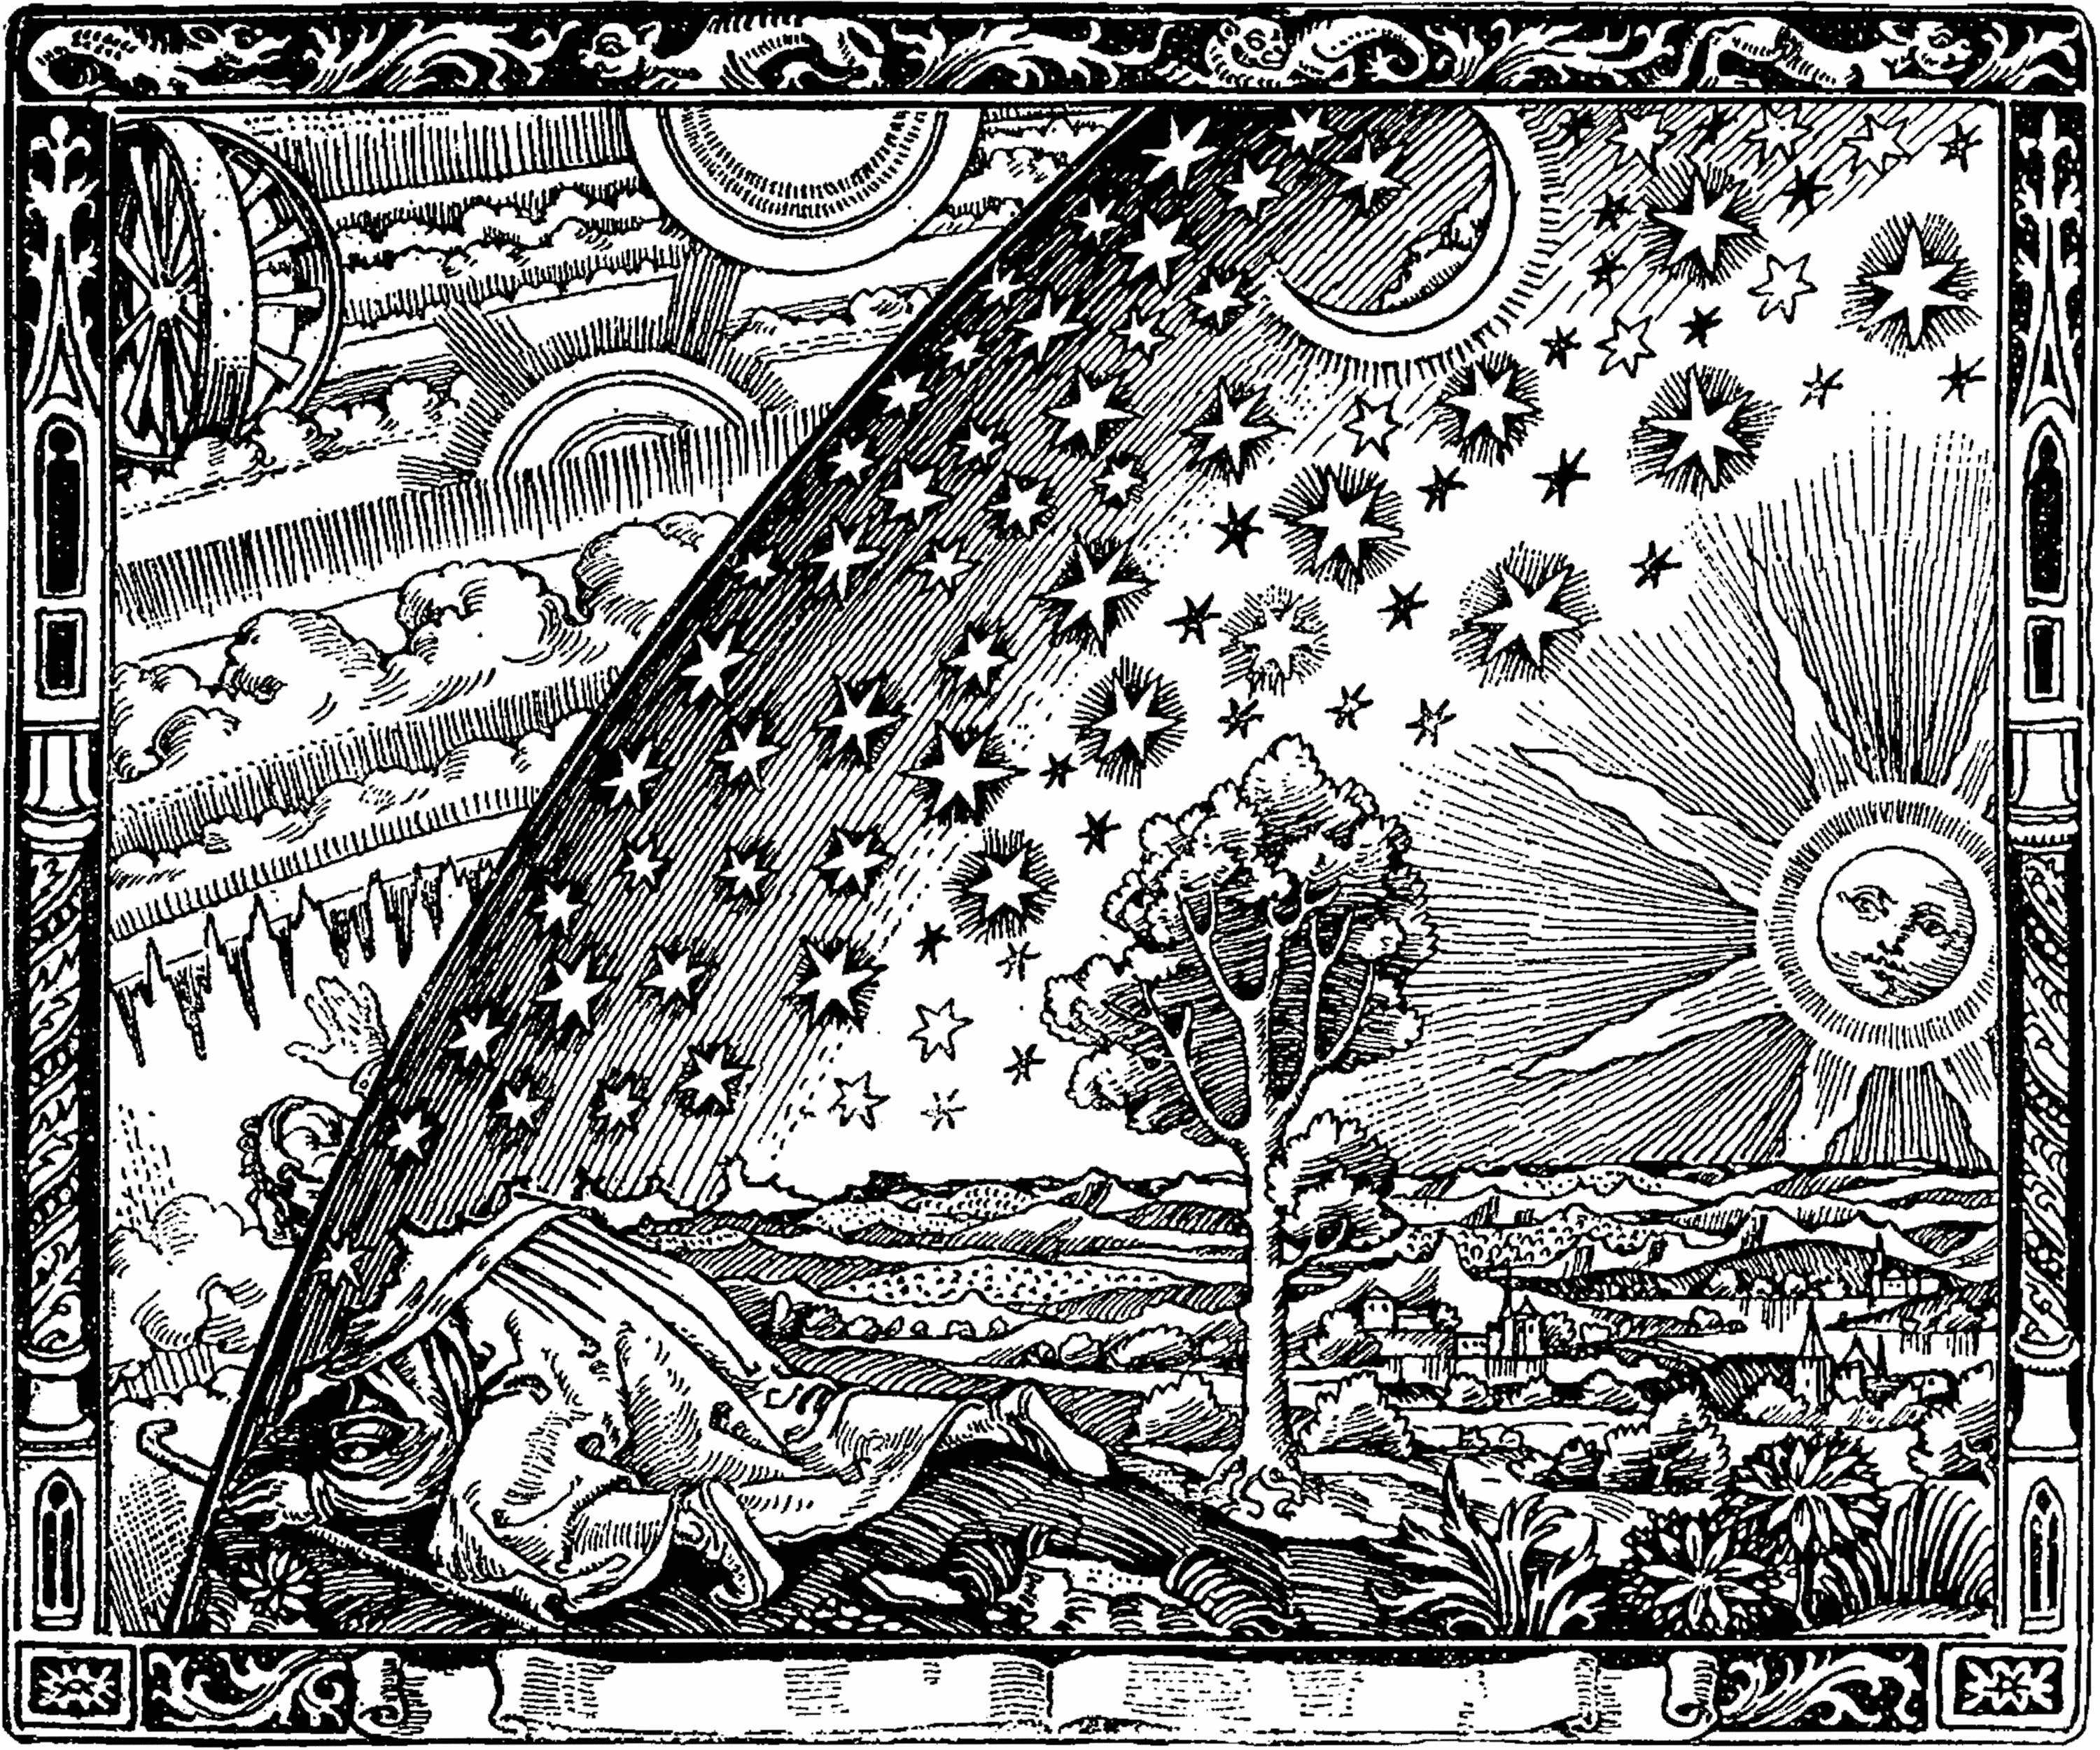
\includegraphics[width=0.9\textwidth]{flammarion}
%\caption{\textit{Flammarion gravure}. 1888.}
%\end{figure}

%\begin{figure}[h]
%\centering
%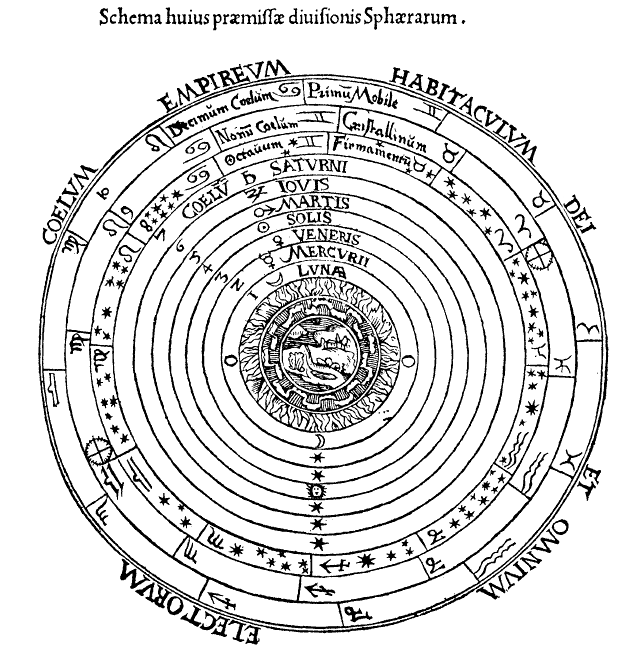
\includegraphics[width=0.9\textwidth]{Ptolemaicsystem-small}
%\caption{\textit{Schema huius praemissae divisionis sphaerarum.}}
%\end{figure}

%\newpage

\section{De wetten van Kepler}

Johannes Kepler (1571 - 1630) destilleerde uit de enorme hoeveelheid meetgegevens van planeetposities die Tycho Brahe (1546 - 1601) verzamelde, zijn drie wetten. Ze luiden: een planeet beweegt in een elliptische baan met de zon in een van de brandpunten, de voerstraal snijdt in gelijke tijdsintervallen gelijke oppervlakten (perken) uit (perkenwet) en de verhouding van het kwadraat van de periode tot de derde macht van de halve lange as van de ellipsbaan is voor alle planeten gelijk.

\section{De universele gravitatiekracht}

%- redenering maan

%- verklaring wetten Kepler

Isaac Newton (1642 - 1727) kon aantonen dat wanneer hij aannam dat planeten door de zon werden aangetrokken door een kracht die omgekeerd evenredig is met het kwadraat van de afstand, de drie wetten van Kepler hieruit af te leiden zijn. Daar waar de wetten van Kepler slechts inductief uit empirische gegevens zijn afgeleid, zijn ze bij Newton een gevolg van zijn bewegingsleer: de gravitatiekracht als oorzaak van beweging en zijn tweede wet als bewegingsvergelijking. Nu zijn de wetten een deductief gevolg uit een theoretisch model.

Een ander argument dat Newton gebruikte om zijn voorstel voor de formule van de universele gravitatiekracht te corroboreren\footnote{Een moeilijk woord dat `met argumenten staven' betekent.}, was een redenering over de versnelling van de maan.\footnote{Zijn berekeningen borg hij op omdat ze niet strookte met de realiteit. Enkele jaren later bleek echter dat de door astronomen gebruikte afstand tot de maan fout was. Een nieuwe waarde toonde aan dat Newton een correcte redenering had gebruikt.} Ze gaat als volgt. De maan maakt een nagenoeg cirkelvormige beweging. Haar versnelling is dus te berekenen met de formule voor de versnelling van een ECB. We hebben dan de omlooptijd en de afstand tot de maan nodig. De straal van de cirkelbeweging van de maan is ongeveer 60 keer de straal van de aarde.
\begin{eqnarray*}
	a&=&r\omega^2=r\left(\frac{2\pi}{T}\right)^2\\
	&=&6370\cdot10^3\rm\,m\cdot60\cdot\left(\frac{2\pi}{27,3\cdot24\cdot60\cdot60\rm\,s}\right)^2=0,0027\rm\,m/s^2
\end{eqnarray*}
Dit getal komt overeen met een omgekeerd kwadratische afhankelijkheid van de straal. Nemen we namelijk de valversnelling op aarde, $9,81\rm\,m/s^2$ en delen we deze door $60^2$ (de maan bevindt zich immers 60 keer zo ver), dan krijgen we hetzelfde getal.
\begin{eqnarray*}
	a=\frac{9,81\rm\,m/s^2}{60^2}=0,0027\rm\,m/s^2
\end{eqnarray*}
Hiermee had Newton een argument om aan te nemen dat de gravitatiekracht omgekeerd evenredig moet zijn met het kwadraat van de onderlinge afstand tussen de massa's.

De \textit{universele of algemene gravitatiekracht}, \'e\'en van de vier fundamentele natuurkrachten, wordt als volgt geformuleerd:
\begin{center}
\framebox{
\begin{minipage}[t]{\textwidth}
Twee puntmassa's $m$ en $m'$, die zich op een afstand $r$ van elkaar
bevinden, trekken elkaar aan met een kracht die gericht is volgens
de verbindingslijn van de twee massa's en waarvan de grootte recht
evenredig is met het product van de twee massa's en omgekeerd
evenredig met het kwadraat van de afstand tussen beide:
\begin{eqnarray}\label{universele gravitatiekracht}
F&=&G\frac{mm'}{r^2}
\end{eqnarray}
De evenredigheidsco\"effici\"ent $G$ wordt de
\textit{gravitatieconstante} genoemd.
\begin{eqnarray}\label{gravitatieconstante}\nonumber
G&=&6,67\cdot10^{-11}\rm\,\frac{Nm^2}{kg^2}
\end{eqnarray}
\end{minipage}}
\end{center}

Newton bepaalde de constante $G$ niet zelf. Dat werd na zijn dood door Cavendish (1731 - 1810) gedaan.

\newpage

\section{Satellietbanen}

Hoe komt het dat de maan door de aarde wordt aangetrokken en er toch niet naartoe valt? Dat komt omdat de neiging van de maan om door de traagheid weg te vliegen volgens de richting waarin hij beweegt, de valbeweging naar de aarde toe compenseert. De gravitatiekracht zorgt voor de middelpuntzoekende kracht van de nagenoeg cirkelvormige beweging die de maan maakt rond de aarde.\footnote{Maar welke kracht duwt de maan dan voort om zijn snelheid te onderhouden? Geen kracht! Herinner je dat de wet van de traagheid zegt dat je geen kracht nodig hebt om een eenmaal verworven snelheid aan te houden. Er is ook geen directe maar een indirecte relatie tussen kracht en snelheid. De tweede wet van Newton relateert kracht aan \textit{versnelling}, niet aan snelheid! Omdat er in de ruimte geen wrijving is, is er niemand om de maan tegen te houden en blijft hij voortgaan.}

Net zoals de maan worden ook kunstsatellieten door de gravitatiekracht in een baan rond de aarde gehouden. Denk maar aan GPS-satellieten en het internationaal ruimtestation. Op de website van de NASA\footnote{\href{http://science.nasa.gov/iSat/}{iSat: Interactive Satellite Viewer (science.nasa.gov/iSat/)}} kan je real-time gegevens van verschillende satellieten terugvinden.

\subsection{Parkeerbaan}

Met een satelliet is het net zoals met de maan. Willen we ervoor zorgen dat de satelliet steeds in eenzelfde baan ronde de aarde blijft cirkelen, dan moet hij een welbepaalde snelheid meekrijgen. Voor een cirkelvormige baan met de aarde als middelpunt fungeert de gravitatiekracht als middelpuntzoekende kracht. De versnelling is dan die van een ECB, wat we kunnen gebruiken om de juiste snelheid af te leiden:
\begin{eqnarray*}
F&=&ma\\
G\frac{m_am}{r^2}&=&m\frac{v^2}{r}\\
v&=&\sqrt{\frac{Gm_a}{r}}
\end{eqnarray*}
Hierin is $m$ de massa van de satelliet, $m_a$ de massa van de aarde en $r$ de straal van de cirkelbeweging die de satelliet maakt. De massa van de satelliet speelt duidelijk geen rol. 

Passen we deze formule toe op het internationaal ruimtestation, dat ongeveer op een hoogte van $412\rm\,km$ vliegt, dan krijgen we, met een gemiddelde aardstraal van $6370\rm\,km$, volgende schatting voor de snelheid:
\begin{eqnarray*}
	v=\sqrt{\frac{6,67\cdot10^{-11}\rm\,\frac{Nm^2}{kg^2}\cdot5,9721986\cdot10^{24}\rm\,kg}{6370\cdot10^3\rm\,m+412\cdot10^3\rm\,m}}=7,66\rm\,km/s
\end{eqnarray*}
Dit ligt erg dicht bij de eigenlijke snelheid -- en dat voor zo'n `simpele' berekening. De mechanica van Newton is duidelijk heel krachtig!

\subsection{Geostationaire baan}

Er is \'e\'en satellietbaan die een speciale eigenschap heeft: de snelheid van de satelliet en de afstand tot de aarde zijn zodanig dat de hoeksnelheid van de satelliet gelijk is aan die van de aarde. De baan ligt bovendien in het equatoriaal vlak zodat voor een waarnemer op de evenaar de satelliet steeds zichtbaar is in het zenit -- loodrecht boven de waarnemer. Vandaar dat over een geostationaire baan wordt gesproken.

Als we eisen dat de hoeksnelheid van de satelliet gelijk is aan die van de aarde (de periode moet bijgevolg 24 uur zijn) en dat de baan in het evenaarsvlak ligt, kunnen we de straal van de baan afleiden:
\begin{eqnarray*}
F&=&ma\\
&\Downarrow&\\
G\frac{m_am}{r^2}&=&mr\omega^2\\
r&=&\sqrt[3]{\frac{Gm_a}{\omega^2}}=\sqrt[3]{\frac{Gm_aT^2}{4\pi^2}}\\
&=&\sqrt[3]{\frac{6,67\cdot10^{-11}\rm\,\frac{Nm^2}{kg^2}\cdot5,9721986\cdot10^{24}\rm\,kg\cdot(24\cdot60\cdot60\rm\,s)^2}{4\pi^2}}\\
&=&42\,232\rm\,km
\end{eqnarray*}
Als we hier de straal van de aarde nog afhalen, vinden we dat de satellietbaan zich $42\,232\rm\,km-6\,370\rm\,km=35\,862\rm\,km$ boven het aardoppervlak bevindt. Dat is ongeveer een tiende van de afstand tot de maan.

\textit{Opmerking}: waarom kan er geen geostationaire baan boven Belgi\"e worden ge\"installeerd? Omdat alle parkeerbanen als middelpunt het middelpunt van de aarde moeten hebben. Het is immers de gravitatiekracht die voor de middelpuntzoekende kracht zorgt. Moest je een baan boven Belgi\"e willen maken, dan zou het middelpunt op de rotatieas ergens boven de noordpool liggen. Vanuit dat middelpunt wordt echter geen kracht uitgeoefend.


\section{Gewicht}

%- insteek via gewichtloos zijn in de ruimte

%- gewicht is hoeveel het weegt, de impact. Weegschaal?... Afwegen? Belang van iets, gewichtig? > voetnoot

%\begin{center}
\framebox{
\begin{minipage}[t]{\textwidth}
Het gewicht van een lichaam is de grootte van de kracht die door het lichaam op haar steun wordt uitgeoefend.
\end{minipage}}
%\end{center}

Let op het feit dat het om de \textit{grootte} van een kracht gaat en dat gewicht dus wordt uitgedrukt in newton. In de omgangstaal zijn we hierin niet correct. Men zegt zoveel kilogram te wegen terwijl kilogram de eenheid van massa is.

%- voorbeeld met een lift.


\section{De zwaartekracht}
De zwaartekracht is een bijzonder geval van de universele gravitatiekracht: de gravitatiekracht door de aarde op een massa uitgeoefend noemen we ook de zwaartekracht.

\subsection{De valversnelling}

Proefondervindelijk zien we dat op de aarde alle lichamen met
dezelfde valversnelling $g$ naar de aarde toe vallen. De tweede wet
van Newton zegt dan dat de zwaartekracht die deze versnelling moet
veroorzaken gelijk moet zijn aan de massa van het lichaam
vermenigvuldigd met deze versnelling:
%\begin{eqnarray*}
%F_z&=&mg
%\end{eqnarray*}
%Deze vergelijking geeft dus aan \textit{hoe groot} de kracht moet
%zijn. Het \textit{is} echter de universele gravitatiekracht door de
%aarde op de massa uitgeoefend. Er moet dus gelden:
\begin{eqnarray}
F&=&ma\nonumber\\
&\Downarrow&\nonumber\\
G\frac{m_Am}{r^2}&=&mg\nonumber\\
&\Updownarrow&\nonumber\\
g&=&G\frac{m_A}{r^2}
\end{eqnarray}
De valversnelling $g$ is inderdaad onafhankelijk van de massa van
het be\-schouw\-de lichaam.

De zwaartekracht op een grotere massa is wel groter, maar doordat
een grotere massa een grotere traagheid heeft, is het moeilijker haar
bewegingstoestand te veranderen. Deze twee eigenschappen heffen
elkaar dus op zodat alle massa's met een zelfde valversnelling vallen.

%\subsection{$g$ is geen constante}

%- factoren die $g$ be\"invloeden

%- welke benadering hebben we eigenlijk gemaakt?

%\clearpage
%\newpage

%\cleardoublepage
%!TEX root = ../fys_cursus.tex

\chapter{Arbeid \& Energie}

In essentie hebben we met de wetten van Newton, de formule voor o.a. de gravitatiekracht en de kinematica voldoende om alle mechanische verschijnselen te beschrijven. Je zou dus kunnen zeggen dat we geen bijkomende elementen nodig hebben. Maar wat met het begrip energie, een fundamentele grootheid in de fysica en vaak handig bij het oplossen van probleemstellingen?  Willen we dit begrip in de mechanica gebruiken, dan zullen we het moeten defini\"eren aan de hand van begrippen die we al hebben -- zoals kracht. De wetten van Newton vormen immers het fundament van de mechanica -- alles moet hierop gestoeld zijn. 

Je leerde ooit iets over energie: \textit{een lichaam bezit energie als het de mogelijkheid heeft om arbeid te verrichten.} Zo bezit een bewegende hamer \textit{kinetische energie} omdat hij als gevolg van zijn beweging arbeid kan verrichten: hij kan een nagel in de muur drijven. De opgewonden veer
van een mechanisch horloge is een voorbeeld van \textit{potenti\"ele energie}. Als gevolg van de spanningstoestand van de veer -- die door een bepaalde plaats wordt gekarakteriseerd -- kan de veer arbeid verrichten: terwijl de veer zich geleidelijk ontspant, verricht ze arbeid door de wijzers te laten ronddraaien. %De veer verkreeg zijn potenti\"ele energie doordat degene die het horloge opwond er arbeid op leverde.

Ook in de omgangstaal kennen we de termen arbeid en energie. Je mag echter niet vergeten dat deze hier een bredere betekenis dragen dan degene die we binnen de fysica voor ogen hebben. Zo moet de \textit{kwalitatieve} omschrijving van de mogelijkheid om arbeid te verrichten, vervangen worden door een \textit{kwantitatieve}; we willen weten \textit{hoeveel} arbeid er geleverd wordt, of \textit{hoeveel} energie een bepaald lichaam bezit. Als we bovendien zeggen dat energie de mogelijkheid is om arbeid te leveren, dan moeten we in eerste instantie het begrip arbeid \textit{defini\"eren}. We gebruiken hiervoor o.a. het begrip kracht. Aan de hand van het begrip arbeid, kunnen we dan vervolgens het begrip energie defini\"eren.

\section{Arbeid geleverd door een constante kracht}

%\subsection{Kracht en verplaatsing hebben dezelfde richting}
De arbeid $W$ door een constante kracht $F$ geleverd op een lichaam bij een verplaatsing $\Delta x=x_b-x_a$ wordt gedefinieerd als \footnote{Besef dat dit een \textit{definitie} van een fysische grootheid is. Terecht zou ge u kunnen afvragen waarom we arbeid op deze manier defini\"eren en niet anders. Dat de grootheid kracht erin moet voorkomen, is duidelijk: anders kan je een veer van een horloge niet opwinden. Ook is een verplaatsing nodig om van arbeid te kunnen spreken. Als immers de veer niet beweegt, kan er geen sprake zijn van een verandering in de energietoestand van de veer en dus ook niet van een overdracht van energie naar de veer -- wat arbeid is. Dat er bijvoorbeeld geen snelheid in voorkomt, kan je inzien door je te realiseren dat de snelheid waarmee je een veer opwindt, niet mag uitmaken. Enkel de uiteindelijke toestand van de veer is van belang. En waarom dan het product van de kracht met de verplaatsing? Wel, omdat het de enige manier is waarop we aan een fysische grootheid zullen komen die de naam energie waardig is... (!). Zie hiervoor het arbeid-energietheorema.}
\begin{eqnarray}
W&=&F\Delta x
\end{eqnarray}
Hierbij moeten kracht en verplaatsing dezelfde richting hebben. De SI-eenheid van arbeid is de joule:
\begin{eqnarray*}
[W]&=&[F]\cdot[\Delta x]=\rm N\cdot m=J
\end{eqnarray*}
%\subsection{Kracht en verplaatsing; verschillende rich\-ting}
Indien de beschouwde kracht en de verplaatsing niet dezelfde richting hebben, wordt alleen de component van de kracht volgens de verplaatsing in rekening gebracht. Er is namelijk geen beweging geassocieerd met de component loodrecht op de verplaatsing.
\begin{figure}[h]
\begin{center}
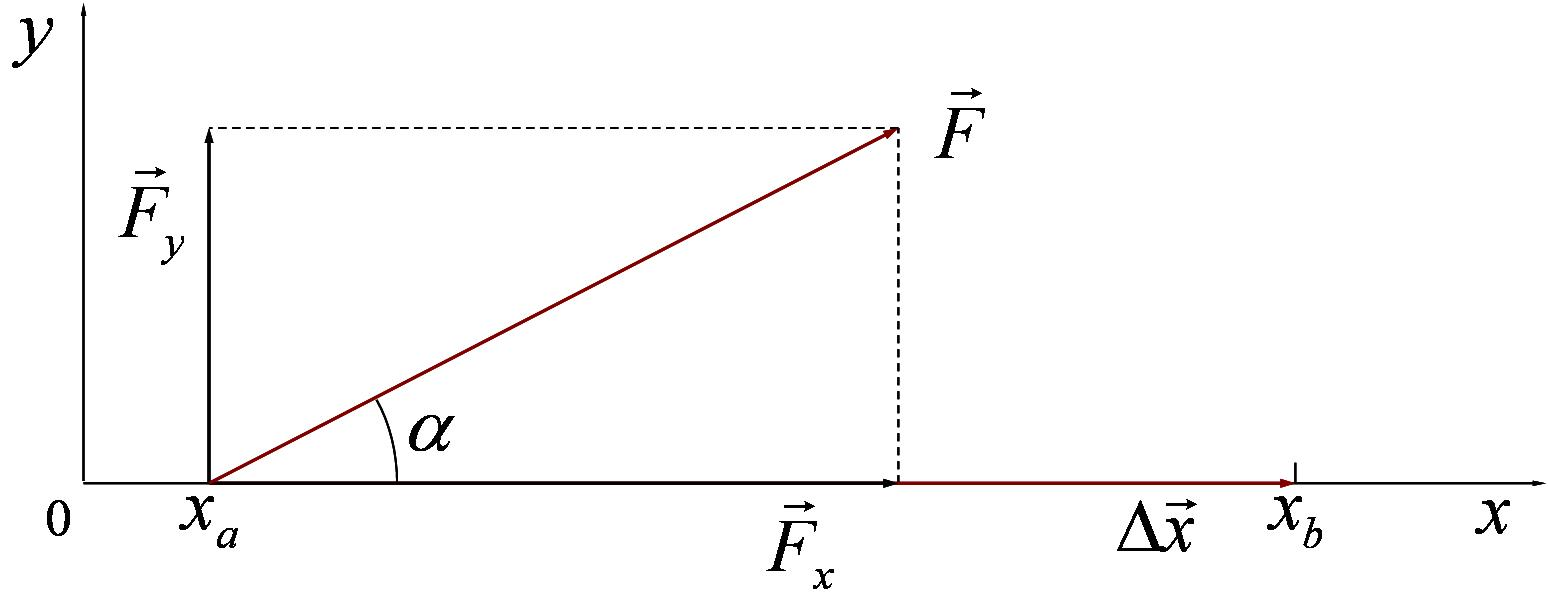
\includegraphics[width=0.7\textwidth]{arbeid_verschillende_richting}
\caption{kracht en verplaatsing met een verschillende richting}
\end{center}
\end{figure}

Als $\alpha$ de hoek tussen de kracht en de verplaatsing is, dan is de getalcomponent volgens de bewegingszin te schrijven als $F\cos{\alpha}$ en de arbeid door deze component geleverd als $W=F\cos{\alpha}\Delta x$. Dit laatste is niets anders dan het scalair product tussen de kracht en de verplaatsing.

De mechanische arbeid $W$, geleverd door een constante kracht $\vec{F}$, is gelijk aan het scalair product van de kracht met de verplaatsing:
\begin{eqnarray}
W&=&\vec{F}\cdot\Delta\vec{x}\label{def_arbeid_cste_kracht}
\end{eqnarray}

\section{Arbeid van een niet-constante kracht}

Algemeen zal een kracht gedurende de verplaatsing niet constant blijven. Ze zal met andere woorden o.a. afhankelijk zijn van de plaats waar het lichaam zich bevindt. We kunnen die afhankelijkheid beschrijven met behulp van een functie, de (grootte van de) kracht
als functie van de plaats:
\begin{eqnarray*}
F&=&F(x)
\end{eqnarray*}
Eenvoudigheidshalve beperken we ons hier tot bewegingen op een rechte. Bewegingen in meerdere dimensies vereisen een uitgebreidere integraaltheorie dan hetgeen we nu kennen.

We geven een opbouw om tot een definitie van arbeid te komen in het geval dat de kracht dus niet constant is. Ze vertoont gelijkenissen met de opbouw van de integraal.
\begin{figure}[h]
\centering
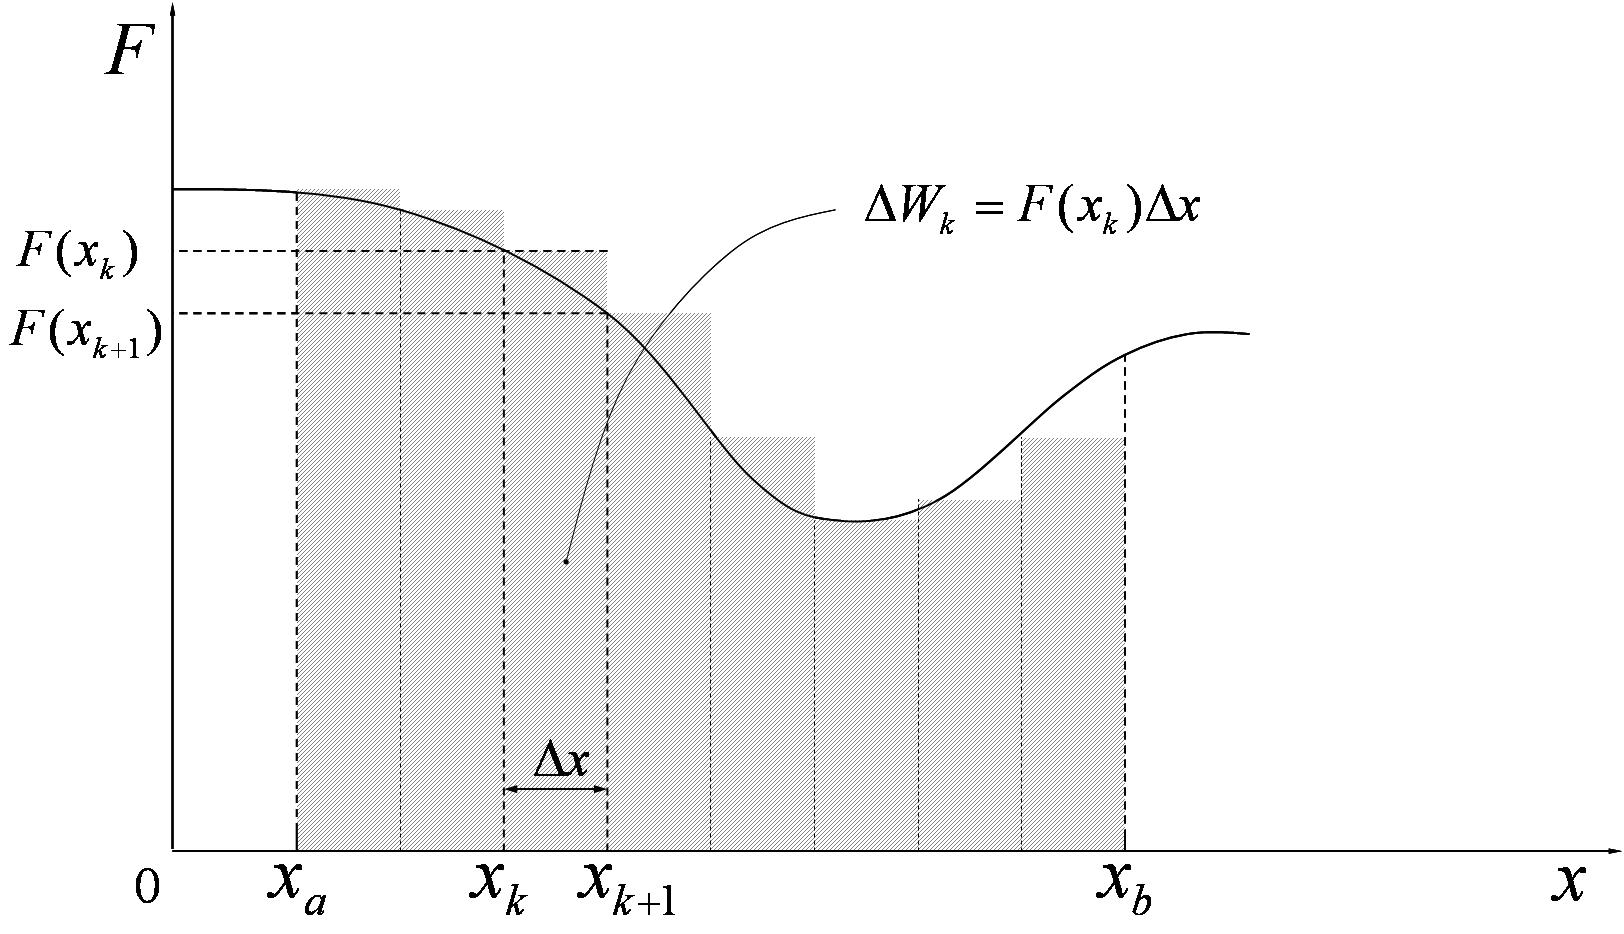
\includegraphics[width=0.85\textwidth]{arbeid_nietconstantekracht}
\caption{Opbouw arbeid bij een niet-constante kracht}
\end{figure}

Verdeel de verplaatsing $x_b-x_a$ in heel veel hele kleine stukjes $\Delta x$ bijvoorbeeld als volgt:
\begin{eqnarray*}
\Delta x&=&\frac{x_b-x_a}{n}
\end{eqnarray*}
met $n\in\mathbb{N}_0$ zeer groot. De posities tussen de stukjes kunnen we dan be\-schrij\-ven door
\begin{eqnarray*}
x_k=x_a+k\Delta x\ \ k\in\{0,1,2,\ldots,n\}
\end{eqnarray*}
Hoe kleiner $\Delta x$ is, hoe minder de kracht binnen deze stukjes vari\"eert en hoe meer dus $F(x_k)$ de kracht weergeeft die aanwezig is bij de verplaatsing van $x_{k}$ naar $x_{k+1}$. Het kleine stukje arbeid $\Delta W_k=F(x_k)\Delta x$ zouden we kunnen beschouwen als
een benadering van de geleverde arbeid gedurende deze kleine verplaatsing. De arbeid geleverd bij de gehele verplaatsing zou dan overeen kunnen komen met de som van alle stukjes geleverde arbeid. Hoe kleiner we $\Delta x$ nemen hoe meer die som overeenkomt met wat de totale arbeid zou moeten zijn, vandaar dat in de limiet van $\Delta x$ gaande naar nul, we de geleverde arbeid zouden kunnen vinden. Deze limiet komt overeen met het nemen van een integraal:
\begin{eqnarray*}
W\,=\,\lim_{\Delta x\rightarrow0}\sum_{k=0}^{n-1}\Delta W_k
%&=&\lim_{n\rightarrow\infty}\sum_{k=0}^{n-1}F(x_k)\Delta x\\
\,=\,\lim_{n\rightarrow\infty}\sum_{k=0}^{n}F(x_k)\Delta x
\,=\,\int_{x_a}^{x_b}F(x)~dx
\end{eqnarray*}
Dit moet de volgende algemene definitie van arbeid legitimeren.

\kader{De mechanische arbeid $W$, geleverd door een kracht $\vec{F}(x)$ gedurende de verplaatsing op een rechte van $x_a$ tot $x_b$ wordt gedefinieerd als
\begin{eqnarray}\label{W}
W=\int_{x_a}^{x_b}F_x(x)\ dx
\end{eqnarray}
waarbij $F_x(x)$ de getalcomponent van $\vec{F}(x)$ is volgens de bewegingsrichting.}

\textit{Opmerkingen:}
\begin{enumerate}
\item[-]Indien de kracht als functie van de plaats expliciet gekend is, kan de integraal verder bepaald worden.
\item[-]De twee vorige definities zijn speciale gevallen van deze definitie. Inderdaad bekomen we de formule (\ref{def_arbeid_cste_kracht}) indien de kracht een constante is. De kracht schuift voor het integraalteken en de integraal zelf wordt de verplaatsing.\footnote{Ga dit na!}
\item[-]Arbeid kan negatief zijn. Dit is o.a. het geval wanneer kracht en verplaatsing een tegengestelde zin hebben.
\end{enumerate}

\label{voorbeeld Hooke}
\voorbeeld{Arbeid door een veer geleverd}{\textsf{Een eenvoudig maar duidelijk voorbeeld van een kracht die afhankelijk is van de plaats is de kracht door een veer uitgeoefend. Voor niet te grote uitwijkingen wordt deze gegeven door de wet van Hooke:}
\begin{eqnarray*}
F(x)=-kx
\end{eqnarray*}
\textsf{Hierin is $k$ de veerconstante en $x$ de verlenging van de veer t.o.v. zijn evenwichtspositie~\footnote{Uit het vierde jaar ken je deze uitdrukking onder de vorm $F=k\Delta l$.}. Het minteken komt van het feit dat de kracht steeds tegengesteld is aan de uit\-wij\-king. Het is een \textit{terugroepkracht}. Bij het samendrukken van de veer bijvoorbeeld is $x<0$ zodat de kracht positief en dus tegengesteld aan de uitwijking is.}
\begin{figure}[h]
\centering
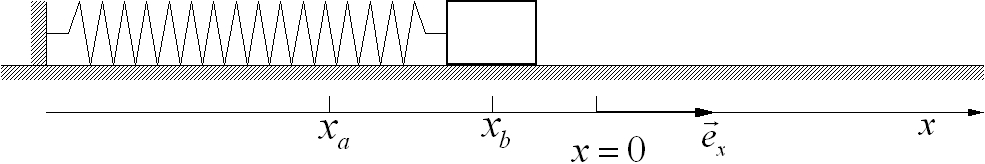
\includegraphics[width=0.85\textwidth ,angle=0]{elastische_energie}
\end{figure}

\textsf{We willen de arbeid berekenen door de veerkracht geleverd op een massa bij de verplaatsing van een verlenging $x_a$ naar een verlenging $x_b$. Volgens de definitie wordt dit:}
\begin{eqnarray*}
W\,=\,\int_{x_a}^{x_b}F(x)~dx&=&\int_{x_a}^{x_b}-kx~dx\\
&=&-k\left[\frac{x^2}{2}\right]_{x_a}^{x_b}\\
&=&\frac{1}{2}k{x_a}^2-\frac{1}{2}k{x_b}^2
\end{eqnarray*}
\textsf{Indien het beginpunt $x_a$ verder uit de evenwichtspositie ligt dan het eindpunt $x_b$ is de geleverde arbeid positief.}}

%\section{Vermogen}
%Dit onderdeel hoef je niet te kennen.
\section{Het arbeid-energietheorema}

Indien op een voorwerp een resulterende kracht inwerkt, moet de snelheid ervan veranderen. Volgens de tweede wet van Newton krijgt het immers een versnelling. Indien kracht en verplaatsing dezelfde zin hebben, is er een snelheidstoename en is de arbeid door de kracht geleverd positief. Er moet dus misschien een verband bestaan tussen de geleverde arbeid en de verandering in snelheid \ldots 

\kader{\textit{Het arbeid-energietheorema}

Voor de arbeid door de \textit{resulterende kracht} op een voorwerp geleverd geldt:
\begin{eqnarray}
W=\int_{x_a}^{x_b}F(x)\
dx=\frac{mv_b^2}{2}-\frac{mv_a^2}{2}\nonumber
\end{eqnarray}
waarin $m$ de massa van het voorwerp is en $v_a$ en $v_b$ de snelheden van het voorwerp op respectievelijk het begin- en het eindpunt.

In het rechterlid verschijnt een grootheid die we \textit{defini\"eren} als de \mbox{\textit{kinetische energie}} van het voorwerp:
\begin{eqnarray}
E_k&=&\frac{mv^2}{2}\nonumber
\end{eqnarray}
De arbeid geleverd door de resulterende kracht op een voorwerp, is dus gelijk aan het verschil van de kinetische energie van het lichaam in begin- en eindpunt:
\begin{eqnarray}
W&=&E_{k,b}-E_{k,a}
\end{eqnarray}}

\textit{Opmerkingen:}
\begin{enumerate}
\item[-]Dit theorema geeft een samenhang tussen arbeid en energie
zoals we dat verwachten. De \textit{nettoarbeid} geleverd over het hele traject \textit{door} de resulterende kracht \textit{op} het voorwerp, resulteert in een toe- of afname van de
kinetische energie van dat voorwerp met \textit{eenzelfde waarde}.
Zoveel arbeid als geleverd wordt, zoveel energie krijgt of verliest het voorwerp. De manier waarop de arbeid is geleverd tussen begin- en eindpunt speelt geen rol. Enkel de totale hoeveelheid is van belang.
%\footnote{Indien een kracht arbeid zou leveren als ze
%loodrecht op de verplaasting zou staan, dan zou er arbeid kunnen zijn
%\textit{zonder} een toename in snelheid. M.a.w. zou dit theorema dan
%niet opgaan. De betekenis van arbeid zou dan verloren gaan.}

\item[-]Indien de geleverde nettoarbeid op een voorwerp positief is, neemt de
kinetische energie toe. Voor positieve arbeid hebben kracht en
verplaatsing tussen begin- en eindpunt meer eenzelfde dan een
tegengestelde zin zodat de snelheid inderdaad kan toenemen. Denk bijvoorbeeld aan een vallende steen; hier levert de zwaartekracht ook positieve arbeid.
\item[-]Indien de geleverde nettoarbeid op een
voorwerp negatief is, neemt de kinetische energie af. Voor een
negatieve arbeid hebben kracht en verplaatsing tussen begin- en
eindpunt meer een tegengestelde dan een gelijke zin. De snelheid zal op die manier kunnen afnemen. De geleverde arbeid op
bij\-voor\-beeld een hamer die een nagel in de muur drijft, is
negatief. Zijn snelheid, en dus zijn kinetische energie, is
afgenomen. Ze is gebruikt om de nagel in de muur te krijgen.
Inderdaad is de kracht \textit{door} de hamer op de nagel
uitgeoefend met de beweging mee (de \textit{hamer} levert positieve arbeid, en verliest energie) en is de reactiekracht, de kracht door de nagel \textit{op} de hamer uitgeoefend, tegengesteld
aan de beweging (de \textit{nagel} levert negatieve arbeid, of ontvangt dus energie).
\item[-]Merk op dat dit theorema geldt voor de arbeid door de
\textit{resulterende kracht} geleverd en in de regel niet door
slechts \'e\'en van de krachten die op het voorwerp werken. Het is
de resulterende kracht die voor een resulterende versnelling van het
lichaam zorgt en dus voor een verandering in de snelheid.
\end{enumerate}

\textit{Bewijs arbeid-energietheorema}

Veronderstel dat de resulterende kracht wordt gegeven door de functie $F(x)$. We berekenen de arbeid door de resulterende kracht geleverd wanneer het voorwerp een verplaatsing ondergaat van $x_a$ naar $x_b$ door de tweede wet van Newton te gebruiken\footnote{Het gaat hier immers over de resulterende kracht\ldots}, de kettingregel en een substitutie door te voeren.
\begin{eqnarray*}
W&=&\int_{x_a}^{x_b}F(x)dx\\
&=&\int_{x_a}^{x_b}ma\,dx\\
&=&\int_{x_a}^{x_b}m\frac{dv}{dt}dx
\end{eqnarray*}
Door de kettingregel $\frac{dv}{dt}=\frac{dv}{dx}\frac{dx}{dt}$ en de definitie van snelheid $v=\frac{dx}{dt}$ te gebruiken, krijgen we
\begin{eqnarray*}
W&=&\int_{x_a}^{x_b}m\frac{dv}{dx}\frac{dx}{dt}dx\\
&=&\int_{x_a}^{x_b}m\frac{dv}{dx}v\,dx\\
\end{eqnarray*}
Deze integraal kunnen we uitwerken door de substitutie $v=v(x)$ door te voeren\footnote{Omdat de substitutie met de letter $v$ enigszins verwarrend is, vind je onder de uitdrukking de benoeming van de variabelen zoals je die voor de substitutieregel kent, nl. met $u$. En hopelijk overbodig, hier de substitutieregel:
\begin{eqnarray*}
\int_{a}^{b}f(\underbrace{g(x)}_u)\underbrace{\underbrace{g'(x)}_{u'}\underbrace{dx}_{dx}}_{du}=\int_{g(a)}^{g(b)}f(u)du
\end{eqnarray*}}. De integratiegrenzen $x_a$ en $x_b$ voor de positie $x$, worden $v_a=v(x_a)$ en $v_b=v(x_b)$ voor de snelheid $v$. We wisselen voor de duidelijkheid ook twee factoren om.
\begin{eqnarray*}
W&=&\int_{x_a}^{x_b}m\underbrace{v\frac{dv}{dx}\,dx}_{u\cdot u'\,dx}\\
&=&\int_{v(x_a)}^{v(x_b)}mv\,dv\\
&=&\left[\frac{mv^2}{2}\right]_{v_a}^{v_b}\\
&=&\frac{mv_b^2}{2}-\frac{mv_a^2}{2}
\end{eqnarray*}
\phantom{}\hfill$\blacksquare$

\voorbeeld{Opgave arbeid-energie theorema}{\textsf{ Een horizontaal liggende veer op tafel heeft een veerconstante $k=360\rm\,N/m$ en wordt $11,0\rm\,cm$ ingedrukt. Een blok van $1,85\rm\,kg$ wordt tegen de gespannen veer gelegd en losgelaten. De wrijvingsco\"effici\"ent tussen het blok en de tafel is $0,38$.
\begin{enumerate}
\item Hoeveel arbeid levert de veerkracht vanaf de ingedrukte toestand tot in zijn evenwichtstoestand?
\item Hoeveel arbeid levert de wrijvingskracht over hetzelfde traject?
\item Hoe groot is de nettoarbeid?
\item Welke snelheid heeft het blok wanneer het zich, in de evenwichtstoestand, van de veer losmaakt?
\end{enumerate}
}}

%\newpage

\section{Potenti\"ele energie}

Naast kinetische energie -- de energie geassocieerd met de beweging van een lichaam -- kunnen we een andere vorm van mechanische energie defini\"eren: de \textit{potenti\"ele energie}. Dit is de energie geassocieerd met de plaats of configuratie van een lichaam. Een lichaam met kinetische energie heeft energie omdat het als gevolg van zijn beweging arbeid kan verrichten op een ander object. Kan een object arbeid verrichten als gevolg van zijn plaats, dan noemen we deze energie potenti\"ele energie.

Het leveren van arbeid op een voorwerp hoeft niet altijd te resulteren in een verandering van de kinetische energie. Bijvoorbeeld wanneer de arbeid van slechts \'e\'en van de krachten op een voorwerp wordt beschouwd en niet de arbeid door de resulterende kracht geleverd. De geleverde arbeid moet dan naar een andere vorm van energie gaan: potenti\"ele energie. Bij het opwinden van een horloge bijvoorbeeld wordt de geleverde arbeid gebruikt om de veer samen te drukken. De veer kan zich daarna ontspannen en arbeid op de wijzers leveren.

De vraag \textit{hoeveel} energie een voorwerp heeft, zal bij nader inzien enkel relatief kunnen worden bepaald. Is bijvoorbeeld de kinetische energie van een bekertje koffie op het tafeltje van de trein van Brussel naar Gent gelijk aan nul omdat het t.o.v. het tafeltje niet beweegt? Of is de kinetische energie verschillend van nul omdat het bekertje een snelheid heeft t.o.v iemand buiten de trein en dus, moest de trein plots stoppen, het bekertje verder zal vliegen en (veel opkuis-) arbeid kan leveren? En hoeveel energie heeft een blokje op een bepaalde hoogte? Zoveel als dat het arbeid kan leveren? Dat zal niet eenduidig te bepalen zijn. De geleverde arbeid tot op het tafeloppervlak, de grond of de bodem van de put die we vervolgens hebben gegraven is steeds verschillend. De geleverde arbeid, en dus de energie, is afhankelijk van het referentiepunt dat we nemen. In ieder geval moet de energie van een voorwerp afnemen met de hoeveelheid arbeid die het levert.

%Potenti\"ele energie is echter niet in alle gevallen te
%defini\"eren. In namelijk niet alle gevallen is de mogelijk te
%leveren hoeveelheid arbeid eenduidig bepaald.

%\newpage

\subsection{Elastische potenti\"ele energie}\label{elastische
potentiele energie}

We hernemen het voorbeeld van de veerkracht (\ref{voorbeeld Hooke}).
\begin{figure}[h]
\begin{center}
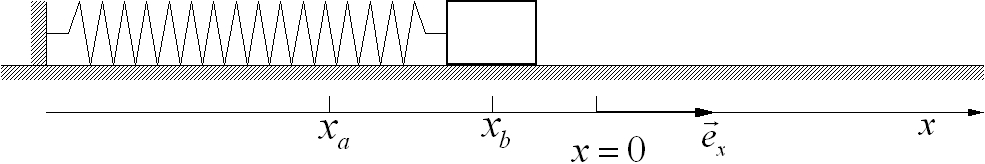
\includegraphics[width=0.8\textwidth ,angle=0]{elastische_energie}
\end{center}
\end{figure}
\newline
Hier vonden we dat de hoeveelheid arbeid door de veerkracht geleverd
bij een verplaatsing van $x_a$ naar $x_b$ gegeven wordt door:
\begin{eqnarray*}
W&=&\frac{1}{2}kx_ a^2-\frac{1}{2}kx_ b^2
\end{eqnarray*}
De geleverde arbeid kan geschreven worden als het verschil van de uitdrukking $\frac{1}{2}kx^2$ ge\"evalueerd in begin- en eindpunt. De waarde van de uitdrukking neemt af met de hoeveelheid arbeid die is geleverd. We kunnen de uitdrukking dus interpreteren als de hoeveelheid energie die de veer op een bepaald punt, een bepaalde plaats, bezit. Dat wat immers verloren gaat aan energie -- de oorspronkelijke energie min de overblijvende energie -- moet door de veer worden geleverd als arbeid. We noemen de uitdrukking de \textit{elastiche potenti\"ele energie} van een veer:
\begin{eqnarray}
E_p&=&\frac{1}{2}kx^2\label{Ep=1/2kx^2}
\end{eqnarray}
De geleverde arbeid kunnen we vervolgens schrijven als
\begin{eqnarray*}
W&=&E_{p,a}-E_{p,b}\,=\,-(E_{p,b}-E_{p,a})\\
&\Updownarrow&\\
W&=&-\Delta E_p
\end{eqnarray*}
Hierin is $\Delta E_p$ de verandering van potenti\"ele energie: $\Delta E_p=E_{p,\rm eind}-E_{p,\rm begin}$. Als de veer arbeid verricht dan gaat dat ten koste van haar potenti\"ele energie: is de geleverde arbeid $W$ positief, dan moet er een afname van de potenti\"ele energie zijn (de verandering $\Delta E_p$ moet negatief zijn). Opnieuw: de hoe\-veel\-heid geleverde arbeid komt overeen met het verlies in potenti\"ele energie tussen begin- en eindpunt. Is de verandering van de potenti\"ele energie $\Delta E_p$ positief dan is de geleverde arbeid negatief. Negatieve arbeid betekent dat i.p.v. het leveren van arbeid (het weggeven van energie), er van elders energie wordt toegevoegd en wordt omgezet in potenti\"ele energie.

\subsection{Gravitationele potenti\"ele energie}\label{gravitationele potentiele energie}

Beschouw een massa op een hoogte boven het aardoppervlak. Vanuit deze positie kan ze arbeid verrichten en zal ze dus potenti\"ele energie bezitten. Als we de massa bijvoorbeeld laten vallen kan ze op de grond een nagel inslaan en dus arbeid verrichten.
\begin{figure}[h]
\begin{center}
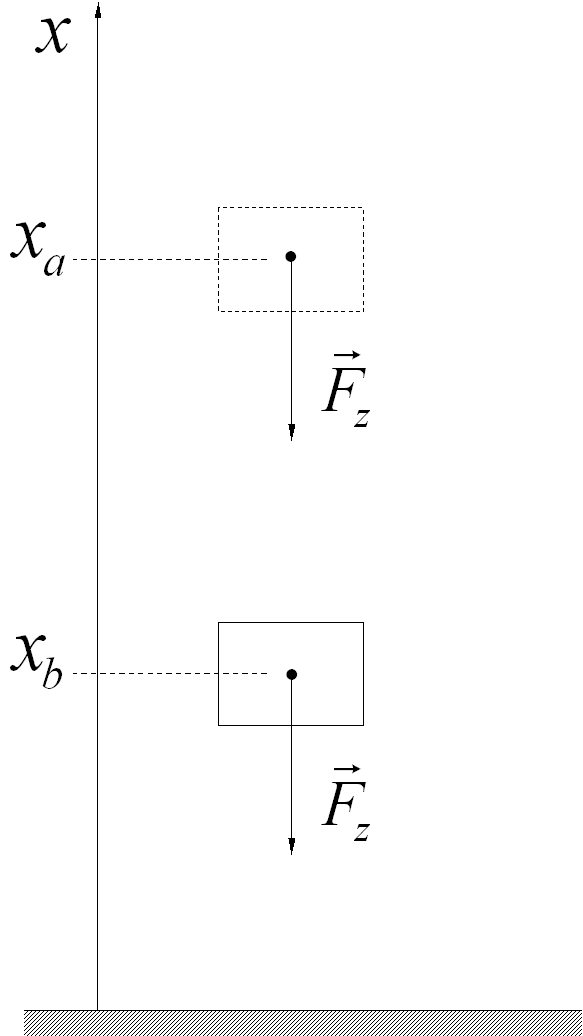
\includegraphics[height=5.5cm ,angle=0]{gravitationele_energie}
\end{center}
\end{figure}
Bij het vallen van een hoogte $x_a$ naar een hoogte $x_b$ levert de zwaartekracht die aan de massa trekt een arbeid gelijk aan:
\begin{eqnarray*}
W\,=\,\int_{x_a}^{x_b}F_zdx\,=\,\int_{x_a}^{x_b}(-mg)dx\,=\,mgx_a-mgx_b
\end{eqnarray*}
Hier voldoet de uitdrukking $mgx$ aan wat we verwachten van potenti\"ele ener\-gie. Het verschil van de uitdrukking ge\"evalueerd in het beginpunt en het eindpunt -- het verschil in energie -- is gelijk aan de hoeveelheid arbeid die tussen deze twee posities kan worden geleverd. We noemen de uitdrukking de \textit{gravitationele potenti\"ele energie}. En als we $x$ door $h$ vervangen, krijgen we de gekende vorm:
\begin{eqnarray}
E_p&=&mgh\label{Ep=mgh}
\end{eqnarray}
Net zoals bij de veerkracht geldt $W=-\Delta E_p$. 

Waarom nu eigenlijk dat minteken? Als de massa valt, wordt door de zwaartekracht positieve arbeid verricht. Op een punt iets lager dan waar de massa was vertrokken, kan de massa nog minder ver vallen zodat ze vanuit dit punt minder arbeid kan leveren. Haar potenti\"ele energie is afgenomen of de verandering $\Delta E_p$ is negatief. Dat wat aan potenti\"ele energie verloren is gegaan, is aan arbeid geleverd. Als de massa omhoog wordt gegooid, heeft ze in een punt hoger dan daar waar ze vertrok meer potenti\"ele energie. Vanaf een grotere hoogte kan ze meer arbeid leveren. De potenti\"ele energie neemt dus toe of de verandering $\Delta E_p$ is positief. De zwaartekracht $F_z$ is echter tegengesteld (naar beneden gericht) aan de verplaatsing (naar boven) zodat de geleverde arbeid negatief is. Het toenemen van de energie kan maar mogelijk zijn als van elders energie aan de massa wordt gegeven. In dit geval is ze afkomstig van de kinetische energie die bij het opwerpen wordt meegegeven.

Merk op dat de massa in staat is arbeid te verrichten als gevolg van het feit dat de zwaartekracht erop inwerkt en de massa bijgevolg \textit{zelf} een even grote kracht kan uitoefenen. Op die manier kunnen we de potenti\"ele energie toekennen aan de massa; \textit{de massa} gaat op deze manier in staat zijn arbeid te verrichten.

\subsection{Gravitationele potenti\"ele energie, algemeen}\label{gravitationele potentiele energie alg}

Beschouw een massa onderhevig aan de universele gravitatiekracht. We gaan opnieuw opzoek naar een potenti\"ele energiefunctie geassocieerd aan deze kracht.
\begin{figure}[h]
\begin{center}
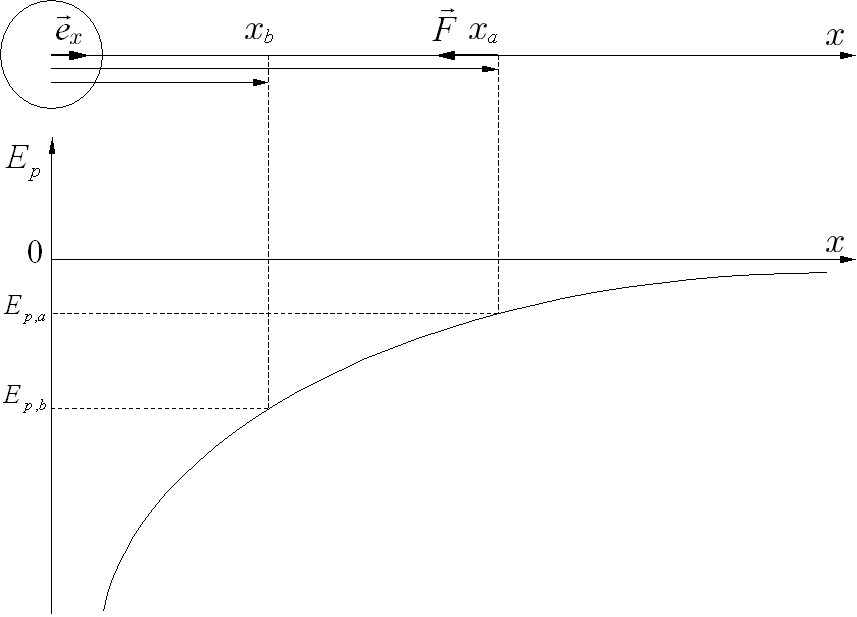
\includegraphics[width=0.9\textwidth ,angle=0]{gravitationele_energie_algemeen}
\end{center}
\end{figure}

Kiezen we een $x$-as met de oorsprong op de massa $m$ dan wordt, omdat de kracht steeds naar de oorsprong is gericht, de component van de universele gravitatiekracht op de massa $m'$ gegeven door
\begin{eqnarray*}
F(x)&=&-G\frac{mm'}{x^2}
\end{eqnarray*}
De arbeid die door de gravitatiekracht wordt geleverd bij de verplaatsing van de massa $m'$ van $x_a$ naar $x_b$ wordt dan:
\begin{eqnarray*}
W&=&\int_{x_a}^{x_b}-G\frac{mm'}{x^2}~{\rm d}x\\
&=&-Gmm'\int_{x_a}^{x_b}\frac{1}{x^2}~{\rm d}x\\
&=&-Gmm'\left[-\frac{1}{x}\right]_{x_a}^{x_b}\\
&\Updownarrow&\\
W&=&\left(-G\frac{mm'}{x_a}\right)-\left(-G\frac{mm'}{x_b}\right)
\end{eqnarray*}
De potenti\"ele energie voor een massa $m'$ wordt bijgevolg geven
door
\begin{eqnarray}
E_p&=&-G\frac{mm'}{x}\label{Ep=-Gmm'/x}
\end{eqnarray}

\subsection{Referentiepunt van de potenti\"ele energie}

Ai, de potenti\"ele energiefunctie (\ref{Ep=-Gmm'/x}) is voor alle waardes van $x$
\textit{negatief}. Zou potenti\"ele energie overeenkomen met de mogelijk te leveren hoeveelheid  arbeid, dan zou de massa met andere woorden minder dan geen arbeid kunnen leveren vanop een
bepaalde afstand. Een vallende steen op de aarde lijkt toch wel het tegendeel te bewijzen\ldots. Bovendien is de hoeveelheid arbeid die de massa $m'$ vanaf een bepaald punt tot aan $m$ kan leveren \textit{oneindig} groot \footnote{Waarom?}. De massa zou dus oneindig veel energie hebben. Zeggen dat de potenti\"ele energie gelijk is aan de hoeveelheid arbeid die kan worden verricht, is dus niet mogelijk?!

De potenti\"ele energie kan niet als een absolute maar enkel als een relatieve grootheid worden gedefinieerd. Het enige wat we van de potenti\"ele ener\-gie kunnen verwachten is dat het
\textit{verschil} tussen een begin- en eindpunt overeenkomt met de hoeveelheid geleverde arbeid tussen die twee punten.
%\begin{eqnarray*}
%W&=&-\Delta E_p
%\end{eqnarray*}
Een relatieve grootheid is tot op een constante na bepaald. Het gevolg is dat als $E_p$ een potenti\"ele energiefunctie is, $E_p'=E_p+\rm cte$ dat ook is. Immers:
\begin{eqnarray*}
E_{p,a}'-E_{p,b}'&=&(E_{p,a}+{\rm cte})-(E_{p,b}+{\rm cte})\\
&=&E_{p,a}-E_{p,b}\\
&=&W
\end{eqnarray*}
Bij de potenti\"ele energiefuncties (\ref{Ep=1/2kx^2}), (\ref{Ep=mgh}) en (\ref{Ep=-Gmm'/x}) zoals we ze hiervoor hebben gegeven, mag dus steeds een constante worden opgeteld. Het
\textit{re\-fe\-ren\-tiepunt} -- daar waar de potenti\"ele energie nul is -- kan vrij worden gekozen.

\subsection{Potenti\"ele energie}

Uit de drie voorbeelden blijkt dat in het algemeen de potenti\"ele
energie een plaatsafhankelijke functie moet zijn waarvan het
verschil tussen twee punten overeenkomt met de geleverde arbeid door
de kracht geassocieerd met deze functie. Noemen we deze functie
$U(x)$, dan moet gelden:
\begin{eqnarray*}
  W=\int_{x_a}^{x_b}F(x)~{\rm d}x &=&-(U(x_b)-U(x_a))\\
  &\Updownarrow&\\
  \int_{x_a}^{x_b}-F(x)~{\rm d}x &=&U(x_b)-U(x_a)\\
\end{eqnarray*}
Als $U(x)$ een primitieve functie voor $-F(x)$ is (dus een functie
waarvan de afgeleide de functie $-F(x)$ is: $U'(x)=-F(x)$) dan is
aan deze voorwaarde voldaan. Immers geldt dan:
\begin{eqnarray*}
\int_{x_a}^{x_b}-F(x)~{\rm d}x=\int_{x_a}^{x_b}\frac{d}{dx}U(x)~{\rm d}x&=&U(x_b)-U(x_a)\\
\end{eqnarray*}
Algemeen geldt dan ook voor de potenti\"ele energie:

\kader{Indien er voor een plaatsafhankelijke kracht $F(x)$ een functie $U(x)$ bestaat
waarvoor de afgeleide op een minteken na de kracht is,
\begin{eqnarray}\label{U(x)}
F(x)&=&-\frac{d}{dx}U(x)\nonumber
\end{eqnarray}
dan wordt $U(x)$ de \textit{potenti\"ele energie} genoemd.}

De potenti\"ele energie is dus een functie waarvoor de negatieve afgeleide de kracht is. Waarom een minteken? Een positieve afgeleide betekent een toename van de potenti\"ele energie. Om naar een hogere energie te gaan moet \textit{tegen} de kracht in worden bewogen. De kracht moet dus tegengesteld zijn aan de richting waarin de potenti\"ele enrgie toeneemt.

Zie ook dat de potenti\"ele energie inderdaad tot op een constante na is ge\-de\-fi\-ni\-eerd. Bij het afleiden valt immers een constante weg.

Een kracht waarvoor een potentiaalfunctie bestaat, levert arbeid die enkel bepaald wordt door begin- en eindpunt. De arbeid is dus onafhankelijk van de gevolgde weg. Zo'n kracht wordt conservatief genoemd. Enkel voor conservatieve krachten bestaat dus een potenti\"ele energie.

Ga na dat de energiefuncties die we bij de drie voorbeelden (\ref{gravitationele potentiele energie}), (\ref{elastische potentiele energie}) en (\ref{gravitationele potentiele energie
alg}) vonden, voldoen aan deze definitie en dus potenti\"ele energiefuncties zijn.

%\newpage

\section{Het beginsel van behoud van energie}\label{beginsel_behoud_energie}

Het arbeid-energietheorema relateert de geleverde arbeid door een resulterende kracht met de toename aan kinetische energie. Het zegt dat de hoeveelheid geleverde arbeid door de resulterende kracht volledig wordt gebruikt voor de toename van kinetische energie.
Anderzijds als met de resulterende kracht een potenti\"ele energie kan worden geassocieerd, dan is de geleverde arbeid afkomstig van het verlies in potenti\"ele energie. De energie die dus onder de vorm van potenti\"ele energie verloren gaat wordt in kine\-ti\-sche energie gewonnen. En dit zodanig dat de som van beide energi\"en - de totale mechanische energie - constant blijft.
\newline
\newline
Uit $W=\Delta E_k$ en $W=-\Delta E_p$ volgt:
\begin{eqnarray}
\Delta E_k&=&-\Delta E_p\nonumber\\
%&\Updownarrow&\nonumber\\
%E_{k,b}-E_{k,a}&=&E_{p,a}-E_{p,b}\nonumber\\
&\Updownarrow&\nonumber\\
E_{k,a}+E_{p,a}&=&E_{k,b}+E_{p,b}\nonumber
\end{eqnarray}
Spelen dus enkel krachten een rol waarvoor een potenti\"ele energie functie bestaat, dan is de som van de kinetische en de potenti\"ele energie van een voorwerp gedurende de beweging constant.

\kader{\textit{Het beginsel van behoud van mechanische energie}
\begin{eqnarray}
E_{k,a}+E_{p,a}&=&E_{k,b}+E_{p,b}\\
&\Updownarrow&\nonumber\\
E=\frac{mv^2}{2}+E_p~&=&~\mathrm{constant}
\end{eqnarray}\vspace{0cm}}

Het principe van behoud van energie is een van de meest fundamentele principes in de fysica \ldots 

%\clearpage
%\newpage

\cleardoublepage
\null\thispagestyle{empty}

\vfill

\begin{center}
\textsc{DEEL III}
\end{center}
\begin{center}
\textsc{\LARGE PERIODIEKE VERSCHIJNSELEN}
\end{center}

\vfill

\begin{center}
\begin{picture}(90,120)(0,0)
%\put(115,0){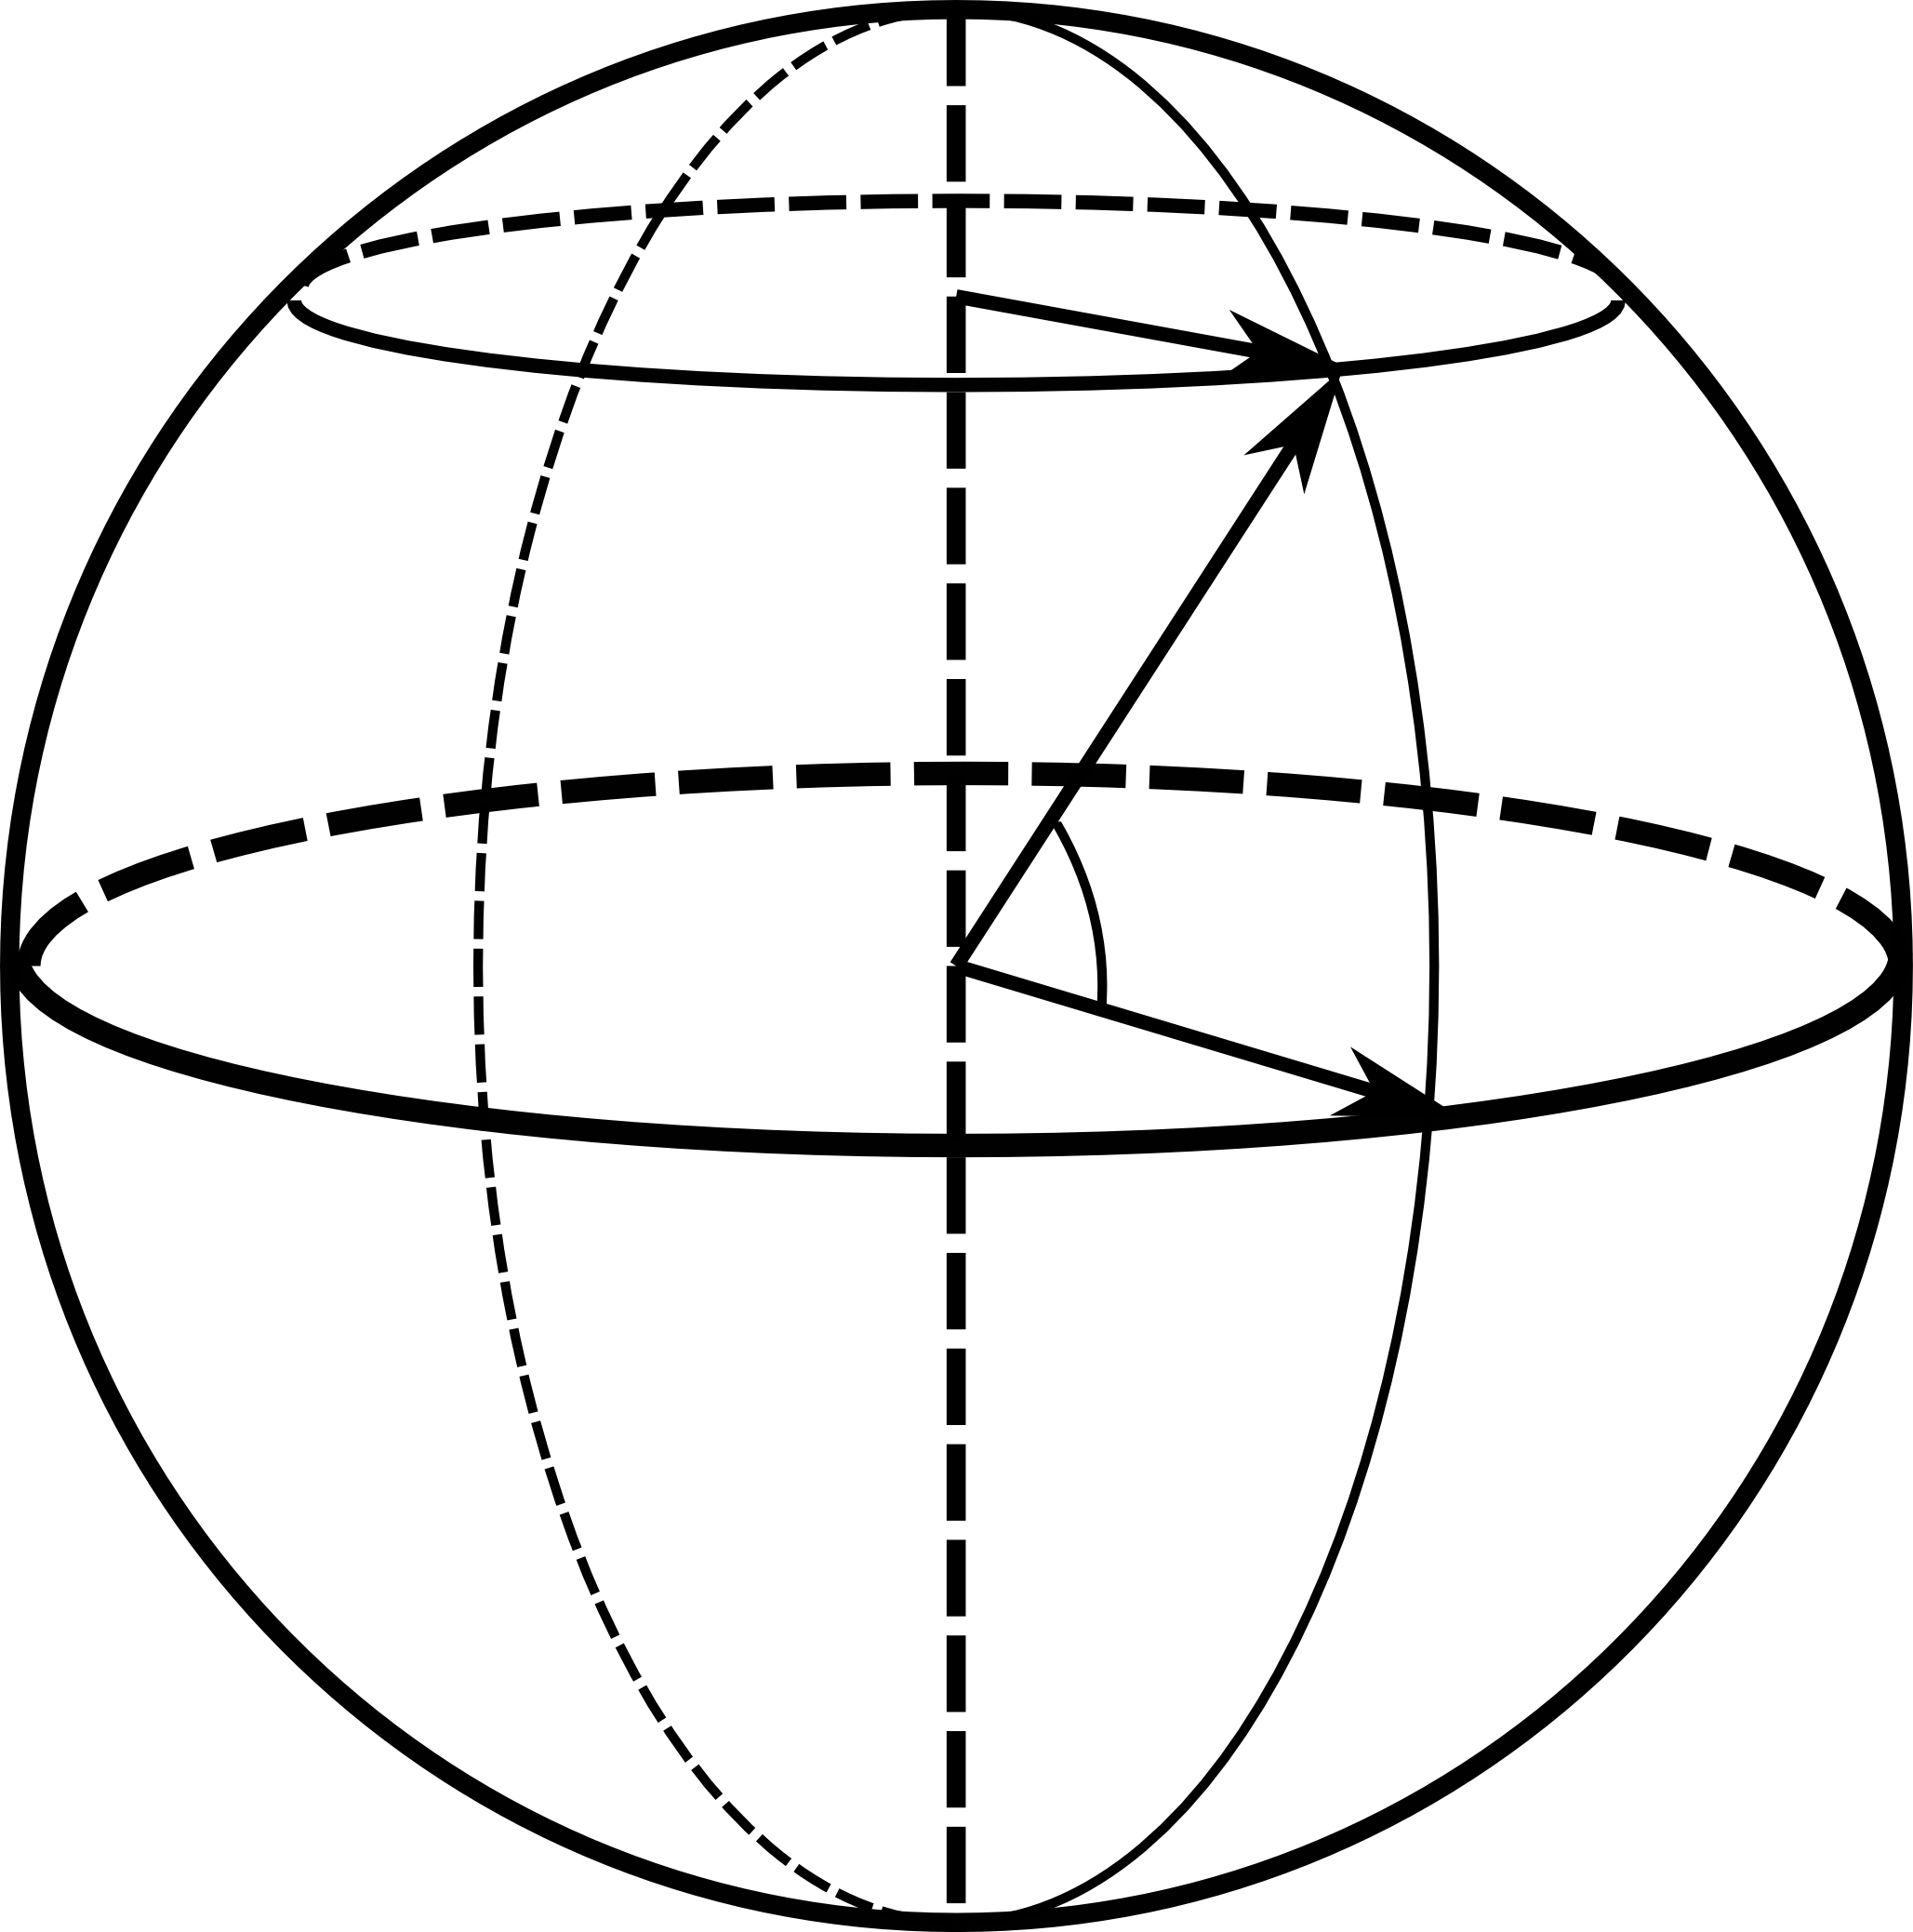
\includegraphics[scale=1.0]{aardehoeksnelheid}}
\put(10,0){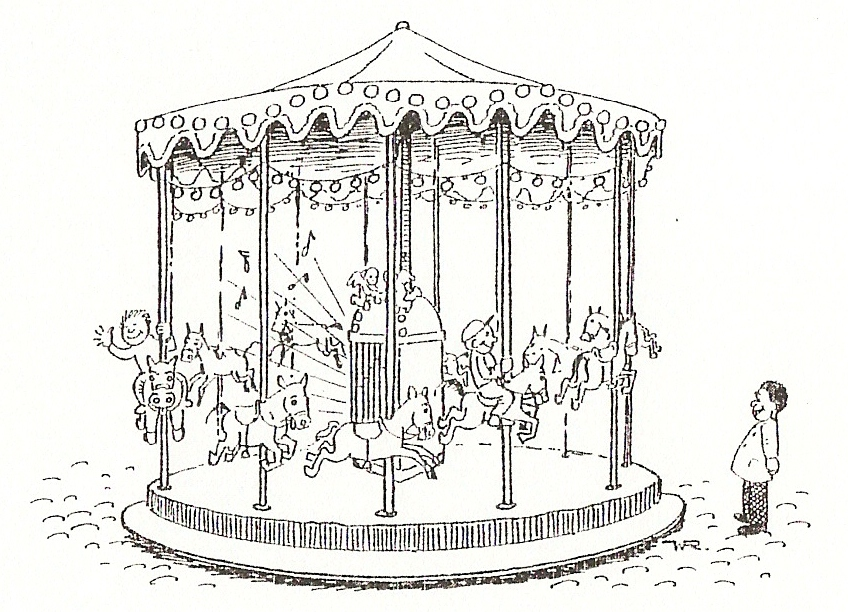
\includegraphics[width=90mm]{carrousel_trillingen}}
%\put(45,100){\textsc{DEEL II}}
\end{picture}
\end{center}

%\clearpage
%\newpage

%!TEX root = ../cursustekst_fys6.tex

\chapter*{Inleiding}

Er zijn legio voorbeelden waarin trillingen en golven voorkomen. Als inleiding zullen we er hier een niet onaardige kort aanstippen. Aanschouw de volgende wonderbaarlijke vergelijkingen \ldots
\begin{eqnarray*}
\vec{\nabla}\cdot\vec{E}&=&\frac{\rho}{\epsilon_0}\\[3mm]
\vec{\nabla}\times\vec{E}&=&-\frac{\partial\vec{B}}{\partial t}\\[3mm]
\vec{\nabla}\cdot\vec{B}&=&0\\[3mm]
c^2\vec{\nabla}\times\vec{B}&=&\frac{\vec{j}}{\epsilon_0}+\frac{\partial\vec{E}}{\partial t}\\
\end{eqnarray*}
Je zal misschien zeggen dat ze je niets zeggen. Toch ken je alle vier de vergelijkingen op \'e\'en term na. Je bent waarschijnlijk gewoon niet vertrouwd met de symbolen en de compacte manier waarop ze zijn weergegeven.\footnote{Het symbool $\vec{\nabla}$ staat voor $\vec{\nabla}=\frac{\partial}{\partial x}\vec{e}_x+\frac{\partial}{\partial y}\vec{e}_y+\frac{\partial}{\partial z}\vec{e}_z$. Het is een operator. Ze wordt de nabla-operator genoemd. $\times$ staat voor het vectorproduct (de derde rechterhandregel ken je om de richting van de resulterende vector te bepalen) en $\cdot$ staat voor het scalair product.} De letters E en B zouden wel een \emph{lichtje} moeten doen branden; het gaat over elektrische en magnetische velden. De vergelijkingen vormen de fundamentele wetten van het elektromagnetisme en worden de wetten van Maxwell\footnote{James Clerk Maxwell (1831 - 1879)} genoemd.\footnote{De eerste wet is de wet van Coulomb, maar dan beschreven voor elektrische velden in plaats van met krachten. Het symbool $\rho$ staat hier niet voor massadichtheid maar voor ladingsdichtheid. De term $\vec{\nabla}\cdot\vec{E}$ wordt de divergentie van het elektrisch veld genoemd en beschrijft de mate waarin het veld in een punt in de ruimte wordt opgewekt. De wet geeft de relatie tussen een lading en het elektrisch veld dat ze genereert. $\epsilon_0$ is op $4\pi$ na gelijk aan de constante $k$ in de wet van coulomb: $k=\frac{1}{4\pi\epsilon_0}$.

De tweede wet is de elektromagnetische inductiewet. De term in het linkerlid wordt de rotor van het elektrisch veld genoemd. Ze meet in hoeverre het veld een vortex of draaibeweging vertoont. Het rechterlid geeft de verandering van het magnetisch veld aan. Er staat de afgeleide naar de tijd (de gekrulde delta $\partial$ kan je lezen als een $d$). Herinner je dat een bewegende magneet een stroom kan opwekken in een spoel. De stroom volgt een cirkel waarvan het vlak loodrecht op de bewegingsrichting van de magneet staat. 

De derde wet ken je ook. Ze zegt dat de divergentie van het magnetisch veld nul is. Met andere woorden kunnen er in een punt in de ruimte niet meer magnetische veldlijnen vertrekken dan dat er toekomen. Magnetische veldlijnen zijn gesloten of er zijn geen monopolen voor het magnetisme \ldots

Als we bij de vierde wet de tweede term in het rechterlid even wegnemen, en lezen dat $\vec{j}$ voor de stroomsterkte staat, dan staat hier de wet die je in het 5de onder de vorm $B=\frac{\mu_0}{2\pi}\frac{I}{d}$ hebt geleerd. Het is de wet van Biot-Savart. Ze geeft de relatie tussen de stroomsterkte en de sterkte van het magnetisch veld dat rond de draad wordt gegenereerd. Herinner je dat de veldlijnen concentrische cirkels waren en zie dat het linkerlid nu de rotor van dat magnetisch veld is. Het linkerlid meet dus de mate waarin het magnetisch veld rondgaat.} \footnote{\textit{Ceci n'est pas une voetnoot.}\footnotemark}\footnotetext{In de strikte betekenis van het woord wel, maar dan toch een van ondergeschikt belang.}

Dit is niet omdat hij ze heeft uitgevonden maar omdat hij -- naast die ene term die je niet kent er aan toegevoegd te hebben -- de verschillende bestaande wetten heeft samengevoegd. Zo eenvoudige, compacte vergelijkingen met symbolen die een lust zijn voor het oog, in een wiskundige taal die onze snaar van zuivere logica en abstractie doet trillen, omvatten en beschrijven een onwaarschijnlijke uitgebreide waaier van verschijnselen. Dat is fysica ten top!

In de vergelijkingen staat ook een $c$\ldots Juist ja, de $c$ van de lichtsnelheid. Op het eind van de 19de eeuw was er bij het opstellen van de vergelijkingen nog geen $c$ aanwezig. In de plaats van $c^2$ stond er $\frac{1}{\mu_0\epsilon_0}$ oftewel\footnote{Door $c$ in de vierde vergelijking te vervangen en de laatste term in het rechterlid weg te laten, herken je enigszins de jouw bekende formule $B=\frac{\mu_0}{2\pi}\frac{I}{d}$. De uitdrukking $2\pi d$ als omtrek van een cirkel zit vervat in $\vec{\nabla}\times\vec{B}$.}
\begin{equation}
	c=\frac{1}{\sqrt{\mu_0\epsilon_0}}.
\end{equation}
Maxwell kende echter de waarde van $c$ en zag de gelijkenis\ldots. Bovendien liet hij zien dat een golvend elektrisch en een golvend magnetisch veld dat zich met dezelfde waarde als de lichtsnelheid voortplantte, een oplossing was van de vergelijkingen\footnote{Deze voetnoot bekijk je beter wanneer we het hoofdstuk over golven achter de rug hebben. En zelfs dan is hij niet zomaar te verstaan\ldots Maar we lopen hier toch even voor op de feiten. In het luchtledige reduceert de eerste vergelijking tot $\vec{\nabla}\cdot\vec{E}=0$ en de laatste tot $c^2\vec{\nabla}\times\vec{B}=\frac{\partial\vec{E}}{\partial t}$. Er zijn dan immers geen ladingen en geen stromen. Net iets geavanceerder rekenen met $\vec{\nabla}$ levert, als we slechts \'e\'en dimensie beschouwen, de vergelijking $\frac{\partial^2E}{\partial t^2}=c^2\frac{\partial^2E}{\partial x^2}$ op. Dit is een golfvergelijking met $E=E_0\sin(kx -\omega t)$ als mogelijke oplossing als $c=\lambda f$. Dit kan je nagaan door in te vullen. De oplossing is dus een golf die zich met de lichtsnelheid voortbeweegt!}. Dat wilde zeggen dat hij dus een tot dan toe onverklaarbaar verschijnsel als het licht kon verklaren met een elektromagnetische golf. En dit als \emph{gevolg} van de opgestelde wetten. Om het in zijn eigen woorden te zeggen:
\begin{quotation}
\emph{This velocity is so nearly that of light, that it seems we have strong reasons to conclude that light itself [\ldots] is an electromagnetic disturbance in the form of waves propagated through the electromagnetic field according to electromagnetic laws.}
\end{quotation}
Het ongelofelijk knappe hiervan is dat die wetten hun oorsprong vinden in verschijnselen die daar op het eerste zicht niets mee te maken hebben: het aantrekken en afstoten van ladingen, magneten en stromen. Deze verschijnselen zijn in de eeuwen daarvoor onderzocht en door verschillende grote fysici in wetmatigheden gegoten om vervolgens, als bijkomende consequenties, ook licht, radiogolven, gsm-straling en alle andere golven binnen het elektromagnetische spectrum te kunnen beschrijven. Dat is binnen de fysica alweer een staaltje van unificatie!
%\newline
%\newline
%Zo zien we dat golven fundamentele natuurverschijnselen zijn. De moeite om te bestuderen dus\ldots 
%\newline
%\newline
%- E induceert B en omgekeerd
%- nabla uitschrijven

\newpage

\chapter{Harmonische trillingen}

Om golven te kunnen beschrijven, behandelen we eerst trillingen. Dat is een iets eenvoudiger verschijnsel. Trillingen zijn heen en weer gaande bewegingen op een lijn. Zo trilt bijvoorbeeld een gitaarsnaar wanneer je hem aanslaat, trilt het rietje in een hobo bij het blazen of trillen elektronen in de antenne van je gsm.


% \section{Enkele voorbeelden}
% 
% - geluid
% - licht
% - ht is sinus

\section{De harmonische oscillator}

Als eerste voorbeeld behandelen we een eenvoudig mechanisch systeem: een massa die aan een veer is bevestigd. We noemen dit een massa-veersysteem. En zoals we al zo vaak hebben gedaan, beschouwen we een model waar geen wrijving aanwezig is. Laten we bovendien de veer een horizontale ori\"entatie geven zodat we ook de zwaartekracht buiten beschouwing kunnen laten.
\begin{figure}[h]
\centering
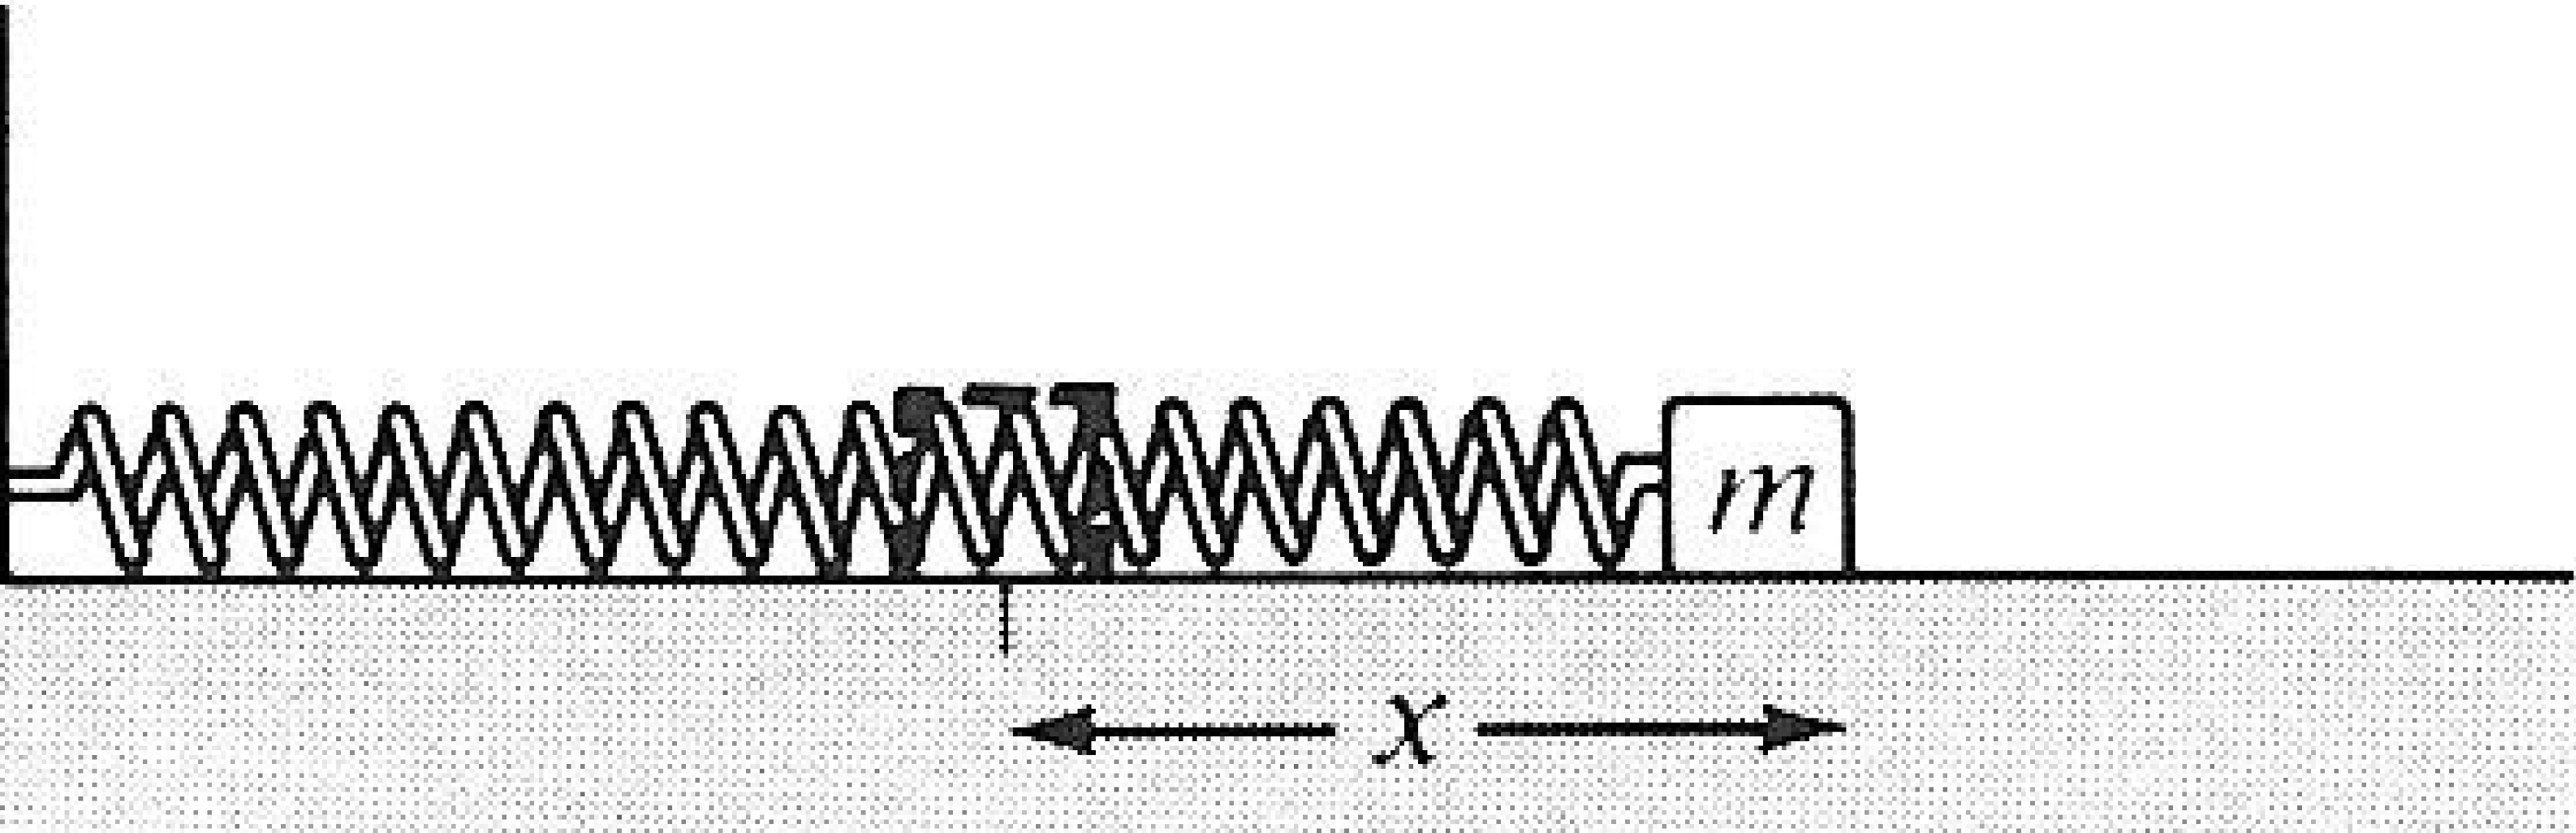
\includegraphics[width=0.8\textwidth]{kogeltegenveer2}
\end{figure}
Wanneer we de massa uit de positie halen waar de veer zijn rustlengte heeft en hem vervolgens loslaten, voert de massa een trilling uit. We constateren dat hij heen en weer beweegt waarbij hij steeds door de evenwichtspositie gaat. Deze beweging willen we natuurlijk uit onze natuurwetten tevoorschijn zien komen. Meer bepaald moet de tweede wet van Newton -- ons beginsel der beginselen in de klassieke mechanica -- de beweging opleveren. De trilling is een mechanisch verschijnsel en moet dus te verklaren zijn met behulp van die natuurwetten. 

Om de beweging te kunnen vinden, moeten we het systeem vrij maken -- alle krachten erop tekenen. We hebben dus de resulterende kracht nodig. Omdat het lichaam op een ondergrond rust en geen verticale versnelling heeft, heffen de normaalkracht en de zwaartekracht elkaar op. De resulterende kracht is bijgevolg de veerkracht. We gebruiken de wet van Hooke en gieten de component van de kracht volgens de bewegingsrichting in de vorm zoals we ze al kennen:\footnote{Deze beschrijving van de veerkracht is natuurlijk een benadering. Ze is maar geldig voor zolang de veer een niet te grote uitwijking kent. Het minteken zorgt voor een terugroepkracht; wanneer de co\"ordinaat $x$ positief is, is de component van de kracht negatief en wanneer de co\"ordinaat negatief is, is de component positief.}
\begin{eqnarray*}
F(x)=-kx
\end{eqnarray*}
Nu dat we ons model voor het massa-veersysteem hebben, kunnen we opzoek naar de beweging die de massa uitvoert. Hoe ziet de trilling er precies uit? De tweede wet van Newton dus \ldots
\begin{eqnarray}
F&=&ma\nonumber\\
&\Downarrow&\nonumber\\
-kx&=&m\frac{d^2x}{dt^2}\nonumber\\
&\Updownarrow&\nonumber\\
\frac{d^2x}{dt^2}+\frac{k}{m}x&=&0\label{diffvgl_ht}
\end{eqnarray}
\ldots\,en toen kwamen we uit bij een \ldots\,\emph{differentiaalvergelijking}. Om meer precies te zijn: een tweede-orde lineaire differentiaalvergelijking met constante co\"effici\"enten. Dat klinkt redelijk ingewikkeld. In feite is het ook niet zo simpel. We zijn opzoek naar de beweging, wat betekent dat we de positie $x$ in functie van de tijd willen vinden -- de functie $x(t)$ dus. De vergelijking die we gevonden hebben is niet zozeer een algebra\"ische vergelijking in een onbekende variabele $x$ (zoals bijvoorbeeld een tweedegraadsvergelijking) dan wel \emph{een vergelijking voor een functie}!\footnote{Wanneer we de impliciete afhankelijkheid van de tijd expliciet aangeven,ziet de vergelijking er als volgt uit
\begin{eqnarray*}
\frac{d^2x(t)}{dt^2}+\frac{k}{m}x(t)=0
\end{eqnarray*}} We zoeken dus een functie die aan de vergelijking voldoet. Een functie die voldoet is dan een oplossing van de vergelijking en dus een mogelijke beweging die de massa kan volgen. We spreken hier in eerste instantie over \emph{een} oplossing omdat er a priori\footnote{Vooraf beschouwd. Zonder het gezien, ervaren of onderzocht te hebben.} verschillende oplossingen kunnen zijn.

Het oplossen van differentiaalvergelijkingen is bijna een stiel op zich. Want dergelijke vergelijkingen zijn er in alle maten, geuren, kleuren en vooral moeilijkheidsgraden. En aangezien we die cursus willen overlaten aan degene die zich bij verdere studies hierin wil verdiepen, hebben wij op dit moment geen directe manier om tot de oplossingen te komen. Dat betekent dat we hier iets creatiever zullen moeten zijn en de methode van het ge\"inspireerd gokken zullen moeten toepassen \ldots In de modus van minder hoge ambities, kunnen we in eerste instantie een functie uit onze hoed toveren en nagaan of ze een oplossing is. Dat is natuurlijk onbegonnen werk wanneer we \'alle functies nagaan\footnote{Zoals het ook voor een schaakcomputer onbegonnen werk zou zijn, moest hij alle mogelijke zetten evalueren om de beste er uit te kunnen pikken.} maar haalbaar wanneer we ons fysisch inzicht erbij halen\footnote{Zoals ook een schaker alleen maar die paar zetten bestudeert waarvan hij ziet dat ze de moeite waard zijn.}. Zo moet de functie de beweging beschrijven en zullen de vergelijkingen voor een EVRB naar alle waarschijnlijkheid niet voldoen. De massa gaat heen en weer zodat we met een functie te maken moeten hebben die dat ook doet. Waarom zou dus een \emph{sinusfunctie} niet voldoen \ldots?!
\begin{figure}[h]
\centering
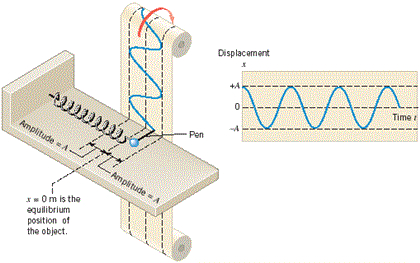
\includegraphics[width=.6\textwidth]{ht_papierrol}
\end{figure}

Om te proberen nemen we een eenvoudige sinusfunctie $x(t)=\sin\omega t$. Bij het invullen in de vergelijking (\ref{diffvgl_ht}) moeten we voor de eerste term in het linkerlid de tweede afgeleide berekenen; $x''(t)=-\omega^2\sin\omega t$. De tweede term geeft bij het invullen $\frac{k}{m}\sin\omega t$. Wil nu de voorgestelde functie een oplossing zijn, dan moet hetgeen we verkregen hebben, gelijk zijn aan het rechterlid -- namelijk nul.
\begin{eqnarray*}
 -\omega^2\sin\omega t+\frac{k}{m}\sin\omega t=0\Leftrightarrow\left(-\omega^2+\frac{k}{m}\right)\sin\omega t=0\Leftrightarrow\omega^2=\frac{k}{m}
\end{eqnarray*}
In de laatste overgang hebben we gebruik gemaakt van het feit dat de sinus welliswaar nul kan worden maar dit nooit voor \'alle tijdstippen het geval is. De vergelijking moet altijd opgaan -- niet enkel voor een paar momenten in de tijd. Wanneer we dus $\omega=\sqrt{k/m}$ nemen, is de voorgestelde functie een oplossing van de differentiaalvergelijking. We hebben zowaar een mogelijke beweging gevonden die de massa kan uitvoeren!

Natuurlijk hebben we nu slechts \emph{een} oplossing. Misschien zijn er nog. Want, waarom zou een cosinusfunctie niet voldoen? Een cosinusfunctie kunnen we beschrijven als een verschoven sinusfunctie zodat een sinusfunctie in algemene vorm $x(t)=a\sin(b(t-c))+d$ het proberen waard is. We kiezen voor het gemak $d$ gelijk aan nul\footnote{Dit komt overeen met het plaatsen van de oorsprong in de evenwichtspositie van de massa.} en geven in deze context de andere parameters andere symbolen: $a$ vervangen we door $A$, $b$ door $\omega$ en $-bc$ door $\varphi$. Die parameters hebben nl. een iets meer fysische betekenis -- waarover later meer. Ga nu na\footnote{Doe dit effectief. En nee, al liggend in je bed en kijkend naar dit blad voldoet niet aan de imperatief. Iets nagaan in deze exacte wereld van wiskunde en natuurkunde doet men met pen en papier / bord en krijt. Eventueel bijgestaan door een computer.} dat de functie 
\begin{eqnarray*}
x(t)=A\sin(\omega t+\varphi)\quad\mathrm{met}\quad\omega=\sqrt{\frac{k}{m}}
\end{eqnarray*}
een oplossing is van de differentiaalvergelijking. In feite is dit de algemene oplossing van de differentiaalvergelijking. Hier hebben we de existentie aangetoond; het feit dat er een oplossing bestaat. De uniciteit ervan -- het feit dat er geen andere functie bestaat -- is nog een ander paar mouwen.

Samengevat vinden we dat voor een lineaire terugroepkracht $F=-kx$ de beweging een harmonische trilling is. Ook het omgekeerde is waar: voert een lichaam een harmonische trilling uit, dan is de kracht lineair en steeds naar de oorsprong gericht.
\begin{eqnarray}
\frac{d^2x}{dt^2}+\frac{k}{m}x&=&0\nonumber\\
&\Updownarrow&\nonumber\\
x(t)=A\sin(\omega t+\varphi)\quad&\mathrm{met}&\quad\omega=\sqrt{\frac{k}{m}}\label{opl_diffvgl_ht}
\end{eqnarray}
We hebben nu de wiskundige oplossing van de differentiaalvergelijking gevonden. De massa trilt sinuso\"idaal in de tijd. Vandaar dat we over een harmonische trilling spreken.

De verschillende parameters die in de oplossing (\ref{opl_diffvgl_ht}) voorkomen, willen we fysisch kunnen interpreteren. We willen hun betekenis kennen. Het gemakkelijkste is misschien terug te grijpen naar de algemene sinusfunctie. Daar stond de parameter $a$ voor de amplitude. Dat is dus hier voor $A$ niet anders; $A$ stelt de amplitude van de trilling voor. Voor de parameter $b$ hebben we de gelijkheid $b=\frac{2\pi}{p}$ waarin $p$ de periode van de functie is. Omdat onze onafhankelijke variabele de tijd is, is de fysische interpretatie van $p$ de tijd van \'e\'en cyclus -- waarvoor we het symbool $T$ gebruiken. 
\begin{figure}[h]
\centering
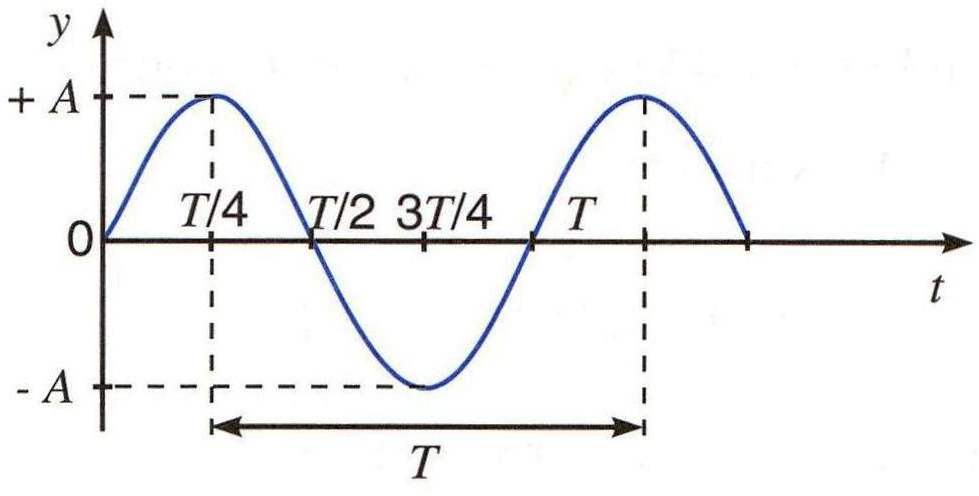
\includegraphics[width=.7\textwidth]{ht_tijd}
\end{figure}
Voor de parameter $\omega$, die we de pulsatie noemen, geldt dus
\begin{eqnarray*}
\omega=\frac{2\pi}{T}
\end{eqnarray*}
De pulsatie bepaalt dus de frequentie waarmee de massa trilt. Aangezien voor het massa-veersysteem geldt dat $\omega=\sqrt{k/m}$, kunnen we een uitdrukking voor periode en de frequentie vinden:
\begin{eqnarray*}
T=2\pi\sqrt{\frac{m}{k}},\quad f=\frac{1}{2\pi}\sqrt{\frac{k}{m}}
\end{eqnarray*}
De frequentie wordt bepaald door de sterkte van de veer en de grootte van de massa. Een grotere massa levert een kleinere frequentie op (de traagheid is groter) en een sterkere veer zorgt voor een grotere frequentie (de massa krijgt een grotere versnelling). De amplitude speelt blijkbaar geen rol.

De parameter $\varphi$ is iets lastiger om inzichtelijk te kunnen duiden. Net zoals de amplitude wordt ze bepaald door de \emph{beginvoorwaarden}. Zo is de amplitude afhankelijk van bijvoorbeeld de afstand uit de evenwichtspositie waarop we de massa vanuit rust loslaten of van de snelheid die we ze bij initiatie van de beweging meegeven. De parameter $\varphi$ wordt bepaald door de positie van de massa op het tijdstip $t=0$. Immers is $x_0=x(t=0)=A\sin(\varphi)$. Het argument van de sinus\footnote{Het argument van de sinus is hetgeen waarvan de sinus wordt genomen/hetgeen dat tussen haakjes staat.} $\omega t+\varphi$ noemen we ook wel de \emph{fase} van de trilling zodat $\varphi$ de \emph{beginfase} wordt genoemd. De fase drukken we natuurlijk uit in radialen. De fase bepaalt waar we ons in de cyclus bevinden. 
%\begin{figure}[h]
%\centering
%\includegraphics[width=.7\textwidth]{ht_fase}
%\end{figure}
%\newline
De beginfase bepaalt dan ook de beginpositie. Zo is bijvoorbeeld de functie maximaal wanneer het argument $\pi/2$ is, wat betekent dat de massa op haar maximale uitwijking is. Is dus de beginfase gelijk aan $\pi/2$, dan begint de trilling vanuit haar maximale uitwijking. Een beginfase van $3\pi/2$ komt overeen met een minimale waarde bij het begin. In figuur \ref{beginposbeginfase} zie je verschillende mogelijkheden voor de beginfase, hier weergegeven als $\varphi_0$.

Nu dat we de positie in functie van de tijd kennen, vinden we door af te leiden de snelheid en de versnelling van de massa. 
\begin{eqnarray*}
x&=&A\sin(\omega t+\varphi)\\[3mm]
v=\frac{dx}{dt}&=&\omega A\cos(\omega t+\varphi)\\[3mm]
a=\frac{d^2x}{dt^2}&=&-\omega^2A\sin(\omega t+\varphi)=-\omega^2x
\end{eqnarray*}
Merk op dat de versnelling op een constante ($\omega^2$) na tegengesteld is aan de positie. Dat is niet verwonderlijk aangezien we te maken hebben met de wet van Hooke en volgens de tweede wet van Newton de versnelling recht evenredig is met de kracht. 

\newpage

\begin{figure}
	\centering
	\includegraphics[width=.9\textwidth]{trillendeveer_a}
	\includegraphics[width=.9\textwidth]{trillendeveer_b}
	\includegraphics[width=.9\textwidth]{trillendeveer_c}
	\includegraphics[width=.9\textwidth]{trillendeveer_d}
	\caption{Relatie tussen beginpositie en beginfase}
	\label{beginposbeginfase}
\end{figure}

\clearpage
\newpage

Naast in detail de beweging te hebben bestudeerd, kunnen we ook naar het energieverloop kijken. Hiertoe vullen we gewoonweg de positie en de snelheid in de formules voor energie in.
\begin{eqnarray*}
E_k&=&\frac{mv^2}{2}=\frac{1}{2}m\omega^2A^2\cos^2(\omega t+\varphi)\\
E_p&=&\frac{1}{2}kx^2=\frac{1}{2}kA^2\sin^2(\omega t+\varphi)=\frac{1}{2}m\omega^2A^2\sin^2(\omega t+\varphi)
\end{eqnarray*}
Deze hangen duidelijk af van de tijd. Wanneer we naar de totale energie kijken, vinden we -- zoals we volgens de wet van behoud van energie mogen verwachten -- dat deze constant is.
\begin{eqnarray*}
E=E_k+E_p=\frac{1}{2}m\omega^2A^2\left(\sin^2(\omega t+\varphi)+\cos^2(\omega t+\varphi)\right)=\frac{1}{2}m\omega^2A^2
\end{eqnarray*}
\begin{figure}[h]
\centering
%\includegraphics[width=.7\textwidth]{EpEkE}
\includegraphics[width=.9\textwidth]{ht_behoud_energie}
\end{figure}
Merk op dat de energie van een trilling recht evenredig is met het kwadraat van de amplitude. Een golf in de zee die dus twee keer zo hoog is, draagt vier keer zoveel energie met zich mee. In de figuur zie je mooi hoe de kinetische en de potenti\"ele energie in elkaar worden omgezet; het verlies van de ene is de winst van de andere. Let op het verschil tussen de periode van de energievormen en de periode van de eigenlijke trilling \ldots

%\newpage

\section{Relatie met een cirkelbeweging}

Wanneer we op een grammofoonplaat en klein object leggen en met een lamp de schaduw op de muur bekijken terwijl de plaat draait, dan zien we evenzeer een op- en neergaande beweging. 
\begin{figure}[h]
%\centering
\includegraphics[width=.6\textwidth]{ht_schaduw}
\hspace{5mm}
\includegraphics[width=.35\textwidth]{fasor}
\end{figure}
Het gaat hier echter ook om een harmonische trilling. Bekijken we immers de $y$-co\"ordinaat van een punt op een cirkel dat met een constante hoeksnelheid beweegt, dan is dit een sinusfunctie. Als we bovendien de hoeksnelheid van de cirkelbeweging gelijk nemen aan de pulsatie van een harmonische trilling, de straal even lang maken als de amplitude en op tijdstip $t=0$ het punt op de cirkel een omwentelingshoek $\varphi$ geven, dan beschrijft de $y$-co\"ordinaat eenzelfde harmonische trilling. 

De plaatsvector die het punt op de cirkel beschrijft noemen we ook wel een \emph{fasor} -- een samenvoegsel van fase en vector. Met een fasor kunnen de fase van een trilling visualiseren, het faseverschil tussen trillingen visualiseren en kunnen we gemakkelijker trillingen samenstellen. 

%\newpage

\section{De mathematische slinger}

Als tweede voorbeeld bekijken we een massa aan een touw. Geen erg spectaculair systeem, zal je denken. Toch zal je snel zien dat de beweging verre van eenvoudig is.

Stel dat we te maken hebben met een slinger van lengte $l$ die bovenaan bevestigd is en waaraan een massa $m$ hangt. De wrijving laten we buiten beschouwing. We beschouwen ook een model waarin het touw geen massa heeft.\footnote{Moesten we dit wel in rekening brengen, dan zouden we het model de fysische slinger noemen.} De positie van de slinger kunnen we aangeven d.m.v. de booglengte, gemeten vanaf de evenwichtspositie tot aan de massa. De hoek die het touw met de verticale maakt, is een mogelijk alternatief. 

Om de beweging te kunnen vinden d.m.v. de tweede wet van Newton, maken we een krachtendiagram. We voeren een assenstelsel rakend aan de baan van het voorwerp in. De richting rakend aan de baan noemen de tangenti\"ele richting, die loodrecht op de baan noemen we de normale richting. Natuurlijk kunnen we ook altijd voor een $x$-as en een $y$-as opteren.
\newline
\begin{wrapfigure}[11]{r}{0.33\textwidth}
%\centering
\includegraphics[width=0.34\textwidth]{pendulum}
%\caption{A gull}
\end{wrapfigure}
Volgens de normale richting zal de spankracht in het touw in combinatie met de normale component van de zwaartekracht voor de nodige middelpuntzoekende kracht zorgen. De massa beweegt immers op een cirkel met vari\"erende snelheid waardoor ook een vari\"erende middelpuntzoekende kracht nodig is. Echter kunnen we volgens deze richting niet veel leren over de manier waarop de massa heen en weer slingert. Daarvoor hoeven we enkel de tangenti\"ele richting te bekijken. We passen dan ook de tweede wet van Newton volgens deze richting toe. 
\begin{gather*}
F=ma\\
\Downarrow\\
-mg\sin\theta=m\frac{d^2s}{dt^2}\\
\phantom{\theta=\frac{s}{l}}\Updownarrow\theta=\frac{s}{l}\\
\frac{d^2s}{dt^2}+g\sin\left(\frac{s}{l}\right)=0
\end{gather*}
Dit is een \emph{niet}-lineaire differentiaalvergelijking. Ze is verre van eenvoudig om exact op te lossen. We hebben daartoe een veel zwaarder arsenaal aan wiskundige functies nodig dan dat wij op dit moment kennen. In feite is dat ook niet zo verwonderlijk. Wanneer we bijvoorbeeld de slinger vanuit een initi\"ele hoek van 120 graden met een voldoende hoge beginsnelheid laten vertrekken, zal de slinger niet slingeren maar pulserende rondjes blijven draaien. Deze oplossing samen met bijvoorbeeld stil blijven hangen op 180 graden en nog andere varianten, zijn allemaal mogelijkheden die aan de differentiaalvergelijking moeten voldoen. Ingewikkeld dus.

Wij zullen ons hier beperken tot kleine hoeken\footnote{Ik weet het, dat doet pijn aan het wiskundig exacte deel van ons hart, maar in feite is het in de fysica nooit anders \ldots \'Alles wat we in de fysica doen is een benadering van de realiteit. Zo hebben we bij onze slinger reeds de massa van het touw overboord gegooid, de massa van het object geen dimensie gegeven, gedaan alsof de wrijvingskracht niet bestaat, de zwaartekracht benaderd door $mg$ terwijl die eigenlijk afhankelijk is van de hoogte boven het aardoppervlak, de wetten van Newton gebruikt waar we eigenlijk de wetten van de kwantummechanica zouden moeten bovenhalen, gedaan alsof slingers het enige in het universum zijn \ldots }. In dat geval kunnen we de sinus van een argument benaderen door het argument zelf, $\sin\alpha\approx\alpha$. \footnote{Herinner je misschien dat je ooit de limiet $\displaystyle\lim_{x\rightarrow0}\frac{\sin x}{x}=1$ bewezen hebt.} \footnote{In feite is de wet van Hooke enzelfde lineaire benadering van de veerkracht. Die is ook maar geldig voor zolang we de veer niet te ver uitrekken. Willen we accurater zijn, dan moeten we termen afhankelijk van bijvoorbeeld $x^2$ in rekening brengen \ldots}
\begin{figure}[h]
\centering
\includegraphics[width=0.4\textwidth]{sinx_x}
\end{figure}
% \begin{minipage}[t]{.5\textwidth}
% \begin{eqnarray*}
% \sin\alpha\approx\alpha
% \end{eqnarray*}
% \end{minipage}
% \begin{minipage}[t]{.4\textwidth}
% \phantom{}
% \includegraphics[width=\textwidth]{sinx_x}
% \end{minipage}
\newline
De differentiaalvergelijking wordt er dan een heel pak gemakkelijker op:
\begin{eqnarray*}
\frac{d^2s}{dt^2}+g\sin\left(\frac{s}{l}\right)&=&0\\
&\rotatebox[origin=c]{-90}{$\rightsquigarrow$}&\mathrm{benadering} \sin\alpha\approx\alpha\\
\frac{d^2s}{dt^2}+\frac{g}{l}s&=&0
\end{eqnarray*}
We vinden zo niets anders dan de differentiaalvergelijking van de harmonische trilling (\ref{diffvgl_ht}). De oplossing is wiskundig gezien dan ook dezelfde\footnote{Zo zie je maar hoe we een eenheid in verschillende verschijnselen kunnen terugvinden.}.
\begin{gather*}
\frac{d^2s}{dt^2}+\frac{g}{l}s=0\quad\Leftrightarrow\\
%\Updownarrow\\
s(t)=A\sin(\omega t+\varphi)\quad\mathrm{met}\quad\omega=\sqrt{\frac{g}{l}}
\end{gather*}
Realiseer je dat de amplitude hier de booglengte bij maximale uitwijking is. Ook zien we dat de slingerlengte de periode van de trilling bepaalt en dat de amplitude noch de massa hierop een invloed heeft \ldots
\begin{eqnarray*}
T=2\pi\sqrt{\frac{l}{g}},\quad f=\frac{1}{2\pi}\sqrt{\frac{g}{l}}
\end{eqnarray*}

\newpage

\section{Resonantie}

% microgolfoven

Het verschijnsel resonantie is je zeker bekend. Naar alle waarschijnlijkheid heb je ooit je kleine zusje geduwd op de schommel. Uiteraard deed je dat niet zomaar willekeurig maar met de juiste regelmaat. Je duwde wanneer ze net voorbij het hoogste punt bij jou was -- niet wanneer ze naar je toe kwam! Op die manier ging zij hoger en hoger en nam het plezier alleen maar toe. En dat totdat ze schrik kreeg omdat jij te ver ging \ldots

We beschouwen een model waarin we een massa-veersysteem niet langer vrij laten trillen maar onderwerpen aan een periodieke aandrijvende kracht waarvan we de frequentie controleren. We hebben dan een gedwongen trilling. In ons model kunnen we natuurlijk allerlei soorten manieren van externe krachten steken maar om een differentiaalvergelijking te bekomen die toch ergens hanteerbaar is, nemen we een oscillerende kracht $F=F_0\cos\omega t$ waarin $F_0$ de maximale kracht is waarmee we trekken of duwen en $\omega$ de pulsatie waarmee we de kracht sinuso\"idaal laten vari\"eren. Ook voegen we ditmaal wrijving toe. We nemen een model waarin de wrijvingskracht recht evenredig is met snelheid $F_w=-cv$. Hierin is $c$ een co\"effici\"ent die de sterkte van de demping bepaalt. Het minteken zorgt ervoor dat de component van de wrijvingskracht steeds tegengesteld is aan de snelheid; de wrijvingskracht werkt de beweging altijd tegen. Zolang de snelheid niet te groot wordt, is dit een realistisch model. We vertrekken weer met de tweede wet van Newton:
\begin{gather}
F=ma\nonumber\\
\Downarrow\nonumber\\
-kx-cv+F_0\cos\omega t=ma\nonumber\\
\Updownarrow\nonumber\\
x''+\gamma x'+\omega_0^2x=\frac{F_0}{m}\cos\omega t\label{diffvgl_resonantie}
\end{gather}
Waarin we $c/m$ hebben vervangen door een nieuw symbool $\gamma=c/m$ en ook $\omega_0$ hebben gebruikt voor $\sqrt{k/m}$. $\omega_0=\sqrt{k/m}$ is de natuurlijke pulsatie; de frequentie (op $2\pi$ na) waarmee de massa zou trillen, moest ze vrij worden gelaten.

De oplossing\footnote{Het oplossen van deze vergelijking is relatief eenvoudig wanneer we complexe e-machten gebruiken.\footnotemark Alleen kennen we die nog niet omdat ze alweer gereserveerd zijn voor een vervolgstudie na het 6de. Er moet nog \'iets overblijven om te bestuderen na je humaniora.}\footnotetext{Eenvoudig - complex: heb je'm?} van deze differentiaalvergelijking die overblijft na een zekere tijd wordt gegeven door
\begin{eqnarray*}
x(t)=A\cos(\omega t-\varphi)&\mathrm{met}&
\begin{array}[t]{rcl}
\displaystyle A&=&\frac{F_0/m}{\sqrt{(\omega_0^2-\omega^2)^2+\gamma^2\omega^2}}\\
\displaystyle\tan\varphi&=&\frac{\gamma\omega}{\omega_0^2-\omega^2}
\end{array}
\end{eqnarray*}
Dat betekent dat de massa, na een korte overgangsperiode of nadat de eerste onregelmatige trillingen zijn uitgedoofd, een harmonische trilling zal uitvoeren met dezelfde frequentie als de externe aandrijving. Het bijzondere is echter terug te vinden in de amplitude. We zien dat al naargelang de opgelegde frequentie, we een andere amplitude krijgen. En jawel, als we een grafiek maken van de amplitude in functie van de aandrijving $\omega$ zien we dat in de buurt van de natuurlijke frequentie $\omega_0$ (om precies te zijn, een waarde die net iets kleiner is) de amplitude een sterke piek vertoont. 
\begin{figure}[h]
\centering
\includegraphics[width=.55\textwidth]{resonantie_curve}
\caption{$A$ in functie van $\omega$.}
\end{figure}
De frequentie waarbij dit optreedt noemen we de \emph{resonantiefrequentie}. Het systeem zal dus bij \'e\'en specifieke frequentie extreem meetrillen. Op de juiste momenten wordt er dus aan de massa geduwd/getrokken zodat er maximaal energie wordt `ingepompt'. Die energie gaat dan natuurlijk weer verloren door de demping.

%Uit de afhankelijkheid van het faseverschil $\varphi$ van de trilling t.o.v. de extern aangelegde trilling, valt op te maken dat bij de resonantiefrequentie het faseverschil $\pi/2$ is; de trilling ijlt een kwart cyclus na op de aandrijving. Naarmate de externe frequentie groter en groter wordt, gaat de massa meer en meer in tegenfase trillen. Het faseverschil nadert $\pi$.
%\begin{figure}[h]
%\centering
%\includegraphics[width=.55\textwidth]{resonantie_fase}
%\caption{$\varphi$ in functie van $\omega$.}
%\end{figure}

%\section{Samenstellen van trillingen}
%- Fourieranalyse?

%\cleardoublepage
%!TEX root = ../fys_cursus.tex

%\the\textwidth
% 390 pt = 13.7323943 cm (1pt=28,4 cm)

\chapter{Golven}

Als je een steentje in een poel gooit, krijg je van die prachtige uitdijende cirkels in het wateroppervlak, die, al naargelang ze groter worden, ook in zichtbaarheid afnemen en meer en meer verdwijnen. De verstoring die door de steen in het wateroppervlak teweeg is gebracht, plant zich voort in het water. We hebben te maken met een golf.
\newline
Een bijzondere eigenschap van de golf die in het wateroppervlak ontstaat is dat het de verstoring in het medium is die zich verplaatst, niet het water zelf. Het water blijft ter plaatse. Zo zal een dobber van een vislijn enkel op en neer bewegen wanneer een golf voorbijkomt. Ook bij een Mexican wave is dit duidelijk; het zijn niet de supporters die rondlopen!
\newline
Golven hebben echter niet altijd een medium nodig om zich in voort te planten. Denk maar aan licht of in het algemeen aan een elektromagnetische golf. De wisselende elektrische en magnetische velden vormen hier de golf.

%een golf heeft een trilling als bron. Als de bron een harmonische trilling uitvoert, ontstaat een golf die zowel in de ruimte als in de tijd sinuso\"idaal is.

%golf = def

\section{Golven \& kenmerken}

Golven kunnen we volgens hun kenmerken indelen in een paar categori\"en. Zo kunnen we een onderscheid maken tussen \emph{mechanische} en \emph{elektromagnetische} golven. Mechanische golven hebben een (elastisch\footnote{De vervorming in het medium kan zich maar voortzetten van zodra het lichaam te vervormen is en dus elastisch is. Er moeten immers krachten tussen de verschillende plaatsen van het medium aanwezig zijn.}) medium nodig om zich in te verplaatsen -- het is de storing in het medium die de golf vormt. Elektromagnetische golven daarentegen hebben geen medium nodig. Het zijn de elektrische en de magnetische veldenvectoren die golven.\footnote{Ook de recentelijk gemeten zwaartekrachtgolven moeten tot de categorie behoren van golven die geen medium nodig hebben. Het zijn rimpelingen van de ruimte-tijd zelf.}
\begin{figure}[h]
\centering
\includegraphics[width=0.7\textwidth]{elasticiteit_medium}
\caption{\textit{Een golfpuls die zich voortplant in een touw. De pijlen geven de snelheid van deeltjes in het touw weer.}}
\end{figure}
\newline
\newline
Golven kunnen \emph{transversaal} of \emph{longitudinaal} zijn. Bij een transversale golf gebeurt de beweging van de deeltjes van het medium loodrecht op de voortplantingsrichting van de golf. Zo krijg je transversale golven wanneer je het uiteinde van een touw heen en weer slingert. Ook licht is een transversale golf. Hier trilt dus niet het medium maar is het de ori\"entatie van de elektrische of magnetische veldvector die loodrecht staat op de voortplantingsrichting. Bij een longitudinale golf bewegen de deeltjes van het medium in de richting evenwijdig met de voortplantingsrichting. P-golven bij een aardbeving zijn hiervan een voorbeeld (i.t.t. S-golven, die zijn transversaal). Ook geluid bestaat uit een longitudinale golf. Zo plant geluid zich in de lucht voort doordat de luchtmoleculen tegen elkaar botsen. 
Er zijn nog andere soorten golven zoals \emph{oppervlaktegolven}, \emph{tweedimensionale} en \emph{driedimensionale} golven. Deze zullen we hier met momenten kort behandelen.
\begin{figure}[h]
\centering
\includegraphics[width=0.9\textwidth]{longitudinaal_veer}
\caption{\textit{Een longitudinale golf in een opgegespannen veer. De verplaatsingen van de spiralen zijn in de richting van de zich voortplantende golf. Elke samendrukking wordt gevolgd door een uitrekking.}}
\end{figure}
\newline
\newline
Als een de bron van een golf voortdurend blijft trillen, spreken we van een \emph{continue golf} of lopende golf. Als je slechts een enkele verstoring hebt die zich voortplant, spreken we van een \emph{puls}. We zullen hier in de regel over continue golven spreken.
\newline
\newline
Om een golf te kunnen beschrijven, hebben we een paar karakteristieke grootheden. Zo kunnen we bij een continue golf spreken over de \emph{golflengte}. De golflengte $\lambda$ van een golf is de kortste afstand tussen twee punten die in fase trillen. Deze is gemakkelijk terug te vinden als de afstand van top tot top\footnote{In de ruimtelijke voorstelling van de golf kan je over golftoppen, -pieken of -kammen spreken tegenover golfdalen. Voor een longitudinale golf spreken we over samendrukkingen of verdichtingen versus uitrekkingen of verdunningen.}. De golflengte is dus de periode voor de golf in de ruimte zoals de `periode' $T$ de periode is van een trilling in de tijd. Voor een continue golf is de \emph{periode} de tijd die een deeltje nodig heeft om een volledige trilling te doorlopen. Omdat dit evenzeer de tijd is die de storing nodig heeft om de golflengte af te leggen, hebben we de volgende eenvoudige maar belangrijke formule voor de snelheid waarmee de golf zich voortplant -- de \emph{golfsnelheid} of fasesnelheid:
\begin{equation*}
v=\frac{\lambda}{T}=\lambda\cdot f
\end{equation*}
%De eenheid van golflengte is dan ook de meter, daar waar die voor de periode de seconde is.
In de regel zullen we golven behandelen waarvoor de snelheid onafhankelijk is van de frequentie of golflente van de golf.\footnote{Is de snelheid wel afhankelijk van de frequentie, dan spreken we over dispersie. Dit verschijnsel doet zich onder andere voor bij licht dat door een prisma gaat. De snelheid voor verschillende kleuren en dus frequenties is verschillend waardoor je een regenboogeffect krijgt. De snelheid bepaalt immers de mate van breking.} In dat geval zijn golflengte en frequentie dus omgekeerd evenredig.
\newline
\newline
Voor een golf kan je naast de golfsnelheid nog een andere snelheid beschouwen. De deeltjes van het medium kunnen namelijk harmonisch trillen zodat hun snelheidsverloop helemaal verschillend is van de constante golfsnelheid waarmee de storing zich voortplant. De onderstaande figuur verduidelijkt dit.
\begin{figure}[h]
\centering
\includegraphics[width=0.9\textwidth]{golf_vs_deeltjessnelheid}
\caption{\textit{De golf beweegt naar rechts terwijl de deeltjes van het touw oscilleren.}}
\end{figure}

%- overdracht van energie

\section{Periodieke golven}

Zoals we de positie van een voorwerp konden beschrijven met een functie $x(t)$, willen we ook een golf m.b.v. een functie kunnen beschrijven. Omdat een golf niet te lokaliseren is in een punt maar zich uitstrekt over de hele ruimte en daarnaast in de tijd evolueert, hebben we een iets uitgebreidere functie nodig. De uitwijking $y$ van het medium is zowel afhankelijk van de plaats $x$ waarop je kijkt als het moment $t$ dat je interesseert. De oplossing bestaat erin een functie in twee variabelen te gebruiken. 
\newline
\newline
We beschouwen een sinuso\"idale golf die naar rechts beweegt -- volgens de $x$-as. Om een wiskundige beschrijving van een golf te vinden, bekijken we twee momentopnames op willekeurige tijdstippen. Voor het gemak nemen we als eerste tijdstip $t=0$ en noemen we het tweede tijdstip $t$. In de tijdsspanne $t$ is de golf $vt$ eenheden naar rechts opgeschoven, zie figuur (\ref{afleiding_golfvergelijking}). $v$ is uiteraard de golfsnelheid.

\begin{figure}[!h]
\centering

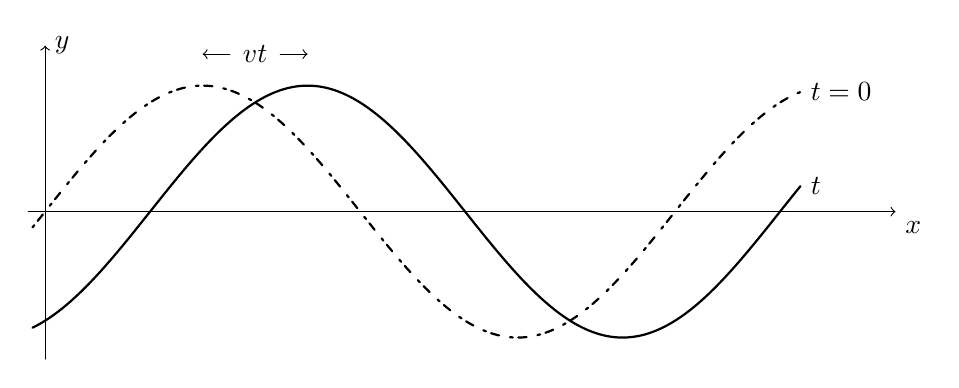
\begin{tikzpicture}[line cap=round,line join=round,x=8.0cm,y=8.0cm]
%\draw[very thin,color=gray] (0,-0.24) grid (1.4,0.24);
\draw[->,color=black] (-0.026820246306000255,0.) -- (1.35,0) node [anchor=north west] { $x$};
%\foreach \x in {0.1,0.2,0.3,0.4,0.5,0.6,0.7,0.8,0.9,1.,1.1,1.2,1.3,1.4}
%\draw[shift={(\x,0)},color=black] (0pt,2pt) -- (0pt,-2pt);
%\draw[color=black] (1.4,0) node [anchor=north west] { $x$};
\draw[->,color=black] (0.,-0.2341604564505571) -- (0.,0.2636169400770265) node [anchor=west] { $y$};
%\foreach \y in {-0.2,-0.1,0.1,0.2}
%\draw[shift={(0,\y)},color=black] (2pt,0pt) -- (-2pt,0pt);
%\draw[color=black] (0.008952830872798266,0.22422448423671415) node [anchor = south west] { $y$};
%\clip(-0.026820246306000255,-0.2341604564505571) rectangle (1.464721377102191,0.2636169400770265);
\draw[line width=0.8pt,dash pattern=on 1pt off 2pt on 3pt off 4pt,smooth,samples=100,domain=-0.02:1.2] plot(\x,{0.2*sin((6.283185307179586*(\x)-6.283185307179586)*180/pi)}) node[right] {$t=0$};
\draw[line width=0.8pt,smooth,samples=100,domain=-0.02:1.2] plot(\x,{0.2*sin((6.283185307179586*(\x)-6.283185307179586*(1.0+1/6))*180/pi)}) node[right] {$t$};
%\draw (0.03943070215270692,2.6289548566703287) node[anchor= north west] {$y$};
\draw[<-] (2/8,2/8) -- (2/8+1/12-0.04,2/8);
\draw[->] (2/8+1/12+0.04,2/8) -- (2/8+1/6,2/8);
\draw (1/3,2/8) node {$vt$};
\end{tikzpicture}

\caption{\emph{De uitwijking van een golf in functie van de tijd op $t=0$ en een willekeurig tijdstip $t$}}\label{afleiding_golfvergelijking}
\end{figure}

De verschijningsvorm van de golf in de ruimte kunnen we op $t=0$ weergeven met volgende sinusfunctie:
\begin{eqnarray*}
y=A\sin(kx)\qquad\mathrm{met}\qquad k=\frac{2\pi}{\lambda}
\end{eqnarray*}
Het symbool $k$ noemen we het \emph{golfgetal}.\footnote{De $k$ is eigenlijk niets anders dan de `$b$' zoals je die kent in de algemene sinusfunctie $f(x)=a\sin(b(x-c))$+d. $b=\frac{2\pi}{p}$ met $p$ de periode. In deze context is de periode de golflengte $\lambda$, uitgedrukt in meters.} \footnote{De $k$ heeft niets te maken met de veerconstante. Het is niet omdat Jantje Jantje heet en Jantje Jantje, dat Jantje en Jantje dezelfde personen zijn. Jantje en Jantje kunnen bijvoorbeeld -- al is het onwaarschijnlijk -- broers zijn.}
\newline
\newline
Een tijd $t$ later is de verschijningsvorm van de golf een afstand $vt$ (de afstand die een top gedurende de tijd $t$ heeft afgelegd) naar rechts opgeschoven. De vergelijking vinden we dan door een overeenkomstige verschuiving door te voeren:
\begin{eqnarray*}
y&=&A\sin(k(x-vt))\\
%&=&A\sin(kx-kvt)\\
&=&A\sin\left(kx-\frac{2\pi v}{\lambda}t\right)\\
&=&A\sin\left(kx-\frac{2\pi}{T}t\right)\\
&=&A\sin\left(kx-\omega t\right)
\end{eqnarray*}
We hebben de uitwijking $y$ kunnen schrijven in functie van de variabelen $x$ en $t$. We hebben een algemene uitdrukking voor een rechtslopende golf:
\begin{eqnarray}
y(x,t)&=&A\sin\left(kx-\omega t\right)\label{rechtslopende_golf}
\end{eqnarray}
Om de vergelijking voor een linkslopende golf te vinden, verschuiven we naar links in plaats van naar rechts of vervangen we $v$ door $-v$. We krijgen dan
\begin{eqnarray}
y(x,t)&=&A\sin\left(kx+\omega t\right)\label{linkslopende_golf}
\end{eqnarray}
Deze functie in twee variabelen kunnen we iets beter verstaan wanneer we \'e\'en van de variabelen constant houden en de afhankelijkheid van de overblijvende variabele bekijken. Zo hebben we, wanneer we op een vaste plaats $x=x_0$ kijken, een harmonische trilling:
\begin{eqnarray*}
y_{x_0}(t)&=&y(x_0,t)=A\sin(\omega t+\underbrace{kx_0}_{\rm beginfase})
\end{eqnarray*}
Het is als het ware een patrijspoort van een stilstaand schip ter hoogte van de waterlijn. Een voorbijkomende golf is door het kleine venstertje slechts waar te nemen door het op- en neergaan van het waterniveau. Als we de tijd vastleggen door te kijken op \'e\'en bepaald tijdstip $t=t_0$, hebben we een functie die enkel de golf in de ruimte beschrijft.
\begin{eqnarray*}
y_{t_0}(x)&=&y(x,t_0)=A\sin(kx+\omega t_0)
\end{eqnarray*}
Het is alsof we een foto trekken van de golf.


\newpage

%\section{Verschijnselen}
%
%%\includepdf[pages={1},scale=1]{./golven_giancoli/scan_0.pdf}
%
%\begin{figure}[h]
%\flushright
%\includegraphics[width=0.8\textwidth]{./golven_giancoli/scan_0}
%\end{figure}
%
%\begin{figure}[h]
%\centering
%\includegraphics[width=1.1\textwidth]{./golven_giancoli/scan_1}
%\end{figure}
%
%\begin{figure}[h]
%\centering
%\includegraphics[width=1.1\textwidth]{./golven_giancoli/scan_2}
%\end{figure}
%
%\begin{figure}[h]
%\centering
%\includegraphics[width=1.1\textwidth]{./golven_giancoli/scan_3}
%\end{figure}
%
%\begin{figure}[h]
%\centering
%\includegraphics[width=1.1\textwidth]{./golven_giancoli/scan_4}
%\end{figure}
%
%\begin{figure}[h]
%\centering
%\includegraphics[width=1.1\textwidth]{./golven_giancoli/scan_5}
%\end{figure}
%
%\begin{figure}[h]
%\centering
%\includegraphics[width=1.1\textwidth]{./golven_giancoli/scan_6}
%\end{figure}
%
%\begin{figure}[h]
%\centering
%\includegraphics[width=1.1\textwidth]{./golven_giancoli/scan_7}
%\end{figure}
%
%\begin{figure}[h]
%\centering
%\includegraphics[width=1.1\textwidth]{./golven_giancoli/scan_8}
%\end{figure}
%
%\begin{figure}[h]
%\centering
%\includegraphics[width=0.8\textwidth]{./golven_giancoli/scan_9}
%\end{figure}
%
%\begin{figure}[h]
%\centering
%\includegraphics[width=0.8\textwidth]{./golven_giancoli/scan_10}
%\end{figure}
%
%\begin{figure}[h]
%\centering
%\includegraphics[width=1.1\textwidth]{./golven_giancoli/scan_11}
%\end{figure}
%
%%\begin{figure}[h]
%%\centering
%%\includegraphics[width=1.1\textwidth]{./golven_giancoli/scan_12}
%%\end{figure}
%
%%\begin{figure}[h]
%%\centering
%%\includegraphics[width=1.1\textwidth]{./golven_giancoli/scan_13}
%%\end{figure}
%
%%\subsection{Reflectie}
%%vb echo, licht op een spiegel, zichtbare objecten
%%
%%\subsection{Breking/Refractie}
%%
%%overgang naar een andere middenstof. vb stok in water
%%
%%\subsection{Buiging/diffractie}
%%om de hoek
%%
%%\subsection{Interferentie}
%%
%%- adhv watergolven/abstract?
%%- twee fases? eerst gemakkelijk en vervolgens wiskundig?
%%
%%\section{Staande golven}
%%
%%\begin{tikzpicture}[domain=0:4] 
%%    \draw[very thin,color=gray] (-0.1,-1.1) grid (3.9,3.9);
%%    \draw[->] (-0.2,0) -- (4.2,0) node[right] {$x$}; 
%%    \draw[->] (0,-1.2) -- (0,4.2) node[above] {$f(x)$};
%%    \draw[color=red]    plot (\x,\x)             node[right] {$f(x) =x$}; 
%%    \draw[color=blue]   plot (\x,{sin(\x r)})    node[right] {$f(x) = \sin x$}; 
%%    \draw[color=orange] plot (\x,{0.05*exp(\x)}) node[right] {$f(x) = \frac{1}{20} \mathrm e^x$};
%%  \end{tikzpicture}


%%%%!TEX root = ../cursustekst_fys6.tex

\chapter{Geluid}

\phantom{.}
%vb: stemvork, trommel(vlies)
%
%toonladders, wiskunde en muziek
%
%\section{}
%
%\section{}
%
%\subsection{}

\begin{figure}[h]
\centering
\includegraphics[width=0.8\textwidth]{./geluid_giancoli/scan_0}
\end{figure}

\newpage

\begin{figure}[h]
\centering
\includegraphics[width=1.1\textwidth]{./geluid_giancoli/scan_1}
\end{figure}

\newpage

\begin{figure}[h]
\centering
\includegraphics[width=0.8\textwidth]{./geluid_giancoli/scan_2}
\end{figure}


\begin{figure}[h]
\centering
\includegraphics[width=0.8\textwidth]{./geluid_giancoli/scan_3}
\end{figure}

\begin{figure}[h]
\centering
\includegraphics[width=0.8\textwidth]{./geluid_giancoli/scan_4}
\end{figure}

\begin{figure}[h]
\centering
\includegraphics[width=0.8\textwidth]{./geluid_giancoli/scan_5}
\end{figure}

\begin{figure}[h]
\centering
\includegraphics[width=0.8\textwidth]{./geluid_giancoli/scan_6}
\end{figure}

\begin{figure}[h]
\centering
\includegraphics[width=0.8\textwidth]{./geluid_giancoli/scan_7}
\end{figure}

\begin{figure}[h]
\centering
\includegraphics[width=0.8\textwidth]{./geluid_giancoli/scan_8}
\end{figure}

\begin{figure}[h]
\centering
\includegraphics[width=1.1\textwidth]{./geluid_giancoli/scan_9}
\end{figure}

\begin{figure}[h]
\centering
\includegraphics[width=0.8\textwidth]{./geluid_giancoli/scan_10}
\end{figure}

\begin{figure}[h]
\centering
\includegraphics[width=1.1\textwidth]{./geluid_giancoli/scan_11}
\end{figure}

\begin{figure}[h]
\centering
\includegraphics[width=1.2\textwidth]{./geluid_giancoli/scan_12}
\end{figure}

%\cleardoublepage

\begin{figure}[h]
\centering
\includegraphics[width=0.8\textwidth]{./geluid_giancoli/scan_13}
\end{figure}
\vfill


























\bibliographystyle{plainnat}
\bibliography{./F_Files/referenties}

\newpage

~\citep{flop}
~\citep{giancoli}
~\citep{serway}
~\citep{fysicavandaag}

\end{document} 

